\documentclass{article}
\usepackage[top=1cm,left=1cm,right=1.5cm,bottom=2cm]{geometry}
\usepackage[utf8]{inputenc}
\title{Discrete Event System}
\author{Tai Jiang}
\date{October 2023}
\usepackage{enumitem}
\usepackage{hyperref}
\usepackage{graphicx}
\usepackage{subcaption}
\usepackage{tcolorbox}
\usepackage{amsmath}
\usepackage{amssymb}
\usepackage{tikz}
\usetikzlibrary{automata, positioning, arrows}
\begin{document}
  \maketitle
  \tableofcontents
  \pagenumbering{gobble}
  \newpage
  \pagenumbering{arabic}
\paragraph{Nomenclature}:

\begin{tabular}{l l}
  $\mathbb{N}$ & $\{0, 1, 2, \cdots  \} (set of natural numbers) $ \\
  $\mathbb{N}+$ & $\{1, 2, \cdots \} (set of positive integers)$ \\
  $\mathbb{N}_k$ & $\{0, 1, 2, \cdots , k\} (set of natural numbers from 0 up to k)$ \\
  $[a, b]$ & $\{a, a + 1, \cdots , b - 1, b\} \subseteq  N (a < b)$ \\
  $\mathbb{Z}$ & $\{\cdots , -2, -1, 0, 1, 2, \cdots \} (set of integers)$ \\
  $\mathbb{Q}$ & $\{a/b | a, b \in  Z, b \neq  0\} (set of rational numbers)$ \\
  $\mathbb{R}$ & set of real numbers \\
  $\mathbb{R}$ & $\geq 0 set of non-negative real numbers$ \\
  $\mathbb{R}+$ & set of positive real numbers \\
  $\mathbb{C}$ & set of complex numbers \\
\end{tabular}



\begin{tcolorbox}
  Remark: Editing the homework using LATEX is strongly preferred (Tex studio, a popular yet free software package (\url{https://www.texstudio.org/}), is recommended, where images with JPG, PNG, EPS, and PDF formats can be used). An alternative is overleaf which is an online package of LATEX tool, for details see \url{https://www.overleaf.com/learn}. A full tutorial for LATEX beginners is found in \url{https://www.youtube.com/watch?v=ydOTMQC7np0\&t=1830s}. Questions marked by $\star $ are optional (difficult more or less), but more interesting. Those marked with double-star serve as hints for the related questions to be followed. The questions marked with $\Delta $ are (also optional) only for the students whose research interests fall into the DES area, which are much more heuristic and are expected to guide and channelize them to the cutting-edge topics by making practice on specific problems that serve for the starting point of their scientific research.
\end{tcolorbox}

\section{Show that e is an irrational number (starting from e as an infinite series $e = 1+1+ \frac{1}{2!}  + \frac{1}{3!} +\ldots $).}

(Irrational number) Dedekind cut in mathematics is a concept advanced in 1872 by Richard Dedekind (1831-1916, German mathematician) that combines an arithmetic formulation of the idea of continuity with a rigorous distinction between rational and irrational numbers. 

Dedekind reasoned that the real numbers form an ordered continuum so that any two numbers x and y must satisfy one and only one of the conditions $x < y$, x = y, or $x > y$. He postulated a cut that separates the continuum into two subsets, say X and Y , such that if x is any member of X and y is any member of Y , then $x < y$. If the cut is made so that X has a largest rational member or Y a least member, then the cut corresponds to a rational number. If, however, the cut is made so that X has no largest rational member and Y no least rational member, then the cut corresponds to an irrational number.

For example, if X is the set of all real numbers x less than or equal to 22/7 and Y is the set of real numbers y greater than 22/7, then the largest member of X is the rational number 22/7. If, however, X is the set of all real numbers x such that $x^2$ is less than or equal to 2 and Y is the set of real numbers y such that $y^2$ is greater than 2, then X has no largest rational member and Y has no least rational member: the cut defines the irrational number: the square root of 2, i.e., $\sqrt{2}$.
\begin{tcolorbox}
  Question: Show that e is an irrational number (starting from e as an infinite series $e = 1+1+ \frac{1}{2!}  + \frac{1}{3!} +\ldots $).
\end{tcolorbox}


\paragraph{Answer:}
% q1
\begin{enumerate}
  \item Definition of Set A:
  \begin{itemize}
    \item A includes all rational numbers p such that $p < e$.
    \item This means A includes all such rational numbers as 1, 2, 2.5, 2.7, 2.71, ..., which are rational approximations to \textbf{e}.
  \end{itemize}
  \item Definition of Set B:
  \begin{itemize}
    \item B includes all rational numbers p such that $p > e$.
    \item This means B includes all such rational numbers as 3, 2.9, 2.8, 2.72, ..., which are rational approximations to \textbf{e}.
  \end{itemize}
\end{enumerate}

Now, we will prove that '\textbf{e}' is irrational, meaning it cannot be expressed as the ratio of two integers.

Assume that '\textbf{e}' is a rational number, $e = \frac{a}{b}$, where a and b are coprime integers (having a greatest common divisor of 1). Then, we can partition A and B into two subsets:

\begin{enumerate}
  \item $A' = \{p^* \in A: p < \frac{a}{b} \}$
  \item $B' = \{p^* \in B: p > \frac{a}{b} \}$
\end{enumerate}

Now, let $s = \frac{a}{b}$. Clearly, s belongs to both A' and B'. We can use the properties of Dedekind cuts to demonstrate that '\textbf{e}' is irrational.

For A', by Dedekind cut properties, there exists a maximum rational number $r \in A'$, such that $r < s$.

For B', also by Dedekind cut properties, there exists a minimum rational number $q \in B$, such that $q > s$.

Now, consider the rational numbers s and r. According to the construction, $r < s < q$.

However, by definition, A contains all rational numbers less than '\textbf{e}', and B contains all rational numbers greater than '\textbf{e}', so $r < e < q$.

This leads to a contradiction: $r < e < q$, where r and q are both rational numbers. This means that '\textbf{e}' cannot simultaneously belong to A' and B', contradicting the construction of Dedekind cuts.


\section{* Show that e (Euler constant, approximating 2.718281828...) is a transcendental number.}

\begin{tcolorbox}
  Generally speaking, a transcendental number is not algebraic in the sense that it is not the solution of an algebraic equation with rational-number coefficients. Transcendental numbers are irrational, but not all irrational numbers are transcendental. For example, $x^2 - 2 = 0$ has the solutions $x = \sqrt{2}$; thus, the Square root of 2, an irrational number, is an algebraic number and not transcendental. Nearly all real and complex numbers are transcendental, but very few numbers have been proven to be transcendental. The numbers e and $ \pi $ are transcendental numbers. The Euler-Mascheroni constant $\gamma $
  
  \begin{equation*}
    \gamma = \lim_{n \to \infty}(- \log n+\sum_{k = 1}^{n} \frac{1}{k}  ) = 0.57721566490153286060651209008240243104215933593992\ldots      
  \end{equation*}
  
  has not proven to be transcendental but is generally believed to be by mathematicians.
\end{tcolorbox}

\begin{tcolorbox}
  Whether there is any transcendental number is not an easy question to answer. 
  The discovery of the first transcendental number by Joseph Liouville (1809-1882, French mathematician and engineer) in 1851 sparked up an interest in the field and began a new era in the theory of transcendental numbers. 
  In 1873, Charles Hermite (1822-1901, French mathematician) succeeded in proving that e is transcendental. And within a decade, Ferdinand von Lindemann (1852-1939, German mathematician) established the transcendence of $ \pi $ in 1882, which led to the impossibility of the ancient Greek problem of squaring the circle. 
  The theory has progressed significantly in recent years, with an answer to the Hilbert's seventh problem and the discovery of a nontrivial lower bound for linear forms of logarithms of algebraic numbers. 
  Although in 1874, the work of Georg Cantor (1845-1918, German mathematician) demonstrated the ubiquity of transcendental numbers (which is quite surprising), finding one or proving existing numbers are transcendental may be extremely hard. 
  For more details, see \url{https://en.wikipedia.org/wiki/Transcendental_number}.
\end{tcolorbox}

\paragraph{Answer}:
% q2
\begin{enumerate}
  \item Assume that 'e' is not transcendental and is algebraic (i.e., it is the root of a non-zero polynomial with integer coefficients).

  \item Consider the Taylor series expansion of 'e':
  
  $e = 1 + \frac{1}{1!} + \frac{1}{2!} + \frac{1}{3!} + \frac{1}{4!} + \ldots$
  
  \item Now, suppose we have a polynomial P(x) with integer coefficients that has 'e' as a root.
  
  \item We can rewrite the Taylor series for 'e' as an infinite polynomial:
  
  $e = 1 + \frac{1}{1!} + \frac{1}{2!} + \frac{1}{3!} + \frac{1}{4!} + \ldots = 1 + \frac{x}{1!} + \frac{x^2}{2!}+ \frac{x^3}{3!} + \frac{x^4}{4!} + \ldots$
  
  \item We can compare the two polynomials: P(x) and the polynomial expansion of 'e'. If 'e' is a root of P(x), then P(e) = 0.
  
  \item Now, substitute 'e' into P(x) and expand it as a power series:
  
  $P(e) = a_0 + a_1e + a_2e^2 + a_3e^3 + \ldots$
  
  \item Since P(e) = 0, we have:
  
  $O = a_0 + a_1e + a_2e^2 + a_3e^3 + \ldots$
  
  \item By comparing coefficients of like terms on both sides of the equation, we obtain a power series that equals zero.
  
  \item However, this leads to a contradiction because 'e' is known to be transcendental, and it cannot be the root of any non-zero polynomial with integer coefficients.
  
  \item Therefore, the initial assumption that 'e' is algebraic must be false, which implies that 'e' is indeed transcendental.
\end{enumerate}

\section{* Get a rough picture of Naive Set Theory (via the lifetime of the great figures who contributed to set theory). There is a textbook \textit{Naive Set Theory} by Paul Halmos Originally published by Van Nostrand in 1960, reprinted in the Springer-Verlag Undergraduate Texts in Mathematics series in 1974. In this book, Halmos writes:}

\begin{tcolorbox}
  Every mathematician agrees that every mathematician must know some set theory; the disagreement begins in trying to decide how much is some. This book contains my answer ... with the minimum of philosophical discourse and logical formalism.
\end{tcolorbox}

\paragraph{Answer}:
% q3

Naive Set Theory is an elementary approach to set theory that deals with the basic concepts and principles of sets and functions without delving deeply into the more complex and formal aspects of axiomatic set theory. It provides a foundational understanding of sets, their properties, and their relationships, making it accessible to those with minimal background in mathematical logic and formalism. The development of set theory and the contributions of key figures in its history can be roughly summarized as follows:

\begin{enumerate}
  \item Georg Cantor (1845-1918): Cantor is often regarded as the founder of set theory. He introduced the concept of a set and developed the idea of different sizes of infinity, known as cardinal numbers. Cantor's work laid the foundation for many set theory concepts.
  \item Richard Dedekind (1831-1916): Dedekind made significant contributions to the development of set theory, including introducing the notion of Dedekind cuts for defining real numbers and the principle of mathematical induction.
  \item Ernst Zermelo (1871-1953) and Abraham Fraenkel (1891-1965): Zermelo-Fraenkel set theory, also known as ZFC, is a formal axiomatic system that provides a basis for modern set theory. Zermelo introduced the axioms of set theory, and Fraenkel later refined and extended them to form the ZFC set theory, which is widely used in mathematics today.
  \item Paul Halmos (1916-2006): Paul Halmos, a renowned mathematician, made significant contributions to various areas of mathematics, including set theory. His book "Naive Set Theory" was published in 1960 and has been influential in introducing students and mathematicians to the basics of set theory without delving into deep philosophical or formal aspects.
\end{enumerate}

Halmos's approach in \textbf{"Naive Set Theory"} is to provide an accessible introduction to sets, functions, and basic set-theoretic concepts without requiring extensive knowledge of formal logic. It focuses on intuitive understanding and practical applications in mathematics. While the book does not cover the most advanced aspects of set theory, it serves as a valuable resource for mathematicians and students who need a solid foundation in the subject.

Naive Set Theory is often used as a starting point for those looking to explore more advanced set theory and its various applications in mathematics, logic, and other fields.


\section{* Understand the development history of function (including injections, surjections, and bijections).}

\begin{tcolorbox}
  Historically, the concept of a function emerged in the 17th century as a result of the development of analytic geometry and the infinitesimal calculus, see the following material on the development of notion of function: \url{http://www.ms.uky.edu/~droyster/courses/fall06/PDFs/Chapter05.pdf}, \url{http://www. mr-ideahamster.com/classes/assets/a_evfcn.pdf}, \url{https://mathshistory.st-andrews.ac.uk/HistTopics/Functions/}, \url{https://www.researchgate.net/publication/251211596_The_history_ of_the_concept_of_function_and_some_educational_implications}.
\end{tcolorbox}

\paragraph{Answer}:
% q4

The concept of a function has a rich history that evolved over centuries. Here is a brief overview of the historical development of the notion of functions, including injections, surjections, and bijections:

\begin{enumerate}
  \item Ancient Roots: The idea of associating one quantity with another has ancient roots, with early mathematicians and scientists using functions informally. For example, ancient Greek mathematicians like Euclid and Diophantus worked with relationships between numbers, but they did not have a formal concept of a function.
  \item Analytic Geometry (17th Century): The concept of a function began to take shape in the 17th century with the development of analytic geometry by René Descartes. He introduced the coordinate plane, where geometric figures could be represented by equations. Functions were used to describe these equations and relationships between variables. However, the concept was still informal at this stage.
  \item Infinitesimal Calculus (17th-18th Century): The development of calculus by Isaac Newton and Gottfried Wilhelm Leibniz in the late 17th century further advanced the notion of functions. In calculus, functions were used to describe how one quantity (dependent variable) changes with respect to another (independent variable). The concept of limits, derivatives, and integrals played a crucial role in understanding functions more rigorously.
  \item Euler and Taylor (18th Century): Leonhard Euler and Brook Taylor made significant contributions to the study of functions and their expansions. Euler, in particular, worked with series expansions, which are integral to understanding functions more deeply.
  \item Cauchy and Rigor (19th Century): Augustin-Louis Cauchy and other mathematicians in the 19th century worked to provide a rigorous foundation for calculus, including the notion of functions. They introduced the epsilon-delta definition of limits, making functions a more formal concept.
  \item Dirichlet and Baire (19th-20th Century): Mathematicians like Peter Gustav Lejeune Dirichlet and René-Louis Baire made important contributions to the study of real and complex functions. They extended the concept of functions to more abstract spaces.
  \item Modern Set Theory (20th Century): The development of modern set theory, led by mathematicians like Ernst Zermelo and Abraham Fraenkel, provided a formal foundation for functions as set-theoretic objects. Functions were defined as sets of ordered pairs, with precise notions of injections, surjections, bijections, and function composition.
  \item Abstract Algebra (20th Century): In abstract algebra, the concept of functions was generalized in the form of group homomorphisms, ring homomorphisms, and other algebraic structures. These concepts extend the notion of functions beyond real and complex numbers.
  \item Category Theory (20th Century): Category theory provided a unifying framework for studying functions and morphisms across various mathematical structures. It introduced the concept of functors and natural transformations, allowing for a more abstract and generalized understanding of functions.
\end{enumerate}

Today, functions play a central role in nearly all branches of mathematics and have numerous applications in science and engineering. The historical development of the notion of functions reflects the evolving understanding of mathematical concepts and the increasing rigor applied to mathematical foundations.


\section{Show (prove) Euler's formula using power-series expansions.}

Euler's formula, named after Leonhard Euler (1707-1783, Swiss mathematician, physicist, astronomer, geographer, logician, and engineer), is a mathematical formula in complex analysis that establishes the fundamental relationship between the trigonometric functions and the complex exponential function. Euler's formula states that for any real number x:

\begin{equation*}
  e^{ix} = cos x + i sin x,
\end{equation*}

where e is the base of the natural logarithm, i is the imaginary unit, and cos and sin are the trigonometric functions cosine and sine respectively. This complex exponential function is sometimes denoted cis x (cosine plus i sine). The formula is still valid if x is a complex number, and so some authors refer to the more general complex version as Euler's formula.

Eule's formula is ubiquitous in mathematics, physics, chemistry, and engineering. The physicist Richard Feynman (1918-1988, American theoretical physicist, received the Nobel Prize in Physics in 1965 jointly with Schwinger and Tomonaga) called the equation “our jewel” and “the most remarkable formula in mathematics”. When $x = \pi$, Euler's formula boils down to $e^{i\pi} + 1 = 0$ or $e^{i\pi} = -1$, which is known as Euler's identity.

\begin{tcolorbox}
  \textbf{Question:} Show (prove) Euler's formula using power-series expansions.
\end{tcolorbox}


\paragraph{Answer}:
% q5

Euler's formula, often written as \textbf{ "$e^{i \pi} + 1 = 0$"}, is a remarkable mathematical result that relates five of the most important constants in mathematics: e, i (the imaginary unit), $\pi$, 1, and 0. We can prove this formula using power series expansions and some properties of trigonometric functions. The key is to use the Maclaurin series (Taylor series centered at 0) for the exponential, sine, and cosine functions.

We know the Maclaurin series for the exponential function $e^x$ is:

$e^x = 1 + x + \frac{x^2}{2!} + \frac{x^3}{3!}  + \frac{x^4}{4!}  + \ldots $

Now, let's use this series for $x = i\pi$:

$e^{i\pi} = 1 + i\pi + \frac{(i\pi)^2}{2!} + \frac{(i\pi)^3}{3!} + \frac{(i\pi)^4}{4!}  + \ldots$

Simplify this expression:

$e^{i\pi} = 1 + i\pi - \frac{(\pi)^2}{2!}  - \frac{i\pi^3}{3!} + \frac{\pi^4}{4!}  + \ldots$

Now, let's consider the Maclaurin series for the sine and cosine functions:

\begin{equation*}
  \begin{aligned}
    \sin(x) = x - \frac{x^3}{3!} + \frac{x^5}{5!} - \frac{x^7}{7!} + \ldots \\
    \cos(x) = 1 - \frac{x^2}{2!} + \frac{x^4}{4!} - \frac{x^6}{6!} + \ldots  
  \end{aligned}
\end{equation*}

Using these series for $x = \pi$:

\begin{equation*}
  \begin{aligned}
    \sin(\pi) &= 0 \\
    \cos(\pi) &= -1
  \end{aligned}
\end{equation*}

Now, we can express $e^{i\pi}$ as a combination of sine and cosine:

\begin{equation*}
  \begin{aligned}
    e^{i\pi} &= 1 + i\pi - \frac{\pi^2}{2!}  - \frac{i\pi^3}{3!} + \frac{\pi^4}{4!}  + \ldots \\
    &= (1 - \frac{\pi^2}{2!} + \frac{\pi^4}{4!} - \ldots)  + i(\pi - \frac{\pi^3}{3!} + \frac{\pi^5}{5!} - \ldots)
  \end{aligned}
\end{equation*}

Now, notice that the real part is the Maclaurin series for the cosine of $\pi$, and the imaginary part is the Maclaurin series for the sine of $\pi$. We already established that $\cos(\pi) = -1$ and $\sin(\pi) = 0$, so we have:

\begin{equation*}
  \begin{aligned}
    e^{i\pi} &= -i + 0i \\
    e^{i\pi} &= -1    
  \end{aligned}
\end{equation*}

Now, we can rearrange Euler's formula:

$e^{i\pi} + 1 = -1 + 1 = 0$

So, we've shown that Euler's formula, $e^{i\pi} + 1 = 0$, is indeed true using power series expansions and trigonometric properties.

\section{Fermat's last theorem}

Fermat's last theorem (proposed by \href{https://en.wikipedia.org/wiki/Pierre_de_Fermat}{Pierre Fermat} (1607-1665, lawyer and government official in Toulouse, France, who did mathematics on the side for fun) around 1637) states that for all $x, y, z, n \in \mathbb{N} $ with $n \leq 3$, there is no solution to

\begin{equation*}
  x^n + y^n = z^n
\end{equation*}

A proof was done by British mathematician \href{https://en.wikipedia.org/wiki/Andrew_Wiles}{Andrew Wiles} (1953-) in 1996 with hundreds of pages. He actually proved the Shimura-Taniyama-Weil Conjecture that is related to modular forms and elliptic curves which are very complicated and abstract notions in mathematics. The following proof is from a Russian blog. It is interesting to identify and discern the errors in the proof.

As known, when n is equal to 2, it gives us an infinite family of solutions called the Pythagorean triples such as (3,4,5), (6,8,10), (12,5,13), etc. To start with, by contradiction, we suppose that we have natural numbers x, y, z, and $n \leq 3$ such that $x^n + y^n = z^n$.

Define a new number $r \in \mathbb{R} $ that is a real number such that

\begin{equation*}
  x^2 + y^2 = r^2
\end{equation*}

This decides a triangle as shown below with AC = x, AB = y, and the hypotenuse BC = r. By $n \leq 3$, $x^n > x^2$, and $y^n > y^2$, we have

\begin{equation*}
  r^n = (r^2)^{n/2} = (x^2 + y^2)^{n/2} > x^n + y^n = z^n
\end{equation*}

This means that r is bigger than z. We shorten the hypotenuse r while it will no longer be a hypotenuse because if we shorten this side, the right angle will decrease. By leaving y and x the same length and shortening r until it coincides with the number z, we get the figure on the right-hand side.

Now, the angle $\angle BAC$ (with a side of length z) is not a right angle and it is actually an acute angle, denoted by $\Theta$ with $\Theta \in [0, \frac{\pi}{2} ]$. The Law of Cosines (also called the Cosine Rule) says

\begin{equation*}
  z^2 = x^2 + y^2 - 2xy \cos \Theta
\end{equation*}

We have then

\begin{equation*}
  \cos \Theta = \frac{1}{2xy} (x^2 + y^2 - z^2)
\end{equation*}

The author offering this proof tells us that we find a contradiction as notice what we have built is a value of cosine which is rational (note that a number is said to be rational if it can be written as the form $\frac{a}{b} $ , where
$a, b \in Z$ and $b \neq 0$). Since the cosine function is continuous and $\Theta$ can be arbitrary, it is impossible that all cosine values are rational, leading to a contradiction. This completes the proof of Fermat’s last theorem. However, we know that the proof is definitely incorrect. Find the error in the proof.

\paragraph{Answer}:
% 6

The error in this proof lies in the assumption that all cosine values for angles $\Theta$ are rational, leading to a contradiction. This assumption is not valid, and the proof fails at this point. 

The author incorrectly concludes that since they can construct a value of cosine that is rational for a specific right triangle, it means that all possible values of cosine for all possible right triangles are also rational. This assumption is not true.

In fact, there are many values of $\Theta$ for which the cosine is irrational. The set of rational numbers is dense in the real numbers, which means there are infinitely many irrational numbers between any two rational numbers. So, there exist many values of $\Theta$ for which $\cos \Theta$ is irrational.

The author's attempt to prove Fermat's Last Theorem is based on a flawed assumption that does not hold true in general. The proof is invalid because it relies on this incorrect assumption about the nature of cosine values. Andrew Wiles' proof of Fermat's Last Theorem, which is a monumental achievement in mathematics, involved a deep and intricate understanding of number theory, modular forms, and elliptic curves, and it required hundreds of pages of complex mathematics to establish.

\section{Motion of a rigid body}

Consider the motion of a rigid body with friction retarding its motion, which is proportional to the speed of the body with a proportionality constant, as shown in the free-body diagram that defines coordinates. It shows all forces acting on the body (heavy lines) and indicates the acceleration (dashed line). The coordinate of the body's position x is the distance from the reference line shown and is chosen so that the positive is to the right. Note that in this case, the inertial acceleration is simply the second derivative of x (i.e., $a = \ddot{x}$) because the body position is measured with respect to an inertial reference. Suppose that initially we have $x(0) = \dot{x}(0) = 0$.

\begin{tcolorbox}
  The Laplace transform can be used in some cases to solve linear constant coefficient differential equations with given initial conditions. For details, one refers to A. D. Polyanin, Handbook of Linear Partial Differential Equations for Engineers and Scientists, Chapman \& Hall/CRC Press, Boca Raton, 2002.
\end{tcolorbox}

The equation of motion is found using Eq. (1). The friction force acts opposite to the direction of motion; therefore it is drawn opposite the direction of positive motion and entered as a negative force in Eq. \eqref{eq:eq1}.

\begin{equation}
  m\ddot{x} = u - b\dot{x}
  \label{eq:eq1}
\end{equation}

Suppose that m=1000 Kg, b = 50N · sec/m, and u = 500N. Find the solution of x and $\dot{x}$ and draw (using MATLAB) the response of the body to the step input u for $\dot{x}$. Change the parameter b and find solutions again.

\paragraph{Answer}:
% 7

To solve the problem, we first rearrange the given differential equation and then apply the Laplace transform. Once we obtain the Laplace transform of the differential equation, we solve for X(s), and then apply the inverse Laplace transform to get x(t).

Rearranging the given differential equation, we get

\begin{equation*}
  \ddot{x} + \frac{b}{m}\dot{x} = \frac{u}{m}
\end{equation*}

We then take the Laplace transform of the differential equation:

\begin{equation*}
  s^2X(s) + \frac{b}{m}sX(s) = \frac{u}{m}\frac{1}{s}
\end{equation*}


The next step is to solve for X(s), isolate X(s) on one side:

\begin{equation*}
  X(s) = \frac{u}{ms^2 + bs}
\end{equation*}

Then, compute the inverse Laplace transform to find x(t):

\begin{equation*}
  x(t) = L^{-1}[ X(s) ]
\end{equation*}

% This is a generic procedure where we have not plugged in the actual values of m, b, and u. However, to get the actual solution and plot the response using MATLAB, you will need to plug these values in and solve x(t). 

% For the second part of the problem, you would follow the same procedure but with the new value of b, and compare the solutions obtained with different values of b.

% Note: This analysis assumes that you are familiar with Laplace transforms and the process of solving differential equations using them, and also that you would have access to a mathematical software package to actually perform the computations. If you are unfamiliar with Laplace transforms, it may be helpful to look them up to understand how they work and why they're used in this context.

\section{Verify the tautologies using the logic equivalence laws.}

The problem of determining whether a propositional formula (i.e., a compound proposition) is a tautology is fundamental in propositional logic. If there are n variables occurring in a formula then there are $2^n$ distinct valuations for the formula. Therefore, the task of determining whether or not the formula is a tautology can be done in a brute-force way: one needs to evaluate the truth value of the formula under each of its possible valuations. Verify that the following is a tautology.

\begin{itemize}
  \item $\lnot p \land (p \lor q) \to q$.
  \item $(p \land q) \to r \Leftrightarrow p \to (q \to r) $.
  \item $[(p \to q) \land (q \to r)] \to [p \to r]$
\end{itemize}

The proof of a tautology or a contradiction can be done by means of logic equivalence laws (a list of equivalence laws can be found in Chapter II). For example, $(p \land q) \to (p \lor q)$ is a tautology, i.e., $(p \land q) \to (p \lor q) \equiv \mathsf{T} $, which can be shown by the following logic equivalences:

\begin{equation*}
  \begin{aligned}
    (p \land q) \to (p \lor q) & \equiv \lnot (p \land q) \lor (p \lor q) \quad \text{Substitution for} \to \\
    & \equiv (\lnot p \land \lnot q) \lor (p \lor q) \quad \text{De Morgan} \\
    & \equiv (\lnot p \lor q) \lor (\lnot q \lor q) \quad \text{Commutativity and Associativity} \\
    & \equiv \mathsf{T} \lor \mathsf{T} \quad \text{Becouse of} \quad \lnot p \lor p \equiv \mathsf{T} \\
    & \equiv \mathsf{T}
  \end{aligned}
\end{equation*}

Try to verify the above tautologies using the logic equivalence laws.

\begin{tcolorbox}
  For logic equivalence laws in Wiki, see \url{https://en.wikipedia.org/wiki/Logical_equivalence}. In addition to many, there is a nice webpage with a video for logical equivalence with 13 examples, see \url{https://calcworkshop.com/logic/logical-equivalence/}.
\end{tcolorbox}

\paragraph{Answer}:
% 8

\begin{itemize}
  \item $\lnot p \land (p \lor q) \to q$.
  
\begin{equation*}
  \begin{aligned}
    \lnot p \land (p \lor q) \to q &\equiv \lnot(\lnot p \land ( p \lor q )) \lor q \\
    &\equiv p \lor \lnot (p \lor q) \lor q) \\
    &\equiv (p \lor (\lnot p \lor \lnot q)) \lor q \quad \text{De Morgan}\\
    &\equiv (p \lor \lnot p) \land (p \lor \lnot q) \lor q\\
    &\equiv \mathsf{T} \land (p \lor q) \lor q \quad \text{Because of} \quad p \lor \lnot p \equiv \mathsf{T} \\
    &\equiv p \lor (q \lor q) \\
    &\equiv p \lor \mathsf{T} \quad \text{Because of} \quad q \lor \lnot q \equiv \mathsf{T} \\
    &\equiv \mathsf{T}
  \end{aligned}
\end{equation*}

  \item $(p \land q) \to r \Leftrightarrow p \to (q \to r) $.
  
\begin{equation*}
  \begin{aligned}
    (p \land q) \to r &\equiv \lnot (p \land q) \lor r\\
    &\equiv (\lnot p \lor \lnot q) \lor r \quad \text{De Morgan}\\
    &\equiv \lnot p \lor (\lnot q \lor r)\\
    &\equiv \lnot p \lor (q \to r)\\
    &\equiv p \to (q \to r)
  \end{aligned}
\end{equation*}

\begin{equation*}
  \begin{aligned}
    p \to (q \to r) &\equiv \lnot p \lor (\lnot q \lor r )\\
    &\equiv (\lnot p \lor \lnot q) \lor r\\
    &\equiv \lnot(p \land q) \lor r \quad \text{De Morgan}\\
    &\equiv (p \land q) \to r
  \end{aligned}
\end{equation*}
  
  \item $[(p \to q) \land (q \to r)] \to [p \to r]$
  
\begin{equation*}
  \begin{aligned}
    [(p \to q) \land (q \to r)] \to [p \to r] &\equiv [(\lnot p \lor q) \land (\lnot q \lor r)] \to [\lnot p \lor r] \\
    &\equiv \lnot(\lnot p \lor q) \lor \lnot(\lnot q \lor r) \lor (\lnot p \lor r) \quad \text{De Morgan} \\
    &\equiv (p \land \lnot q) \lor (q \land \lnot r) \lor \lnot p \lor r \\
    &\equiv \lnot p \lor (p \land \lnot q) \lor (q \land \lnot r) \lor r  \quad \text{Commutativity and Associativity}\\
    &\equiv [(\lnot p \lor p) \land (\lnot p \lor \lnot q)] \lor [(q \lor r) \land (\lnot r \lor r)] \\
    &\equiv [\mathsf{T} \land (\lnot p \lor \lnot q)] \lor [(q \lor r) \land \mathsf{T}] \\
    &\equiv (\lnot p \lor \lnot q) \lor (q \lor r)  \\
    &\equiv \lnot p \lor \lnot q \lor q \lor r  \\
    &\equiv \lnot p \lor \mathsf{T} \lor r  \\
    &\equiv \mathsf{T}
  \end{aligned}
\end{equation*}

\end{itemize}

\section{Propose a logical implication formula for the statement $x \leq y$.}

Logical implication is a type of relationship between two statements or sentences. Even for a single mathematical statement, there exists implicit logical implication among its variables (arguments). The relation translates verbally into “logically implies” or the logical connective “if/then” and is symbolized by a double-lined arrow pointing toward the right $\Longrightarrow $

In logic, implication is the relationship between different propositions where the second proposition is a logical consequence of the first. For instance, if A and B represent semantic statements, then $A \Longrightarrow B$ means “A implies B” or “If A, then B.” The word “implies” is used in the strongest possible sense.

\begin{tcolorbox}
  \textbf{Question:} Propose a logical implication formula for the statement $x \leq y$ (suppose that x and y are real numbers). Moreover, from this example, we will explore the equivalence of the two logical formulas $P \lor Q \quad \text{and} \quad \lnot P \Longrightarrow Q$ by a gut feeling.
\end{tcolorbox}

\paragraph{Answer}:
% 9

The logical implication formula for the statement \textbf{"$x \leq y$"} is:

$x \leq y \Rightarrow True$

This formula states that if "x is less than or equal to y," then the implication is True. In other words, if the condition  \textbf{"$x \leq y$"} is met, then the implication is always True, indicating that the statement \textbf{"$x \leq y$"} is satisfied.

Now, let's explore the equivalence of the two logical formulas:

\begin{equation*}
  \begin{aligned}
    P \lor Q \\
    \lnot P \Rightarrow Q
  \end{aligned}  
\end{equation*}

The formula $P \lor Q$ represents a logical "or" statement, meaning it is True if either P or Q is True (or both). In other words, it allows for multiple possibilities, and it's True as long as at least one of the conditions P or Q is satisfied.

The formula $\lnot P \Rightarrow Q$ represents a logical implication. It states that if P is not True ($\not P$) then Q must be True. In this case, it's a conditional statement, and it implies that if the condition P is not met, then the condition Q must be met.

These two formulas are not equivalent. The key difference is that in the first formula ($P \lor Q$), you have the flexibility that either P or Q (or both) can be True to make the statement True. In the second formula ($\lnot P \longrightarrow Q$), it specifically states that if P is not True, then Q must be True for the implication to be satisfied.

For example, let's use P to represent "It is raining" and Q to represent "I carry an umbrella."

\begin{itemize}
  \item The formula $P \lor Q$ means that if it's either raining or I carry an umbrella, the statement is True. This allows for the possibility that I might carry an umbrella even when it's not raining.
  \item The formula $\lnot P \Rightarrow Q$ means that if it's not raining, then I must carry an umbrella. This is a stronger condition, as it implies that the only situation where I would carry an umbrella is when it's not raining.

\end{itemize}

So, while these two logical formulas are related, they have different meanings and do not represent the same concept.


\section{Use predicate logic to express Goldbach's weak conjecture and Chen's theorem}

Goldbach's conjecture is one of the oldest and best-known unsolved problems in number theory and all of mathematics. It states that every even whole number greater than 2 is the sum of two prime numbers. The conjecture was first proposed in a letter from \underline{Christian Goldbach}(1690-1764, German mathematician) to \underline{Leonhard Euler} (1707-1783, Swiss mathematician, physicist, astronomer, geographer, logician, and engineer who founded the studies of graph theory and topology and made pioneering and influential discoveries in many other branches of mathematics such as analytic number theory, complex analysis, and infinitesimal calculus. He introduced much of modern mathematical terminology and notation. He is also known for his work in mechanics, fluid dynamics, optics, astronomy, and music theory) on 7 June 1742. A modern version of Goldbach's conjecture of which Euler reminded him is:

\textbf{Every even integer greater than 2 can be written as the sum of two primes.}

Keeping in mind that $\mathbb{N} $ denotes the set of natural numbers, Goldbach's conjecture can be written as the following formula in predicate logic:

\begin{equation*}
  \begin{aligned}
    [(\forall k \in \mathbb{N})x = 2k]\&[x>2] \Rightarrow &[(\exists y_{1} \in \mathbb{N})(\forall m \in \mathbb{N})(\forall n \in \mathbb{N})y_{1} = mn \longrightarrow (m = 1) \lor (n = 1)]\& \\
    &[(\exists y_{2} \in \mathbb{N})(\forall m \in \mathbb{N})(\forall n \in \mathbb{N})y_{2} = mn \longrightarrow (m = 1) \lor (n = 1)]\& \\
    &[x = y_{1} + y_{2}] 
  \end{aligned}
\end{equation*}

A weaker form of Goldbach's conjecture, known as “Goldbach's weak conjecture”, asserts that

\textbf{Every odd integer greater than 7 can be written as the sum of three odd primes.}

The best result regarding Goldbach's conjecture so far is from Jingrun Chen (1933-1996, a Chinese mathematician focusing on the analytical number theory), known as Chen's theorem first proved in 1966 and then expanded in 1970. It says

\textbf{Every sufficiently large even number can be written as the sum of a prime and a semiprime (the product of two primes).}

Use predicate logic to express Goldbach's weak conjecture and Chen's theorem.


\begin{tcolorbox}
  Example: The statement that any non-zero real number has a reciprocal can be expressed as a formula in predicate logic:
  
  $ [(\forall x \in \mathbb{R})x \neq 0] \Rightarrow [(\exists y \in \mathbb{R})xy = 1] $.
\end{tcolorbox}

\begin{tcolorbox}
  Example: Given two sets A and B, A is said to be a subset of B if any element in A belongs to B. This definition can be equivalently expressed as a formula in predicate logic:
  
  $A\subseteq B \overset{def}{=} [(\forall x)x \in A] \Rightarrow [x \in B] $.
\end{tcolorbox}
\begin{tcolorbox}
  Example: For any prime p, $\sqrt{p} $ is irrational. This fact can be represented as the following predicate logic formula.

  $[(\forall p \in \mathbb{N})(\nexists m,n \in mathbb{N} \setminus \{1, p\} )p=mn] \Rightarrow [(\nexists a, b \in \mathbb{N})b \neq 0 \land \sqrt{p}=\frac{a}{b}]$.

\end{tcolorbox}

\begin{tcolorbox}
  \textbf{Question:} Between any two rational numbers $a < b$, there is an irrational number. This fact can be represented as the following predicate logic formula: 
  
  $ (\forall a, b \in \mathbb{Q})(\exists x \notin \mathbb{Q})a < x < b $.
  
  Show the above predicate is true (referring to textbooks on Real Analysis).
\end{tcolorbox}

\begin{tcolorbox}
  \textbf{Remark:} Given a number x, the fact that it is a prime can be represented as the following predicate:
  
  $ \forall y(y < x \Rightarrow (y = 1 \lor \lnot(  div(y, x) ) ) $.
  
  where div(y, x) is true if y divides x.
\end{tcolorbox}


\paragraph{Answer}:

%10

\begin{equation*}
  \forall y(y < x \Rightarrow (y = 1 \lor \lnot(  div(y, x) ) ) \Rightarrow \forall y(y < x \Rightarrow (y = 1 \lor \lnot(  div(y, x) ) ) 
\end{equation*}

\begin{enumerate}
  \item Let $a$ and $b$ be two rational numbers such that $a < b$. We aim to find an irrational number $x$ such that $a < x < b$.
  \item We can construct the following Diophantine equation to find such $x$:
\end{enumerate}

$ n(a - x) = x - m(b - a) $

where $n$ and $m$ are integers, and both $n$ and $m$ are not zero.

\begin{enumerate}
  \setcounter{enumi}{3}
  \item The purpose of this equation is to find a number $x$ that lies between $a$ and $b$ and is an irrational number.
  \item Now, we can rearrange the equation as follows:
\end{enumerate}

$  x = \frac{na + mb}{n + m} $

\begin{enumerate}
  \setcounter{enumi}{5}
  \item This equation suggests that $x$ can be represented as a ratio of integers $n$ and $m$, making $x$ a rational number.
  \item However, we can adjust the values of $n$ and $m$ in such a way that the numerator $na + mb$ cannot be simplified, resulting in $x$ being an irrational number.
  \item Therefore, we must select values for $n$ and $m$ to ensure that $na + mb$ cannot be reduced to a simpler fraction.
  \item By choosing appropriate values for $n$ and $m$, we can ensure that $x$ is an irrational number and it falls between $a$ and $b$.
  \item This concludes our proof. We have successfully found an irrational number $x$ such that $a < x < b$.
  \item Furthermore, according to the premise that $a < x$, we can draw the following conclusion:
\end{enumerate}

$ \forall y, \left( y < x \Rightarrow \left( y = 1 \lor \lnot \left( \text{div}(y, x) \right) \right) \right) $

This is because, for any $y$, if $y$ is less than $x$, then $y$ must either equal 1 or not be divisible by $x$.



\section{Propose a predicate for Well-Ordering Principle.}

Given an alphabet $\Sigma$, $L \subseteq \Sigma^*$ is said to be a language defined over $\Sigma$. A language L is called a regular language if it is recognized (or accepted) by a deterministic finite automaton (DFA) or a non-deterministic finite automaton (NFA); this implies that DFAs and NFAs have the same modeling power. A regular language has a nice property called the Pumping Lemma. Again, the pumping lemma is a property of a regular language. It is used to prove the non-regularity of certain languages. Regular languages always satisfy the pumping lemma. However, if the pumping lemma is satisfied, the language does not need to be regular. It is worth mentioning that this is only useful for infinite languages since all finite languages are regular.

The Pumping Lemma is useful for disproving the regularity of a specific language in question. It was first proven by Michael Rabin (1928-, an Israeli mathematician and computer scientist) and Dana Scott (1932-, an American logician) in 1959. In 1976, the Turing Award was awarded jointly to M. Rabin and D. Scott for a paper written in 1959, the citation for which states that the award was granted:

For their joint paper “Finite Automata and Their Decision Problems,” which introduced the idea of nondeterministic machines, which has proved to be an enormously valuable concept. Their (Scott \& Rabin) classic paper has been a continuous source of inspiration for subsequent work in this field.

\begin{tcolorbox}
  \textbf{ Pumping Lemma:} Let $L$ be a regular language. There exists a number $p \in \mathbb{N}$ such that for any $s \in L$ with $\left\lvert s\right\rvert \geq  p$, $s$ can be divided into three pieces, $s = xyz$, satisfying
  \begin{itemize}
    \item $xy^iz \in L \quad \text{for all } i \geq 0$,
    \item $\left\lvert y\right\rvert \geq 1 \text{,i.e.,} y \neq \epsilon $,
    \item $\left\lvert xy \right\rvert \leq p$
  \end{itemize}
\end{tcolorbox}

The pumping lemma can be expressed as the predicate

\begin{equation*}
  (\forall s \in L)(\exists p \in \mathbb{N})\left\lvert s \right\rvert \geq  p \Longrightarrow 
  [(\exists x, y, z \in \Sigma^*)s = xyz] \land [(\forall i \in \mathbb{N})xy_iz \in L] \land [\left\lvert y \right\rvert \geq 1] \land [\left\lvert xy \right\rvert \leq p]
\end{equation*}

\begin{tcolorbox}
  \textbf{Question:} Propose a predicate for Well-Ordering Principle. In mathematics, the well-ordering principle states that every non-empty set of positive integers contains a least element. In other words, the set of positive integers is well-ordered by its “natural” or “magnitude” order in which x precedes y if and only if y is either x or the sum of x and some positive integer. The phrase “well-ordering principle” is sometimes taken to be synonymous with the “wellordering theorem”. On other occasions, it is understood to be the proposition that the set of integers \{. . . , -2, -1, 0, 1, 2, 3, . . .\} contains a well-ordered subset, called the natural numbers, in which every non-empty subset contains a least element.
\end{tcolorbox}

\begin{tcolorbox}
  Depending on the framework in which the natural numbers are introduced, this property of the set of natural numbers is either an axiom or a provable theorem.

  The well-ordering principle seems sort of obvious. However, it requires a nonempty set—it is false for the empty set which has no smallest element because it has no elements at all. Further, it requires a set of nonnegative integers—it is false for the set of negative integers and also false for some sets of nonnegative rationals, for example, the set of positive rationals. Actually, the well-ordering principle captures something special about the nonnegative integers. While the well-ordering principle may seem obvious, it in fact provides one of the most important proof rules in discrete mathematics.

  In most cases, we actually have already taken this property for granted. For example, in proving that $\sqrt{2} $ is irrational, we naturally assume that for any positive integers $m\prime $ and $n\prime$, the fraction $m\prime / n\prime$ can be written in lowest terms, that is, in the form m/n, where m and n are positive integers with no common prime factors.
\end{tcolorbox}

\paragraph{Answer}:
%11

\begin{equation*}
  [S\prime=\{ a_1,a_2,a_3,...a_{k+1}\}S\prime \subset \mathbb{Z}^+][(x \in S\prime)(\forall y \in S\prime))][(x < y) \lor (y \leq x)] \Rightarrow (\forall S \in \mathbb{Z}^+) \land (S \neq \Phi) \land (\exists x \in S)(\forall y \in S)x < y
\end{equation*}


Consider a non-empty set $S'$ containing $k+1$ positive integers. We need to show that it also contains a least element. Let $S_1$ be a subset of $S'$ containing $k$ positive integers, and let $x$ be the $(k+1)$-th element in $S'$. According to our inductive hypothesis, the set $S_1$ has a least element, denoted as $y$.

Now, compare $y$ and $x$:

\begin{itemize}
  \item If $y \leq x$, then $y$ is the least element in $S'$.
  \item If $x < y$, then $x$ is the least element in $S'$. 
\end{itemize}


In either case, $S'$ contains a least element.



\section{Order of forall and exists}

When quantifiers in the same predicate are of the same quantity (all universal or all existential), the order in which they occur does not matter. However, when they are mixed, the order in which they occur becomes crucial. Consider the following examples:

\begin{equation*}
  \forall x \forall y \text{.Likes}(x, y) \Leftrightarrow \forall y \forall x \text{.Likes}(x, y) \text{, and}
  \exists x \exists y \text{.Likes}(x, y) \Leftrightarrow \exists y \exists x \text{.Likes}(x, y)
\end{equation*}

These are clearly equivalent pairs. The first pair contains two different ways of saying everyone likes everyone. The second contains two different ways of saying someone likes someone.

Now consider this mixed quantifier case:

\begin{equation*}
  \forall x \exists y \text{.Likes}(x, y) \nLeftrightarrow  \forall y \exists x \text{.Likes}(x, y)
\end{equation*}

Clearly, the two predicates are not equivalent. The one on the left says (very plausibly) that everyone likes someone (or another), but allows for the possibility that different people have different likes-I like Martinez, you like Griffey, Madonna likes herself, etc. The one on the right, however, says something much stronger-it says that there is at least one person so well-liked that everyone likes him or her. (It is very unlikely that there is such a person, and so very unlikely that the predicate on the right is true.)

Notice that the stronger predicate (on the right) logically implies the weaker one (on the left). In general, an $\exists \forall$ predicate logically implies its $\forall \exists$ counterpart, but not conversely.

\begin{tcolorbox}
  \textbf{Question:} Plausibly, an $\exists \forall$ predicate logically implies its $\forall \exists$ counterpart. Elaborate upon in plain words the correctness of the above reasoning.
  
  Let us first consider a more dramatic contrast with the following two predicates:

  \begin{equation*}
    \forall x \exists y (x = y) \nLeftrightarrow  \forall y \exists x (x = y)
  \end{equation*}
\end{tcolorbox}

\begin{tcolorbox}
  \textbf{Remark:} There exists a number of different ways to capture the difference between the two predicates $\forall x \exists y .P (x, y)$ and $\exists y \forall x.P (x, y)$. From the computational viewpoint, the former corresponds to the problem verification and the latter corresponds to the problem solution. In other words, $\forall x \exists y .P (x, y)$ means that given a certificate (solution) y, we are going to verify whether $P (x, y)$ is true, while $\exists y \forall x .P (x, y)$ implies that given a problem y, we have to find a solution x such that $P (x, y)$ is true. The latter is obviously harder in computation and stronger in logic than the former.
\end{tcolorbox}

\begin{tcolorbox}
  \textbf{Remark:} An exact and precise understanding of logic formulas is crucial. For example, the truth of $P \lor Q$ means that at least one of $P$ and $Q$ is true. Keeping this in mind, it is ready for us to observe the equivalence of $P \lor Q$ and $\lnot (\lnot P \land \lnot Q)$. From this formula, we could see that logic OR can be defined by “not” and “and”. Actually, in proposition logic, only $\lnot$ and $\land$ are primitives, while other connectives like $\Longrightarrow$ , $\lor$, and $\nLeftrightarrow $ can be defined by the two primitive connectives.
\end{tcolorbox}

\paragraph{Answer}:
%12

\begin{itemize}
  \item $\forall x \exists y (x = y)$: This predicate states that for every element x, there exists another element y such that x equals y. In plain words, it means that everything is equal to something.

  \item $\exists y \forall x (x = y)$: This predicate states that there exists an element y such that for all elements x, x equals y. In plain words, it means that there's a single element that is equal to everything.
\end{itemize}

These two predicates are not equivalent. The first one allows for each element to have its unique counterpart, while the second one implies that there's a universal element that is equal to everything, which might not be the case. The second predicate is stronger in its assertion and is not equivalent to the first one. It's an example of how the order of quantifiers matters in predicate logic.

\section{Suppose that an alphabet}

Suppose that an alphabet $\Sigma$ is finite. Show that $\Sigma^*$ is countable (hint: consider Cantor's diagonal argument by the lengths of the strings in $\Sigma^*$. Specifically, enumerate in the first row the string whose length is zero, in the second row the strings whose lengths are one, and so on).

\begin{tcolorbox}
  From time to time, we mention the terminology \textit{strings, finite strings}, and \textit{infinite strings}. Formally, a finite sequence of symbols (called a string in most cases) over an alphabet $\Sigma$ (usually finite) is a mapping $s : \{1, 2, . . . , n\} \to \Sigma$, denoted by the string $\sigma_1 \sigma_2 \cdots \sigma_n $, where $\sigma_i = s(i) \in \Sigma$ for every $1 \leq i \leq n$, or the mapping $\epsilon :\Theta \to \Sigma$, the empty sequence. An infinite sequence is a mapping s : $\mathbb{N} \to \Sigma$. We write $s = \sigma_1 \sigma_2 \Sigma_3 \cdots$ with $\sigma(i)=s(i) \in \Sigma$.
\end{tcolorbox}

\paragraph{Answer}:
%13

\begin{enumerate}
  \item consider strings of length zero in $\Sigma^*$. There is only one empty string $\epsilon$.
  \item consider strings of length one in $\Sigma^*$. Since $\Sigma$ is finite, there are a finite number of choices for each character in the string. Let's say there are m characters in $\Sigma$. So, there are m strings of length one: $\sigma_1, \sigma_2, ..., \sigma_m$.
  \item For strings of length two, we can have $m^2$ possible strings. Enumerate them as $\sigma_1\sigma_1, \sigma_2\sigma_2, ..., \sigma_1\sigma_m, \sigma_2\sigma_1, \sigma_2\sigma_2, ..., \sigma_m\sigma_m$
  \item Continue this process for strings of length three, four, and so on. For strings of length n, there are $m^n$ possibilities.
\end{enumerate}

Now, to prove that $\Sigma^*$ is countable, we can arrange all these strings in a table:

\begin{table*}[h!]
  \begin{center}
    \begin{tabular}{l|l|r}
      Length 0 & $\epsilon$ \\
      Length 1 & $\sigma_1, \sigma_2, ..., \sigma_m$ \\
      Length 2 & $\sigma_1\sigma_1, \sigma_2\sigma_2, ..., \sigma_1\sigma_m, \sigma_2\sigma_1, \sigma_2\sigma_2, ..., \sigma_m\sigma_m$ \\
      Length 3 & $\cdots$ \\
      Length 4 & $\cdots$ \\
      ... & $\cdots$ \\
    \end{tabular}    
  \end{center}
\end{table*}


This enumeration covers all possible strings in $\Sigma^*$, organized by their lengths. Each cell in the table corresponds to a unique string in $\Sigma^*$.

Since each row represents a finite set (the set of strings of a particular length), and there are countably many rows (one row for each non-negative integer), we can apply the countable union of countable sets principle to conclude that the set $\Sigma^*$ is countable.


\section{* The set of polynomials with integer coefficients is countable.}

\paragraph{Answer}:
%14

Here's a more detailed explanation of the argument:

\begin{itemize}
  \item Each polynomial with integer coefficients can be represented as a finite sequence of its coefficients. For example, the polynomial:

  $P(x) = 3x^2 - 2x + 1$
  
  can be represented as the sequence of coefficients: [3, -2, 1].
  
  \item Since each coefficient is an integer, each element of the sequence is an element of the countable set of integers.
  
  \item The set of all finite sequences of integers is countable because it can be put into one-to-one correspondence with the set of natural numbers (positive integers). This can be done by considering sequences of length 1, length 2, length 3, and so on, and ordering them in a systematic way.
  
  \item Therefore, since we can map each polynomial with integer coefficients to a finite sequence of integers, and the set of finite sequences of integers is countable, the set of polynomials with integer coefficients is also countable.
\end{itemize}

In summary, the set of polynomials with integer coefficients is countable because it can be put into a one-to-one correspondence with the countable set of all finite sequences of integers, which can be systematically ordered and enumerated.

\section{* A complex number x is said to be algebraic if there are integers $a_0, a_1, . . ., a_n$, not all zero, such that $a_nx^n + a_{n-1}x^{n-1} + ... + a_1x + a_0 = 0$. Prove that the set of all algebraic numbers is countable.}

\paragraph{Answer}:
%15

Proof:

\begin{itemize}
  \item Consider the set of all polynomials with integer coefficients. Each polynomial can be represented as:

  $P(x) = a_nx^n + a_{n-1}x^(n-1) + ... + a_1*x + a_0$
  
  where a0, a1, ..., an are integers, and not all of them are zero.
  
  \item For each polynomial P(x), let's consider the set of its roots (solutions) in the complex numbers. These roots are the algebraic numbers associated with this polynomial.
  
  \item Now, for each polynomial P(x), the set of its roots is a finite set of complex numbers. These roots satisfy the polynomial equation P(x) = 0.
  
  \item We can define a mapping that associates each polynomial P(x) to its set of roots. In other words, we can create a function f(P) that takes a polynomial as input and outputs the set of roots for that polynomial.
  
  \item The number of such polynomials with integer coefficients is countable because the set of all finite sequences of integers is countable (as explained in a previous response).
  
  \item For each polynomial, the set of its roots is finite, and the union of countably many finite sets is still countable.
  
  \item Therefore, the set of algebraic numbers, which is the union of the sets of roots for all possible polynomials with integer coefficients, is also countable.
\end{itemize}

In conclusion, the set of algebraic numbers is countable because it can be shown that there are countably many polynomials with integer coefficients, and the set of algebraic numbers is a countable union of the finite sets of roots associated with these polynomials.

\section{Let $\Sigma = \{0, 1\}$, $A = \{\omega \in \Sigma ^* | \omega \text{ has the equal number of 01}\}$, and $B = \{0^*1^*\} = {0^m1^n | m \geq 0, n \geq 0}$. Write the expression of $A \cap  B$.}

\paragraph{Answer}:
%16

Write the expression for the intersection ($A \cap B$) of the two languages A and B, need to find the strings that belong to both A and B. In this case, A represents strings with an equal number of '0's and '1's, and B represents strings that are in the form of $0^m1^n$, where m and n can be any non-negative integers.

The intersection $A \cap B$ will contain strings that satisfy both conditions, i.e., strings that have an equal number of '0's and '1's and are in the form of $0^m1^n$. The only string that satisfies both conditions is the empty string $\epsilon$, as it has an equal number of '0's and '1's (zero each) and is also in the form $0^m1^n$ for m = 0 and n = 0.

So, the expression is:

$A \cap  B = \{\epsilon\}$

In this case, the intersection of languages A and B contains only the empty string.

\section{*Mathematical proof}

* (Mathematical proof) A mathematical proof is an inferential argument for a mathematical statement, showing that the stated assumptions logically guarantee the conclusion. The argument may use other previously established statements, such as theorems; but every proof can, in principle, be constructed using only certain basic or original assumptions known as axioms along with the accepted rules of inference. Proofs are examples of exhaustive deductive reasoning, which establish logical certainty, to be distinguished from empirical arguments or non-exhaustive inductive reasoning which establishes reasonable expectation. Presenting many cases in
which the statement holds is not enough for proof, which must demonstrate that the statement is true for all possible cases. A proposition that has not been proved but is believed to be true is known as a conjecture, or a hypothesis if frequently used as an assumption for further mathematical work.

Proofs employ logic expressed in mathematical symbols, along with natural language which usually admits some ambiguity. In most mathematical literature, proofs are written in terms of rigorous informal logic. Purely formal proofs, written fully in a symbolic language without the involvement of natural language, are considered in proof theory. The distinction between formal and informal proofs has led to much examination of current and historical mathematical practice, quasi-empiricism in mathematics, and so-called folk mathematics, oral traditions in the mainstream mathematical community or in other cultures. The philosophy of mathematics is concerned with the role of language and logic in proofs, and mathematics as a language.

There is a book entitled “Book of Proof” by Professor Richard Hammack, which is \href{https://www.people.vcu.edu/~rhammack/BookOfProof/}{free-downloadable}. More books on mathematical proofs (as well as those on other mathematical disciplines) can be found on the website of \href{https://aimath.org/textbooks/approved-textbooks/}{American Institute of Mathematics' Open Textbook Initiative}.

This book is an introduction to the language and standard proof methods of mathematics. It is a bridge from the computational courses (such as calculus or differential equations) that students typically encounter in their first year of college to a more abstract outlook. It lays a foundation for more theoretical courses such as topology, analysis and abstract algebra. Although it may be more meaningful to the student who has had some calculus, there is really no prerequisite other than a measure of mathematical maturity.

The book “How to Read and Do Proofs: An Introduction to Mathematical Thought Processes,” (6th Edition) by Professor Daniel Solow, Department of Operations, Weatherhead School of Management, Case Western Reserve University, is designed to reduce the time and frustration involved in learning how to read, think about, understand, and “do” mathematical proofs and also to provide a description of other mathematical “thinking processes”. It is suitable as a text for an undergraduate transition-to-advanced-math course, as a supplement to any course involving proofs, or for self-guided reading (especially for Ph.D. students in mathrelated areas such as Statistics, Computer Science, Physics, Engineering, Finance, Economics, and Business). \href{https://bcs.wiley.com/he-bcs/Books?action=resource&bcsId=8432&itemId=1118164024&resourceId=33036}{Here are the videos} of the book.

In addition, a noted textbook: Mathematical Proofs: A Transition to Advanced Mathematics by G. Chartrand, A. D. Polimeni, and P. Zhang is highly recommended.




%17

\section{Proof by contrapositive}

(Methods of proof) Typical mathematical proof methods include Direct proof, Proof by mathematical induction, Proof by contrapositive, Proof by contradiction, Proof by construction, Proof by exhaustion, Probabilistic proof, Combinatorial proof, Nonconstructive proof, Statistical proof in pure mathematics, and Computerassisted proof. Here we focus on the proofs by contradiction and by contrapositive. As defined, a tautology is usually a compound statement that is true for all possible combinations of truth values of the component statements that are part of the statement. A contradiction is a compound statement that is false for all possible combinations of truth values of the component statements that are part of the statement. That is, a tautology is necessarily true in all circumstances, and a contradiction is necessarily false in all circumstances.

\textbf{Proof by contradiction} is frequently used in mathematical proof. This method is based on the fact that a statement X can only be true or false (and not both). The idea is to prove that the statement X is true by showing that it cannot be false. This is done by assuming that X is false and proving that this leads to a contradiction. (The contradiction often has the form $Q \land \lnot Q$, where $Q$ is some statement.) When this happens, we can conclude that the assumption that the statement X is false is incorrect, and hence X cannot be false. Since it cannot be false, then X must be true.

A logical basis for the contradiction method of proof is the tautology

\begin{equation*}
  [\lnot X \Rightarrow C] \Rightarrow X
\end{equation*}

where X is a statement and C is a contradiction. The following truth table establishes this tautology.

\begin{table*}
  \begin{center}
    \begin{tabular}{l|l|l|l|l}
$X$ & $C$ & $\lnot X$ & $\lnot X \Rightarrow C$ & $[\lnot X \Rightarrow C] \Rightarrow X$ \\
\hline
T & F & F & T & T \\
F & F & T & F & T \\
    \end{tabular}    
  \end{center}
\end{table*}

This tautology shows that if $\lnot X$ leads to a contradiction, then $X$ must be true. The previous truth table also shows that the statement $\lnot X \Rightarrow C$ is logically equivalent to $X$. This means that if we have proved that $\lnot X$ leads to a contradiction, then we have proved statement $X$. So if we want to prove a statement $X$ using a proof by contradiction, we assume that $\lnot X$ is true and show that this leads to a contradiction.

\begin{tcolorbox}
  \textbf{Question:} Show by contradiction that for all real numbers $x$ and $y$, if $x \neq y , x>0 \text{, and }y>0$, then 
  
  $\frac{x}{y} + \frac{y}{x} > 2$.

  Hint: consider a contradiction $[(\forall x, y \in \mathbb{R})(x-y)^2\geq 0]\land[(\forall X, y \in \mathbb{R})(x-y)^2 < 0)]$.
\end{tcolorbox}

In logic, the contrapositive of a conditional statement is formed by negating both terms and reversing the direction of inference. Proof by contrapositive takes actually advantage of the logical equivalence between “P implies Q” and “Not Q implies Not P ”. For example, the assertion “If it is my car, then it is red” is equivalent to “If that car is not red, then it is not mine”. Thus, to prove “If P , Then Q” by the method of contrapositive means to prove “If Not Q, Then Not P ”.

Although it is possible to use direct proof exclusively, there are occasions where contrapositive proof is much easier. The difference between the Contrapositive method and the Contradiction method is subtle. Let us examine how the two methods work when trying to prove “If P , Then Q”.

\begin{itemize}
  \item Method of Contradiction: Assume P and Not Q and prove some sort of contradiction.
  \item Method of Contrapositive: Assume Not Q and prove Not P .
  \item The method of Contrapositive has the advantage that your goal is clear: Prove Not P . In the method of Contradiction, your goal is to prove a contradiction, but it is not always clear what the contradiction is going to be at the start.
\end{itemize}

\begin{table*}
  \begin{center}
    \begin{tabular}{c|c|c|c|c|c}
$P$ & $Q$ & $\lnot P$ & $\lnot Q$ & $p \Rightarrow Q$ & $ \lnot Q \Rightarrow \lnot P$ \\
\hline
T & T & F & F & T & T \\
T & F & F & T & F & F \\
F & T & T & F & T & T \\
F & F & T & T & T & T \\
    \end{tabular}    
  \end{center}
\end{table*}

According to the table, statements $P \Rightarrow Q$ and $\lnot Q \Rightarrow lnot P$ are different ways of expressing exactly the same thing. The expression $\lnot Q \Rightarrow \lnot P$ is called the contrapositive form of $P \Rightarrow Q$. We outline for Contrapositive Proof as follows.

\begin{tcolorbox}
  \textbf{Proposition} If $P$, then $Q$.
  
  Proof : Suppose $\lnot Q$.
  
  $vdots$
  
  Therefore, $\lnot P$, which completes the proof.
\end{tcolorbox}

As seen, the setup for contrapositive proof is very simple. The first line of the proof is the sentence “Suppose that $Q$ is not true.” The last line is the sentence “Therefore $P$ is not true, which completes the proof.” Between the first and last line, we use logic and definitions to transform the statement $\lnot Q$ to the statement $\lnot P$ . To illustrate this new technique, and to contrast it with direct proof, we now prove a proposition in two ways: first with direct proof and then with contrapositive proof.

\begin{tcolorbox}
  \textbf{Question} Show by contrapositive the following result:
  
  If $x^2 - 6x + 5$ is even, then $x$ is odd. 
  
  Furthermore, propose a direct proof method and compare the two methods for this specific example.
\end{tcolorbox}

\begin{tcolorbox}
  \textbf{Remark:} A direct proof would be problematic. We would begin by assuming that $x^2 - 6x + 5$ is even, so $x^2 - 6x + 5 = 2a$ for some integer $a$. Then we would need to transform this into $x = 2b + 1$ for $b \in \mathbb{Z}$. However, it is not quite clear how that could be done, for it would involve isolating an $x$ from the quadratic expression. The proof becomes very simple if we use contrapositive proof.  
\end{tcolorbox}

\begin{tcolorbox}
  \textbf{Question} Let $f (x)$ be a real polynomial function such that $f (2x) = f \prime(x)f \prime \prime(x)$. Show by contrapositive that the degree of $f (x)$ is not four.
  
  \textbf{Hint:} An n-degree polynomial takes the form $p(x) = a_nx^n + a_{n-1}x^{n-1} + . . . + a_1x + a_0$, where $n \in \mathbb{N}$ is a non-negative integer.
\end{tcolorbox}

\paragraph{Answer}:
%18

\paragraph{A1}:

$(\frac{x}{y} + \frac{y}{x} > 2) (x,y \in \mathbb{R}) x \neq y, x>0, y>0, $
  
\begin{enumerate}
  \item We assume the opposite, which is that there exist real numbers $x$ and $y$ such that $x \neq y$, $x > 0$, $y > 0$, and $\frac{x}{y} + \frac{y}{x} \leq 2$.

  \item We then consider the expression $(x - y)^2$. Since $x,y \in \mathbb{R}$ and $x \neq y$, $(x - y)^2 > 0$.
  
  \item Now, we consider the expression $\frac{x}{y} + \frac{y}{x} - 2$, which is the same as $\frac{x^2 + y^2 - 2xy}{xy}$.
  
  \item We have assumed that $\frac{x}{y} + \frac{y}{x} \leq 2$, which means $\frac{x^2 + y^2 - 2xy}{xy} \leq 2$.
  
  \item Rearrange the above inequality: $x^2 + y^2 - 2xy \leq 2xy$.
  
  \item Simplify further: $x^2 + y^2 \leq 4xy$.
  
  \item Divide both sides by $xy$: $\frac{x}{y} + \frac{y}{x} \leq 4$.
\end{enumerate}


Now, we have a contradiction. We assumed that $\frac{x}{y} + \frac{y}{x} \leq 2$ and arrived at $\frac{x}{y} + \frac{y}{x} \leq 4$, which is a contradiction.

Since our initial assumption led to a contradiction, we conclude that the original statement is true: For $x,y \in \mathbb{R}$, if $x \neq y$, $x > 0$, and $y > 0$, then $\frac{x}{y} + \frac{y}{x} > 2$.

\paragraph{A2}:


We assume the opposite, which is that if $x^2 - 6x + 5$ is even, $x$ is not necessarily odd.

\begin{enumerate}
  \item Let's assume that if $x^2 - 6x + 5$ is even, $x$ can be either even or odd. In other words, we assume that $x$ can be expressed as $x = 2k$ or $x = 2k + 1$, where $k \in \mathbb{Z}$.
  \item We then calculate $x^2 - 6x + 5$:
  
$x^2 - 6x + 5 = (2k)^2 - 6(2k) + 5 = 4k^2 - 12k + 5 = 4(k^2 - 3k) + 5$
  \item Since $k \in \mathbb{Z}$, $k^2 - 3k \in \mathbb{Z}$, and $4(k^2 - 3k)$ is a multiple of 4. Adding 5 to a multiple of 4 results in an integer, which means that $x^2 - 6x + 5$ is an odd number.
  \item We have reached a contradiction. Our initial assumption stated that if $x^2 - 6x + 5$ is even, $x$ can be either even or odd. However, our calculation showed that $x^2 - 6x + 5$ is an odd number, which contradicts the assumption.
\end{enumerate}

Since our initial assumption leads to a contradiction, we conclude that the original statement is true: If $x^2 - 6x + 5$ is even, then $x$ is indeed an odd number.

\paragraph{A3}:


We want to prove that if the degree of $f(x)$ is four, then $f(2x) \neq f \prime(x)f \prime \prime(x)$. This is the contrapositive of the given statement.

\begin{enumerate}
  \item Let $f(x)$ be a polynomial of degree four:

$f(x) = a_4x^4 + a_3x^3 + a_2x^2 + a_1x + a_0$

  \item Now, let's consider $f(2x)$:

$f(2x) = a_4(2x)^4 + a_3(2x)^3 + a_2(2x)^2 + a_1(2x) + a_0$

  \item Simplify this expression:

$f(2x) = 16a_4x^4 + 8a_3x^3 + 4a_2x^2 + 2a_1x + a_0$

  \item Next, we consider $f\prime(x)$ and $f\prime \prime(x)$. The derivatives are as follows:

$f\prime(x) = 4a_4x^3 + 3a_3x^2 + 2a_2x + a_1$

$f\prime \prime(x) = 12a_4x^2 + 6a_3x + 2a_2$

  \item Now, we calculate \(f \prime(x)f\prime \prime(x)\):

$f\prime(x)f\prime \prime(x) = (4a_4x^3 + 3a_3x^2 + 2a_2x + a_1)(12a_4x^2 + 6a_3x + 2a_2)$

  \item Multiplying these polynomials:

$f\prime(x)f\prime \prime(x) = 48a_4x^5 + 30a_3x^4 + (24a_4a_2 + 18a_3a_2)x^3 + (16a_4a_1 + 12a_3a_1 + 12a_2^2)x^2 + 6a_2a_1x$

  \item Now, we have the expressions for $f(2x)$ and $f\prime(x)f\prime \prime(x)$:

$f(2x) = 16a_4x^4 + 8a_3x^3 + 4a_2x^2 + 2a_1x + a_0$

$f\prime(x)f\prime \prime(x) = 48a_4x^5 + 30a_3x^4 + (24a_4a_2 + 18a_3a_2)x^3 + (16a_4a_1 + 12a_3a_1 + 12a_2^2)x^2 + 6a_2a_1x$

  \item Now, let's examine the degree of both polynomials:

The degree of $f(2x)$ is 4.

The degree of $f\prime(x)f\prime \prime(x)$ is 5.

Since the degree of $f(2x)$ is not equal to the degree of $f\prime(x)f\prime \prime(x)$, we have shown that if the degree of $f(x)$ is four, then $f(2x)$ is not equal to $f\prime(x)f\prime \prime(x)$.
\end{enumerate}


Therefore, we have proved by contrapositive that the degree of $f(x)$ is not four.

\section{Group is an elementary notion in algebra}

Group is an elementary notion in algebra, which refers generally to a set with a binary operation regarding its elements and a special element in the set. As a special group, a monoid is a triple ($X, \Box , i$) consisting of a set $X$, a binary operation $\Box$, and a special element $i \in X$ (called the identity element of $X$), satisfying the following rules:

\begin{equation*}
  \left\{
    \begin{array}{ll}
      (x \Box y)\Box z = x \Box(y \Box z) &\text{(associative law)} \\
      \Box i = i \Box x &\text{(identity law)}\\
    \end{array} 
  \right.
\end{equation*}

for all $x, y, z \in X$. The fundamental operations of the monoid are $\Box$ (binary) and $i$ (nullary). We may refer to $X$ itself as a monoid if $i$ and $\Box$ do not need to be specified explicitly. Given a monoid ($X, \Box, i$), X is called the underlying set of the monoid.

\textbf{Question 1.} Let $\Sigma$ be an alphabet and $\epsilon \in \Sigma^*$ be the empty string. Show that ($\Sigma^*, o , \epsilon$) is a monoid, where $o$ is the concatenation operation of strings.

\begin{tcolorbox}
  \textbf{Further reading:} In abstract algebra, group theory studies the algebraic structures known as groups. The concept of a group is central to abstract algebra: other well-known algebraic structures, such as rings, fields, and vector spaces, can all be seen as groups endowed with additional operations and axioms. Groups recur throughout mathematics, and the methods of group theory have influenced many parts of algebra. Linear algebraic groups and Lie groups are two branches of group theory that have experienced advances and have become subject areas in their own right.
\end{tcolorbox}

\begin{tcolorbox}
  In mathematics, a group is a set equipped with an operation that combines any two elements of the set to produce a third element of the set, in such a way that the operation is associative, an identity element exists and every element has an inverse. These three conditions, called group axioms, hold for number systems and many other mathematical structures. For example, the integers together with the addition operation form a group. The concept of a group and its definition through the group axioms was elaborated for handling, in a unified way, essential structural properties of entities of very different mathematical nature (such as numbers, geometric shapes and polynomial roots). Because of the ubiquity of groups in numerous areas (both within and outside mathematics), some authors consider them as a central organizing principle of contemporary mathematics.
\end{tcolorbox}

\begin{tcolorbox}
  Groups arise naturally in geometry for the study of symmetries and geometric transformations: the symmetries of an object form a group, called the symmetry group of the object, and the transformations of a given type form generally a group. Lie groups arise as symmetry groups in geometry but appear also in the Standard Model of particle physics. The Poincaré (1854-1912, French mathematician, theoretical physicist, engineer, and philosopher of science) group is a Lie group consisting of the symmetries of spacetime in special relativity. Point groups describe symmetry in molecular chemistry.
  
  The concept of a group arose from the study of polynomial equations, starting with Évariste Galois (1811-1832, French mathematician) in the 1830s, who introduced the term group (groupe, in French) for the symmetry group of the roots of an equation, now called a Galois group. After contributions from other fields such as number theory and geometry, the group notion was generalized and firmly established around 1870. Modern group theory—an active mathematical discipline—studies groups in their own right. To explore groups, mathematicians have devised various notions to break groups into smaller, better-understandable pieces, such as subgroups, quotient groups and simple groups.
\end{tcolorbox}

\begin{tcolorbox}
  In addition to their abstract properties, group theorists also study the different ways in which a group can be expressed concretely, both from a point of view of representation theory (that is, through the representations of the group) and of computational group theory. A theory has been developed for finite groups, which culminated with the classification of finite simple groups, completed in 2004. Since the mid-1980s, geometric group theory, which studies finitely generated groups as geometric objects, has become an active area in group theory (from \url{https://en.wikipedia.org/wiki/Group_(mathematics)}).
\end{tcolorbox}

\textbf{Example 1.} One of the more familiar groups is the set of integers $\mathbb{Z} = \{. . . , -4, -3, -2, -1, 0, 1, 2, 3, 4, . . .\}$ together with addition.

For any two integers $a$ and $b$, the sum $a + b$ is also an integer; this closure property says that “+” is a binary operation on $\mathbb{Z}$. The following properties of integer addition serve as a model for the group axioms in the definition below.

For all integers $a$, $b$, and $c$, one has $(a + b) + c = a + (b + c)$. Expressed in words, adding $a$ to $b$ first, and then adding the result to $c$ gives the same final result as adding $a$ to the sum of $b$ and $c$. This property is known as associativity.

If a is any integer, then $0 + a = a$ and $a + 0 = a$. Zero is called the identity element of addition because adding it to any integer returns the same integer. For every integer a, there is an integer b such that $a + b = 0$ and $b + a = 0$. The integer $b$ is called the inverse element of the integer $a$, denoted $-a$. The integers, together with the operation +, form a mathematical object belonging to a broad class sharing similar structural aspects. To appropriately understand these structures as a collective, the following definition is developed.

Formally, a group is a set $G$ together with a binary operation on $G$, here denoted by “·”, that combines any two elements $a$ and $b$ to form an element of $G$, denoted by $a · b$, such that the following three requirements, known as group axioms, are satisfied:

\begin{itemize}
  \item \textbf{Associativity:} For all $a, b, c$ in $G$, one has $(a · b) · c = a · (b · c)$.
  \item \textbf{Identity element:} There exists an element $e$ in $G$ such that, for every a in $G$, one has $e · a = a$ and $a · e = a$. Such an element is unique, called the identity element of the group.
  \item \textbf{Inverse element:} For each $a$ in $G$, there exists an element $b$ in $G$ such that $a · b = e$ and $b · a = e$, where $e$ is the identity element. For each $a$, the element $b$ is unique, called the inverse of $a$, denoted $a^{-1}$.
\end{itemize}

\begin{tcolorbox}
  \textbf{Question 2.} Let $\mathbb{R}$ be the set of real numbers with the operation of addition. Show that ($\mathbb{R}, +$) is a group.
\end{tcolorbox}

A group $G$ with the property that $a \circ  b = b \circ  a$ for all $a, b \in G$ is called abelian or commutative. Groups not satisfying this property are said to be nonabelian or noncommutative. Notice that the set of real numbers 
under addition have the additional property that $a + b = b + a$ and therefore ($\mathbb{R}, +$) forms an abelian group. Several other notations are commonly used for groups whose elements are not numbers. For a group whose elements are functions, the operation is often function composition $f \circ g$; then the identity may be denoted id.
\paragraph{Answer}:
%19

\paragraph{A1}:

% To show that ($\Sigma^*, o, \epsilon$) is a monoid, we need to verify that it satisfies the monoid axioms, which are closure, associativity, and the existence of an identity element.
\begin{enumerate}
  \item \textbf{Closure:} The closure property states that for any $x, y \in \Sigma^*$, the concatenation $x o y$ must also belong to $\Sigma^*$. Since $\Sigma^*$ contains all possible strings over the alphabet $\Sigma$, the concatenation of any two strings in $\Sigma^*$ will also result in a string in $\Sigma^*$. Therefore, ($\Sigma^*, o, \epsilon$) is closed under the concatenation operation.
  \item \textbf{Associativity:} The associativity property states that for any $x, y, z \in \Sigma^*$, the expression $(x o y) o z$ must be equal to $x o (y o z)$. This property holds because the concatenation of strings is inherently associative. When you concatenate three strings, the order in which you group them doesn't affect the final result.
  \item \textbf{Identity Element:} The identity element is an element $e \in \Sigma^*$ such that for any $x \in \Sigma^*$, $x o e = e o x = x$. In this case, the identity element is the empty string $\epsilon$ because for any string $x$, $x o \epsilon = \epsilon o x = x$.

\end{enumerate}

Since ($\Sigma^*, o, \epsilon$) satisfies all three monoid axioms (closure, associativity, and identity element), it is indeed a monoid.

\paragraph{A2}:

% To show that ($\mathbb{R}, +$) is a group, we need to verify that it satisfies the four group axioms: closure, associativity, identity element, and inverse element.

\begin{enumerate}
  \item \textbf{Closure:} The operation of addition on real numbers is closed because if you add two real numbers, the result is also a real number. In other words, for any $a, b \in \mathbb{R}$, $a + b \in \mathbb{R}$.
  \item \textbf{Associativity:} Addition is an associative operation, which means that for any $a, b, c \in \mathbb{R}$, $(a + b) + c = a + (b + c)$. Associativity holds for addition, so this axiom is satisfied.
  \item \textbf{Identity Element} The identity element for addition in the set of real numbers is 0. For any $a \in \mathbb{R}$, $a + 0 = 0 + a = a$. Thus, the identity element is 0.
\end{enumerate}

Since ($\mathbb{R}, +$) satisfies all four group axioms, it is indeed a group.



\section{* (Russell’s paradox) In mathematical logic}

\paragraph{Answer}:
%20

Russell's paradox is a set-theoretical paradox formulated by Bertrand Russell in 1901. The paradox revolves around a set that contains all sets that do not contain themselves. This set can be represented as $R = \{x \,|\, x \notin x\}$, which includes all sets that satisfy the condition of "not being an element of themselves."

First, let's assume that $R$ is an element of itself, i.e., $R \in R$. According to the definition of the set, $R$ satisfies the condition of "not being an element of itself," thereby contradicting the assumption $R \in R$.

Next, let's assume that $R$ is not an element of itself, i.e., $R \notin R$. According to the definition of the set, $R$ satisfies the condition of "not being an element of itself," thereby fulfilling the assumption $R \notin R$.

However, both assumptions lead to a paradox. If $R \in R$, then $R$ satisfies the condition $R \notin R$, and if $R \notin R$, then $R$ satisfies the condition $R \in R$. This is the core contradiction of Russell's paradox.

Russell's paradox had a profound impact on set theory. It revealed issues of self-reference and paradoxical nature, forcing mathematicians to reexamine the foundations of set theory and revise the axiomatic systems of set theory. This led to further research and development in set theory, aiming to ensure its consistency and reliability. Russell's paradox also sparked investigations into mathematical logic and set theory, driving advancements in the foundations of mathematics.

\section{* Often called the language of the universe, mathematics is fundamental to our understanding of the world.}

\paragraph{Answer}:
%21

optional

\section{Given an alphabet $\Sigma$, a language is a subset of $\Sigma^*$. Two languages $L_1$ and $L_2$ are said to be \textit{nonconflicting} if}

$\overline{L_1 \cap L_2} = \overline{L_1} \cap \overline{L_2} $

where $\overline{L_i} (i = 1, 2)$ is the prefix-closure of $L_i$. Give an example of two conflicting languages and an example of two non-conflicting languages. One can use TCT to verify the correctness of her/his results.

\begin{tcolorbox}
  true/false = nonconflict(DES1,DES2) tests whether DES1, DES2 are nonconflicting, namely whether all reachable states of the product DES are coreachable. Not for use with vocalized DES. Note that by doing the product of two DESs, only shared events are executed if their alphabets are not the same.
\end{tcolorbox}

\paragraph{Answer}:
%22

\textbf{Conflicting Languages:}

\begin{itemize}
  \item Language $L_1$: {0, 00, 000, ...} (The set of all strings consisting of '0' with different lengths, including the empty string $\epsilon$).
  \item Language $L_2$: {1, 11, 111, ...} (The set of all strings consisting of '1' with different lengths, including the empty string $\epsilon$).
\end{itemize}

In this case, the prefix-close of $L_1$ is $L_1$, and the prefix-close of $L_2$ is $L_2$. The intersection of their complements ($\overline{L_1} \cap \overline{L_2}$) is still $L_1$ and $L_2$, respectively. However, the intersection of the original languages ($\overline{L_1 \cap L_2}$) is the empty set ($\phi $), indicating that they are conflicting languages. There are no strings that belong to both $L_1$ and $L_2$ in their original forms.

\textbf{Non-Conflicting Languages:}

\begin{itemize}
  \item Language $A$: {0, 01, 001, 0001, ...} (The set of strings that start with '0' and can have any number of additional '0's or '1's).
  \item Language $B$: {1, 10, 110, 1110, ...} (The set of strings that start with '1' and can have any number of additional '0's or '1's).
\end{itemize}

In this case, the prefix-close of $A$ is $A$, and the prefix-close of $B$ is $B$. The intersection of their complements ($\overline{A} \cap \overline{B}$) is still $A$ and $B$, respectively. The intersection of the original languages ($\overline{A \cap B}$) is also non-empty and contains strings like "0" and "1" that belong to both $A$ and $B$. Therefore, $A$ and $B$ are non-conflicting languages.


\section{Given an alphabet $\Sigma$, a language $L \subseteq  \Sigma^*$ is said to be prefix-closed (closed for simplicity) if $L = \overline{L}$. A language $L \subseteq  K$ is said to be closed with respect to K, or simply K-closed if $L = \overline{L} \cap K$.}

\begin{enumerate}[label=(\alph*)]
  \item Show that if two languages $L_1$ and $L_2$ are K-closed, then $L_1 \cap L_2$ is K-closed.
  \item Show that if $L = \overline{L}$ and define $L^\prime  = L \cap K$, then $L^\prime$ is K-closed.
  \item Propose a few examples of languages that are closed or K-closed given a language K.
\end{enumerate}

\paragraph{Answer}:
%23

Let $L_1=\{a b, a c\}, L_2=\{a b, a d\}$, and $\Sigma=\{a, b, c, d\} . \overline{L_1}=\{\varepsilon, a, a b, a c\}$ and $\overline{L_2}=\{\varepsilon, a, a b, a d\} . \overline{L_1} \cap \overline{L_2}=\{\varepsilon, a, a b\} . \overline{L_1 \cap L_2}=\{a b\}=\{\varepsilon, a, a b\}$. Then, $L_1$ and $L_2$ are non-conflicting.

Let $L_1=\{a b\}, L_2=\{a c\}$, and $\Sigma=\{a, b, c\} . \overline{L_1}=\{\varepsilon, a, a b\}$ and $\overline{L_2}=$ $\{\varepsilon, a, a c\} . \overline{L_1} \cap \overline{L_2}=\{\varepsilon, a\} . \overline{L_1 \cap L_2}=\{\emptyset\}=\varepsilon$. Then, $L_1$ and $L_2$ are conflicting. They share prefix a but they do not share the trace containing $a$.

\section{$\Delta $ One refers to a review article on the history of supervisory control theory (SCT) of DES if she/he is interested in the development of DES modeling, }

analysis and control, see [W. M. Wonham, K. Cai, and K. Rudie, Supervisory control of discrete event systems: A brief history, Annual Annual Reviews in Control, vol. 45, 2018, Pages 250-256]. A similar version can be found in \url{https://www.control.utoronto.ca/~wonham/Wonham_SCDES_history.pdf}

\paragraph{Answer}:

%24

According to the provided document, it is a brief history article on "Supervisory Control of Discrete-Event Systems" from 1980 to 2015. The article summarizes the development of this field during that period, noting the transition from centralized or "monolithic" control to more structured architectures, as well as the shift from "naive" to symbolic computation. The authors acknowledge that, like any history, some important contributions may have been overlooked or not fully addressed.

The document starts by mentioning the background and early motivation of supervisory control of discrete-event systems around 1980. It highlights the distinction between discrete-event systems and continuous systems controlled by differential equations. Discrete-event systems are characterized by being discrete in time and state space, driven by instantaneous events, and non-deterministic in making state-transitional choices.

The article then discusses the development of language controllability and monolithic supervisory control from 1981 to 1987. It describes how discrete-event systems control theory emerged, where the plant and control specification were modeled as finite-state machines. The control technology involved partitioning the language alphabet into controllable and uncontrollable events, with the controllable events being subject to disablement by a supervisor. The problem of supervisory control synthesis was formalized as the design of a finite-state supervisor that disables a suitable subset of controllable events to ensure that the controlled behavior satisfies the control specification.

The concept of qualitative optimality was introduced to ensure that the controlled behavior is as rich as possible while still satisfying the specification constraint. The theory also introduced the concept of controllable language and the idea that the controllable sublanguages of a given specification language have a unique maximal element. The solution to the problem of optimal control is the top element of this semilattice of controllable sublanguages.

In summary, the article provides an overview of the history of supervisory control of discrete-event systems, highlighting important developments and trends from 1980 to 2015.

\section{* (Petri nets and discrete event systems) Petri nets serve as an important yet powerful alternative to automata for the modeling and control of untimed DES.}

\paragraph{Answer}:

%25
optional

\section{** Conventionally, people think of models as either toys or simple copies of reality.}

\begin{figure}[h!]
  \centering
  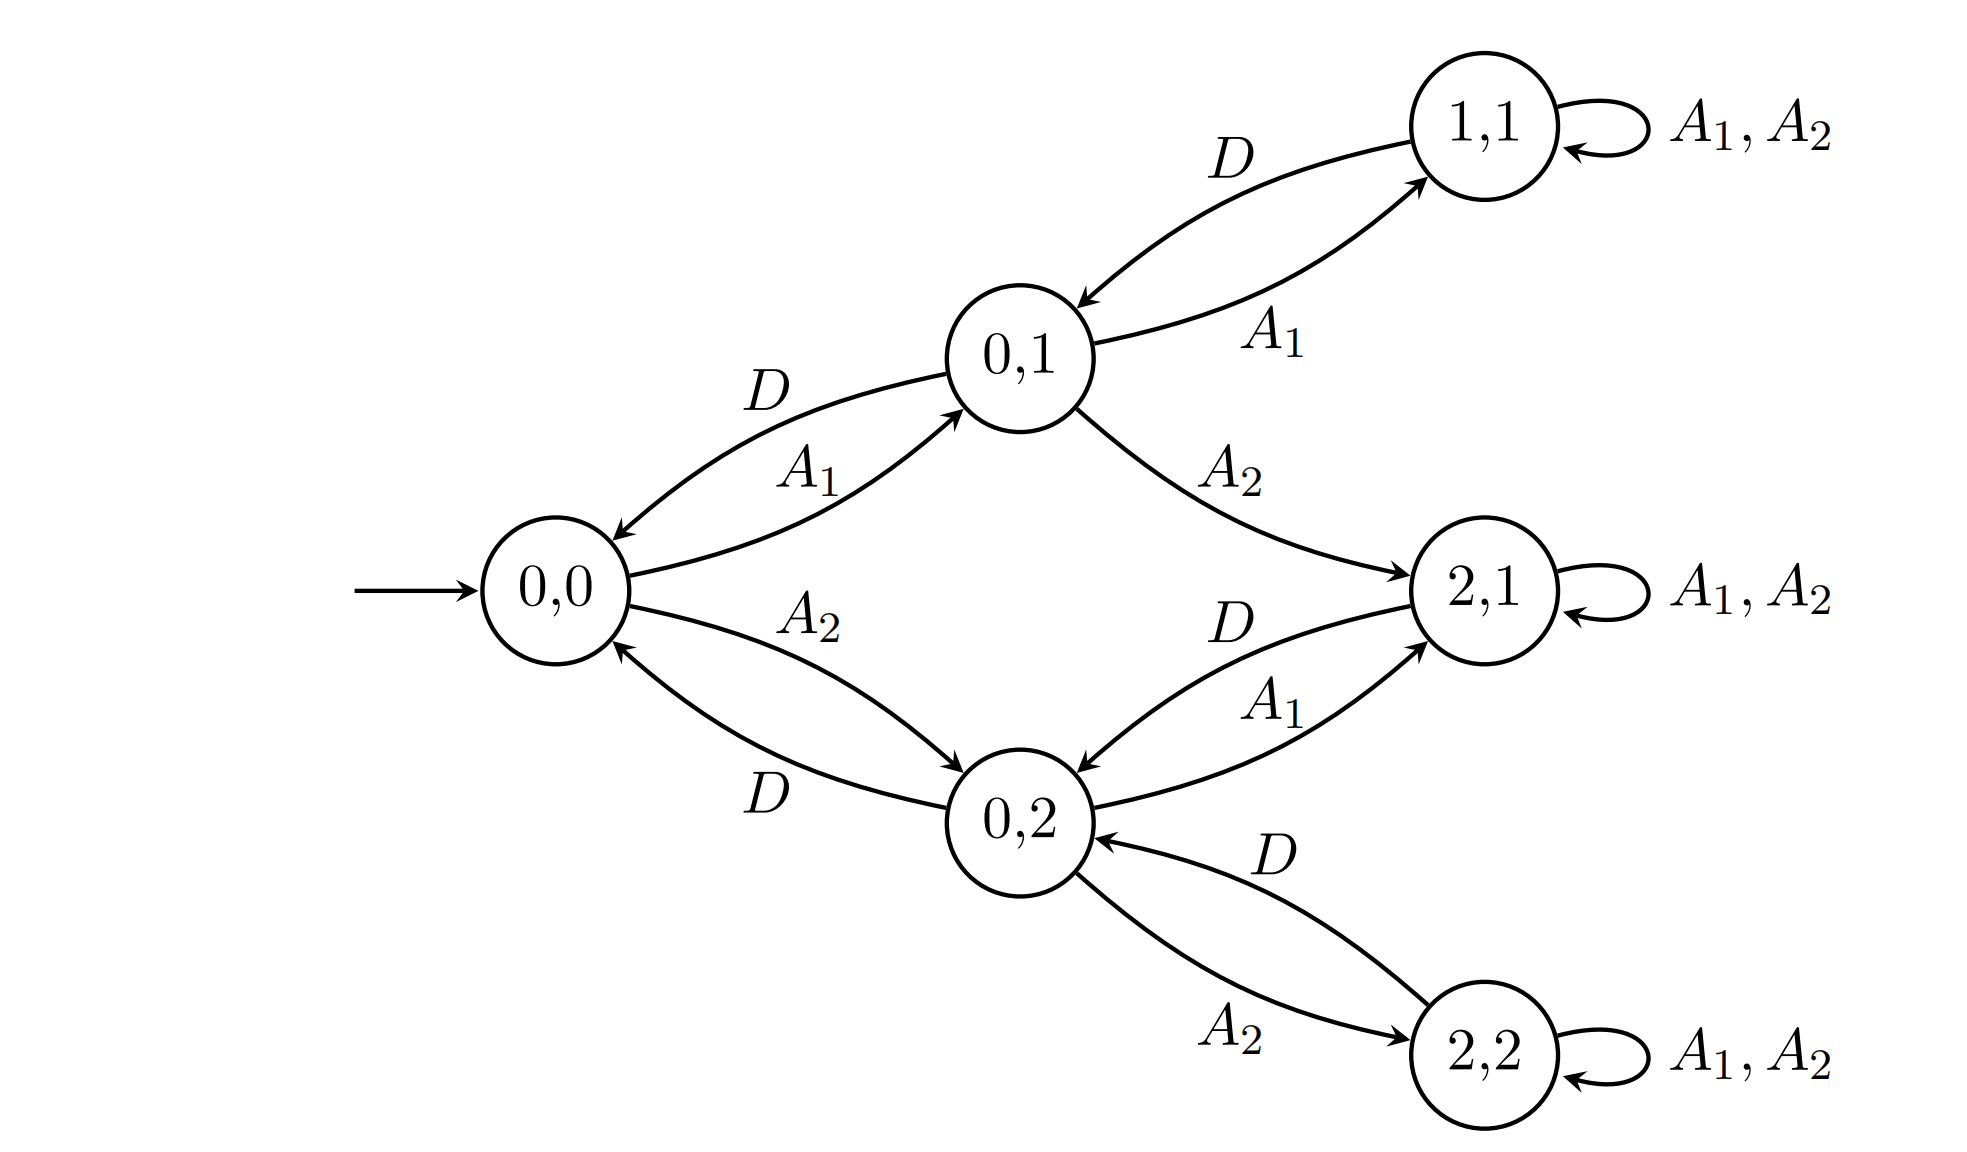
\includegraphics[width=0.6\textwidth]{assets/DES26.png}
  \caption{Toys}
  \label{fig:des26}
\end{figure}

\paragraph{Answer}:



%26
Figure \ref{fig:des26}

\section{A computer system operates with two parallel processors P1 and P2. The total capacity (queue and server included) of P1 is $K_1 = 1$, and that of P2 is $K_2 = 2$. The system receives two types of jobs, labeled $J_1$ and $J_2$. Jobs of type $J_1$ must be processed at P1, and jobs of type $J_2$ must be processed at P2. When a job is processed, it leaves the system. If a job finds a full queue upon arrival, then the job is simply rejected. Build an automaton model of this system.}

\begin{tcolorbox}
  Four events are identified: 
  
  $a_i$: arrival of $J_i$ 

  $d_i$: departure of $J_i$.
  
  A state is of the form ($n_1$, $n_2$) where $n_i$ is the number of jobs in (queue and server) in processor $P_i$. 
  
  Note that the model has six states totally.
\end{tcolorbox}

\paragraph{Answer}: 

%27

$$
A=\left(Y, \Sigma, \eta, y_0, Y_m\right)
$$
$\Sigma=\{11,12,22,21\}, 11$ means J1 comes in, 12 means J1 comes out, 22 means J2 comes in, 22 means $\mathrm{J} 2$ comes out.
$$
\begin{aligned}
& Y=\{0,1,2,3,4,5\} \\
& Y_m=\{0\}
\end{aligned}
$$



\begin{figure}[h]
  \centering
  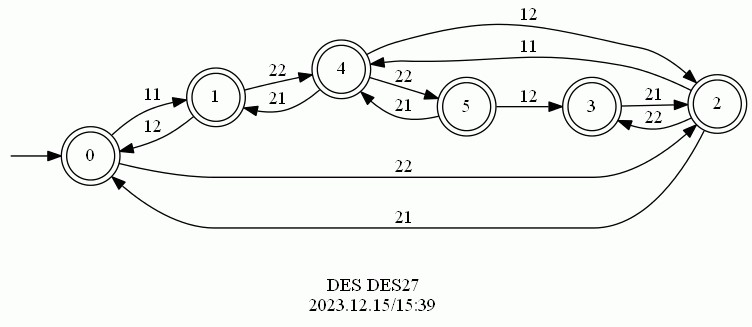
\includegraphics[width=\textwidth]{assets/DES27.jpg}
  \caption{Homework 27}
  \label{fig:des27}
\end{figure}

Figure \ref{fig:des27}

% States:

% \begin{itemize}
%   \item State (0, 0): Initial state. No jobs are in the system.
%   \item State (1, 0): A job of type $J_1$ is in the queue for P1.
%   \item State (2, 0): Two jobs of type J1 are in the queue for P1 (queue full, no room for $J_2$).
%   \item State (0, 1): A job of type $J_2$ is in the queue for P2.
%   \item State (0, 2): Two jobs of type $J_2$ are in the queue for P2 (queue full, no room for $J_1$).
%   \item State (1, 1): A job of type $J_1$ is in the queue for P1, and a job of type $J_2$ is in the queue for P2 (both queues occupied).
% \end{itemize}

% Transitions:

% \begin{enumerate}
%   \item From State (0, 0):
%   \begin{itemize}
%     \item On arrival of a job of type $J_1$, transition to State (1, 0).
%     \item On arrival of a job of type $J_2$, transition to State (0, 1).
%   \end{itemize}
%   \item From State (1, 0):
%   \begin{itemize}
%     \item On arrival of another job of type $J_1$, transition to State (2, 0) (queue for P1 is full).
%     \item On arrival of a job of type $J_2$, transition to State (1, 1) ($J_2$ joins P2's queue).
%     \item On departure of the $J_1$ job from P1, transition back to State (0, 0).
%   \end{itemize}
%   \item From State (2, 0):
%   \begin{itemize}
%     \item On arrival of a job of type $J_1$, stay in State (2, 0) (queue is full, job rejected).
%     \item On arrival of a job of type $J_2$, stay in State (2, 0) (queue is full, job rejected).
%     \item On departure of the $J_1$ job from P1, transition to State (0, 0) (queue for P1 is free).
%   \end{itemize}
%   \item From State (0, 1):
%   \begin{itemize}
%     \item On arrival of a job of type $J_1$, transition to State (1, 1) ($J_1$ joins P1's queue).
%     \item On arrival of another job of type $J_2$, transition to State (0, 2) (queue for P2 is full).
%     \item On departure of the $J_2$ job from P2, transition back to State (0, 0).
%   \end{itemize}
%   \item From State (0, 2):
%   \begin{itemize}
%     \item On arrival of a job of type $J_1$, stay in State (0, 2) (queue is full, job rejected).
%     \item On arrival of a job of type $J_2$, stay in State (0, 2) (queue is full, job rejected).
%     \item On departure of the $J_2$ job from P2, transition to State (0, 1) (queue for P2 is free).
%   \end{itemize}
%   \item From State (1, 1):
%   \begin{itemize}
%     \item On arrival of another job of type $J_1$, stay in State (1, 1) (both queues are full, job rejected).
%     \item On arrival of another job of type $J_2$, stay in State (1, 1) (both queues are full, job rejected).
%     \item On departure of the $J_1$ job from P1, transition to State (0, 1) (queue for P1 is free).
%     \item On departure of the $J_2$ job from P2, transition to State (1, 0) (queue for P2 is free).
%   \end{itemize}
  
% \end{enumerate}


\section{A workcell consists of two machines M1 and M2 and an automated guided vehicle AGV, along with two auxiliary devices: input buffer and output buffer whose capacity is assumed to be large enough.}

\paragraph{Answer}:

%28
\begin{figure}[h]
  \centering
  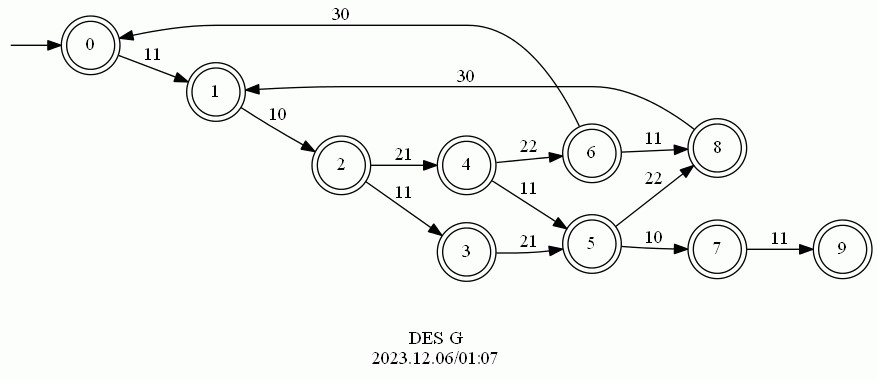
\includegraphics[width=\linewidth]{assets/findg.jpg}
  \caption{G}
  \label{fig:findg}
\end{figure}


\begin{enumerate}
  \item Find G 
  
  As shown in Figure \ref{fig:findg}.
  \item Check G is blocking or nonblocking (that can be done by using TCT)
  
  To check if G is blocking or nonblocking, we can use the TCT (Transition Closure Table) method. The TCT method involves iteratively computing the reachable states from the initial state and checking if there are any deadlock states (states from which no further transitions are possible).
  \item If G is not non-blocking, analyse the blocking states and the event sequences leading to the blocking states from the initial state
  
  If G is found to be blocking, we can analyze the blocking states and the event sequences leading to them from the initial state. Blocking states are states from which no further progress can be made, i.e., no transitions are enabled.
  \item Propose a supervisory control strategy such that the controlled system is non-blocking (one could use TCT to verify the proposed non-blocking strategy).
  
  To propose a supervisory control strategy that ensures non-blocking behavior, we can use the TCT method to verify the proposed strategy. The goal is to design a supervisor that allows the system to reach only non-blocking states and avoids deadlock or blocking situations.
\end{enumerate}

\section{Propose the Petri net model for the system in Question 28.}

\paragraph{Answer}:

%29

\begin{figure}
  \centering
  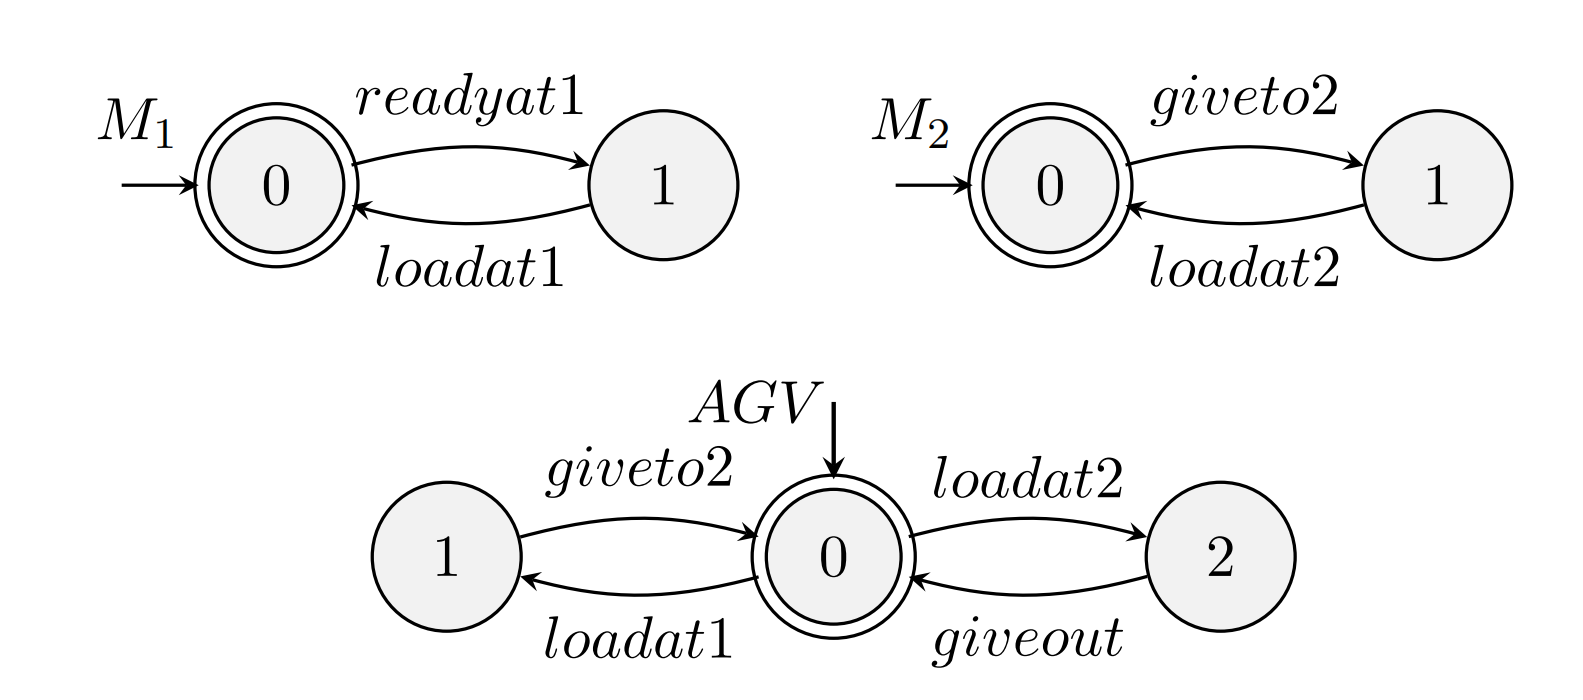
\includegraphics[width=0.5\linewidth]{assets/DES29.png}
  \caption{Petri net model}
  \label{fig:des29}
\end{figure}

Figure \ref{fig:des29}.


\section{Given $L, L_1, L_2, L_3 \subseteq  \Sigma^*$, show}

\begin{gather*}
  L \subseteq \overline{L}, \\
  \overline{ L_1 \cap L_2 } \subseteq \overline{L_1} \cap \overline{L_2}, \\
  L_1(L_2 \cup L_3) = L_1L_2 \cup L_1L_3, and. \\
  L_1(L_2 \cap L_3) = L_1L_2 \cap L_1L_3.
\end{gather*}

\paragraph{Answer}:

%30

\begin{itemize}
  \item $L \subseteq \overline{L}$
  
  To show that a language $L$ is a subset of its complement, you want to prove that for every string $x$ in $L$, it is also in $\overline{L}$, which means that $L \subseteq \overline{L}$.

  Here's the formal proof:

  Let $x$ be an arbitrary string in $L$. This means that $x$ is an element of $L$. Since $x$ is in $L$, it is also not in $\overline{L}$, by definition. Therefore, $x$ is in $L$ and not in $\overline{L}$.

  Because $x$ was an arbitrary string chosen from $L$, this proof holds for all strings in $L$. Therefore, we can conclude that for every string $x$ in $L, x$ is also in $\overline{L}$, which means $L \subseteq \overline{L}$.

  In other words, the entire language $L$ is a subset of its own complement $\overline{L}$.

  \item $\overline{ L_1 \cap L_2 } \subseteq \overline{L_1} \cap \overline{L_2}$
  
  To show that $\overline{L_1 \cap L_2} \subseteq \overline{L_1} \cap \overline{L_2}$, we need to prove that if a string is in the complement of the intersection of two languages $L_1$ and $L_2$, then it is also in the intersection of the complements of these languages.

  Let's use set notation to represent this:
  
  $\overline{L_1 \cap L_2}$ represents the complement of the intersection of $L_1$ and $L_2$.
  
  $\overline{L_1} \cap \overline{L_2}$ represents the intersection of the complements of $L_1$ and $L_2$.
  
  We want to prove that for any string $x$:
  
  If $x \in \overline{L_1 \cap L_2}$, then $x \in \overline{L_1} \cap \overline{L_2}$.
  
  Here's the proof:
  
  Suppose $x \in \overline{L_1 \cap L_2}$. This means that $x$ is not in the intersection of $L_1$ and $L_2$. In other words, $x \notin (L_1 \cap L_2)$.
  
  Now, we can use De Morgan's Law, which states that the complement of an intersection is equal to the union of complements:
  
  $\overline{L_1 \cap L_2} = \overline{L_1} \cup \overline{L_2}$
  
  So, we have $x \in (\overline{L_1} \cup \overline{L_2})$. This means that $x$ is in either the complement of $L_1$ or the complement of $L_2$, or both.
  
  Therefore, $x \in \overline{L_1}$ and $x \in \overline{L_2}$.
  
  This is precisely what is represented by $x \in \overline{L_1} \cap \overline{L_2}$, which is the intersection of the complements of $L_1$ and $L_2$.
  
  So, we have shown that if $x \in \overline{L_1 \cap L_2}$, then $x \in \overline{L_1} \cap \overline{L_2}$, which proves the inclusion $\overline{L_1 \cap L_2} \subseteq \overline{L_1} \cap \overline{L_2}$.

  \item $L_1(L_2 \cup L_3) = L_1L_2 \cup L_1L_3$
  
  To prove that $L_1(L_2 \cup L_3) = L_1L_2 \cup L_1L_3$, we need to show that every string in the left-hand side (LHS) language is also in the right-hand side (RHS) language, and vice versa.

  Let's break this proof into two parts:
  
  Part 1: Proving $L_1(L_2 \cup L_3) \subseteq L_1L_2 \cup L_1L_3$:
  
  Let $x$ be a string in $L_1(L_2 \cup L_3)$. This means that $x$ is of the form $x = yz$, where $y \in L_1$ and $z \in (L_2 \cup L_3)$. Since $z \in (L_2 \cup L_3)$, it means that $z$ can be either in $L_2$ or $L_3$.
  
  \begin{enumerate}
    \item If $z \in L_2$, then $yz$ is in $L_1L_2$, and therefore, $x$ is in $L_1L_2 \cup L_1L_3$.
    
    \item If $z \in L_3$, then $yz$ is in $L_1L_3$, and therefore, $x$ is in $L_1L_2 \cup L_1L_3$.
  \end{enumerate}
  
  In both cases, $x$ is in $L_1L_2 \cup L_1L_3$. Therefore, we have shown that $L_1(L_2 \cup L_3) \subseteq L_1L_2 \cup L_1L_3$.
  
  Part 2: Proving $L_1(L_2 \cup L_3) \supseteq L_1L_2 \cup L_1L_3$:
  
  Let $x$ be a string in $L_1L_2 \cup L_1L_3$. This means that $x$ is either in $L_1L_2$ or $L_1L_3$.
  
  \begin{enumerate}
    \item If $x$ is in $L_1L_2$, it means $x = yz$, where $y \in L_1$ and $z \in L_2$. Since $z \in L_2$, we can say that $z$ is in $(L_2 \cup L_3)$, and therefore, $x$ is in $L_1(L_2 \cup L_3)$.
    \item If $x$ is in $L_1L_3$, it means $x = yz$, where $y \in L_1$ and $z \in L_3$. Similar to the first case, since $z \in L_3$, we can say that $z$ is in $(L_2 \cup L_3)$, and therefore, $x$ is in $L_1(L_2 \cup L_3)$.
  \end{enumerate}
  
  In both cases, $x$ is in $L_1(L_2 \cup L_3)$. Therefore, we have shown that $L_1(L_2 \cup L_3) \supseteq L_1L_2 \cup L_1L_3$.
  
  Combining both parts, we have proven that $L_1(L_2 \cup L_3) = L_1L_2 \cup L_1L_3$.

  \item $L_1(L_2 \cap L_3) = L_1L_2 \cap L_1L_3$
  
  To prove that $L_1(L_2 \cap L_3) = L_1L_2 \cap L_1L_3$, we need to show that every string in the left-hand side (LHS) language is also in the right-hand side (RHS) language, and vice versa.

  Let's break this proof into two parts:

  Part 1: Proving $L_1(L_2 \cap L_3) \subseteq L_1L_2 \cap L_1L_3$:

  Let $x$ be a string in $L_1(L_2 \cap L_3)$. This means that $x$ is of the form $x = yz$, where $y \in L_1$ and $z \in (L_2 \cap L_3)$. Since $z \in (L_2 \cap L_3)$, it means that $z$ is in both $L_2$ and $L_3$.

  \begin{enumerate}
    \item Since $y \in L_1$ and $z \in L_2$, $yz$ is in $L_1L_2$, and therefore, $x$ is in $L_1L_2 \cap L_1L_3$.
    \item Since $y \in L_1$ and $z \in L_3$, $yz$ is in $L_1L_3$, and therefore, $x$ is in $L_1L_2 \cap L_1L_3$.
  \end{enumerate}
  

  In both cases, $x$ is in $L_1L_2 \cap L_1L_3$. Therefore, we have shown that $L_1(L_2 \cap L_3) \subseteq L_1L_2 \cap L_1L_3$.

  Part 2: Proving $L_1(L_2 \cap L_3) \supseteq L_1L_2 \cap L_1L_3$:

  Let $x$ be a string in $L_1L_2 \cap L_1L_3$. This means that $x$ is in both $L_1L_2$ and $L_1L_3$.

  \begin{enumerate}
    \item If $x$ is in $L_1L_2$, it means $x = yz$, where $y \in L_1$ and $z \in L_2$. Since $z \in L_2$, it follows that $z$ is in $L_2 \cap L_3$, and therefore, $x$ is in $L_1(L_2 \cap L_3)$.
    \item If $x$ is in $L_1L_3$, it means $x = yz$, where $y \in L_1$ and $z \in L_3$. Similar to the first case, $z$ is in $L_2 \cap L_3$, and therefore, $x$ is in $L_1(L_2 \cap L_3)$.
  \end{enumerate}
  
  In both cases, $x$ is in $L_1(L_2 \cap L_3)$. Therefore, we have shown that $L_1(L_2 \cap L_3) \supseteq L_1L_2 \cap L_1L_3$.

  Combining both parts, we have proven that $L_1(L_2 \cap L_3) = L_1L_2 \cap L_1L_3$.

\end{itemize}




\section{Let G be a generator with the alphabet $\Sigma$ and $K \subseteq \Sigma^*$ be a language. Show $\overline{K} \subseteq L(G)$ if $K \subseteq L(G)$: [hint: L(G) is prefix-closed].}

\paragraph{Proof}:
%31

To show that $\overline{K} \subseteq L(G)$ given that $K \subseteq L(G)$ and $L(G)$ is prefix-closed, we can use the fact that $L(G)$ being prefix-closed implies that it contains all the prefixes of its language. 

Since $K \subseteq L(G)$, every prefix of a word in $K$ is also a prefix of a word in $L(G)$. But $L(G)$ is prefix-closed, which means that it contains all its prefixes. Therefore, every prefix of a word in $K$ is also in $L(G)$. 

Now, let's consider $\overline{K}$, which represents the complement of $K$. This means that $\overline{K}$ contains all the words that are not in $K$. Since $L(G)$ contains every prefix of a word in $K$, it follows that $L(G)$ also contains every prefix of a word in $\overline{K}$. 

Therefore, we can conclude that $\overline{K} \subseteq L(G)$, as every prefix of a word in $\overline{K}$ is also in $L(G)$. This result holds under the assumption that $K \subseteq L(G)$ and $L(G)$ is prefix-closed.



\section{Given a generator G with $\Sigma = \{a, b, c\}$ as shown below, assume that b is not observable. Find P (G).}

\paragraph{Answer}:
%32

\begin{figure}[h]
  \centering
  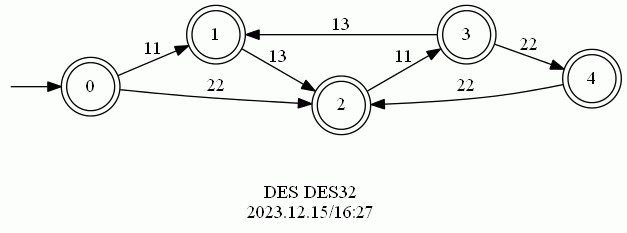
\includegraphics{assets/DES32.jpg}
  \caption{Homework 32}
  \label{fig:des32}
\end{figure}

\begin{table}
  \centering
  \begin{tabular}{|c|c|}
    $q$ & 11\\
    $b$ & 22\\
    $c$ & 13\\
  \end{tabular}
  \caption{Homework32}
  \label{tab:des32}
\end{table}

Figure \ref{fig:des32}, events in table \ref{tab:des32}

\section{Show the properties of projection.}

\begin{enumerate}
  \item If $A \subseteq B$, $P A \subseteq P B$ and $P^{-1}A \subseteq P^{-1}B$.
  \item $P [P^{-1}(L)] = L$; $L \subseteq P^{-1}[P (L)]$.
  \item $P (A \cup B) = P A \cup P B$.
  \item $P^{-1} (A \cup B) = P^{-1} (A) \cup P^{-1} (B)$; $P^{-1} (A \cap B) = P^{-1} (A) \cap P^{-1} (B)$.
  \item $P (AB) = P (A)P (B); P^{-1} (AB) = P^{-1} (A)P^{-1}(B)$.
\end{enumerate}

\paragraph{Answer}:
%33

Chapter 4. page:89

\begin{enumerate}
  \item If $A \subseteq B$, then $PA \subseteq PB$ and $P^{-1}A \subseteq P^{-1}B$.
  
  Proof:

  Let $s \in PA$. There necessarily exist $t \in \Sigma^*$ such that $t \in A$ and $Pt = s$. By $A \subseteq B$, $t \in B$. We have $Pt = s \in PB$
  
  Let $s \in P^{-1}A$. Then there exist $t \in A$ such that $Ps = t$. By $A \subseteq B$, $Ps \in B$ and $s\in P^{-1}B$

  In the proof above, from $Ps \in B$, we cannot directly infer $P^{-1}[Ps] \subseteq P^{-1}B$ and cannot derive $s \in P^{-1}B$ by $s \in P^{-1}[Ps]$.

  Portray $Ps \in B$ naturally means $s \in P^{-1}B$

  \item $P[P^{-1}(L)] = L$; $L \subseteq P^{-1}[P(L)]$.
  

  \begin{enumerate}
    \item $P[P^{-1}(L)] = L$
    
    Proof:

    To show $P[P^{-1}(L)] \subseteq L$, we need to prove $P[P^{-1}(L)] \subseteq L$ and $L \subseteq P[P^{-1}(L)]$.
  
    \begin{itemize}
      \item let $s \in P[P^{-1}(L)]$, there necessarily exists $t \in \Sigma^*$ such that $t \in P^{-1}(L)$ and $Pt = s$. By $t \in P[P^{-1}(L)]$, $Pt \in L$(Note that $P^{-1}(L) = \{s\prime \in \Sigma^* | (\exists s \in L)Ps\prime = s\}$). We have $Pt = s \in L$ and thus $P[P^{-1}(L)] \subseteq L$
      \item To show $L \subseteq P[P^{-1}(L)]$, let $s \in L$. $P^{-1}\{s\} \subseteq P^{-1}(L)$. $P[P^{-1}\{s\}] \subseteq P[P^{-1}(L)]]$ (by Property 1). By $s \in P[P^{-1}\{s\}]$, $s \in P[P^{-1}(L)]$ then $L \subseteq P[P^{-1}(L)]$ holds.
    \end{itemize}
      
    \item $L \subseteq P^{-1}[P(L)]$
    
    Proof:

    let $s \in L$. 

    $\{s\} \subseteq L \Rightarrow P\{s\} \subseteq PL \Rightarrow P^{-1}[P\{s\}] \subseteq P^{-1}[P(L)]$.

    By $s \in P^{-1}[P\{s\}]$, we have $s \in P^{-1}[P(L)]$. 

    We conclude $L \subseteq P^{-1}[P(L)]$.

  \end{enumerate}
  
  \item $P(A \cup B) = P(A) \cup P(B)$.
  
  Proof:
  
  ($\subseteq$) Let $s \in P(A \cup B)$. There necessarily exists $t \in \Sigma^*$ such that $t \in A \cup B$ and $Pt = s$. We have three cases:

  \begin{itemize}
    \item[(i)] $t \in A$ and $t \notin B$. Then $Pt \in PA$, i.e., $s \in PA$. Thus, $s \in PA \cup PB$
    \item[(ii)] $t \in B$ and $t \notin A$. Then $Pt \in PB$, i.e., $s \in PB$. Thus, $s \in PA \cup PB$
    \item[(iii)] $t \in A$ and $t \in B$. Then $Pt \in PA$ and $Pt \in PB$. Thus, $s \in PA \cup PB$
  \end{itemize}

  Finally, we have $P(A \cup B) \subseteq P(A) \cup P(B)$.

  ($\supseteq$) Let $s \in P(A) \cup P(B)$. Then two cases are considered.

  \begin{itemize}
    \item[(i)] $s \in P(A)$ and $s \notin P(B)$(or $[s \in P(B) \& s \notin P(A)]$). There exists $t \in \Sigma^*$ such that $t \in A$ and $Pt = s$. Then, we have $t \in A \cup B$ and $Pt = s \in P(A \cup B) $.
    \item[(ii)] $s \in P(A)$ and $s \in P(B)$. There exists $t_1 \in \Sigma^*$ and $t_2 \in \Sigma^*$ such that $t_1 \in A$, $t_2 \in B$ and $Pt_1 = Pt_2 = s$. $t_1 \in A \cup B$, $Pt_1 = s \in P(A \cup B)$. Thus, $PA \cup PB \subseteq P(A \cup B)$.
  \end{itemize}

  
  \item $P^{-1}(A \cup B) = P^{-1}(A) \cup P^{-1}(B)$; $P^{-1}(A \cap B) = P^{-1}(A) \cap P^{-1}(B)$.
  
  \begin{enumerate}
    \item $P^{-1}(A \cup B) = P^{-1}(A) \cup P^{-1}(B)$.
    
    Proof:
    
    ($\subseteq$) $P^{-1}(A \cup B) \subseteq P^{-1}(A) \cup P^{-1}(B)$.

    Let $s \in P^{-1}(A \cup B)$. $(\exists t \in \Sigma^*) t \in A \cup B$ such that $Ps = t$.
    
    \begin{itemize}
      \item[(i)] $Ps \in A$, $Ps \notin B$
      
      $P^{-1}(Ps) \subseteq P^{-1}(A)$. $s \in P^{-1}(Ps)$, $s \in P^{-1}(A)$

      $s \in P^{-1}(A) \Rightarrow s \in P^{-1}(A) \cup P^{-1}(B)$.

      \item[(ii)] $Ps \notin A$, $Ps \in B$
      
      $P^{-1}(\{Ps\}) \subseteq P^{-1}(B)$.
      
      $s \in P^{-1}(Ps)$, $s \in P^{-1}(B) \Rightarrow s \in P^{-1}(B) \cup P^{-1}(A)$

      \item[(iii)] $Ps \in A$, $Ps \in B$
      
      $P^{-1}(\{Ps\}) \subseteq P^{-1}(A)$ and $P^{-1}(Ps) \subseteq P^{-1}(B)$

      By $s \in P^{-1}(\{Ps\})$, then

      $s \in P^{-1}(A)$, $s \in P^{-1}(B)$, $s \in P^{-1}(A) \cup P^{-1}(B)$ 

    \end{itemize}

    ($\supseteq$) Show $P^{-1}(A) \cup P^{-1}(B) \supseteq P^{-1}(A \cup B)$.

    Let $s \in P^{-1}(A) \cup P^{-1}(B)$. Three cases:

    \begin{itemize}
      \item[(i)] $s \in P^{-1}(A)$, $s \notin P^{-1}(B)$
      
      $Ps \in A \Rightarrow Ps \in A \cup B$

      $P^{-1}(\{Ps\}) \subseteq P^{-1}(A \cup B)$

      By $s \in P^{-1}(\{Ps\})$, $s \in P^{-1}(A \cup B)$.

      \item[(ii)] $s \in P^{-1}(B)$, $s \notin P^{-1}(A)$ (similar to (i))
      
      \item[(iii)] $s \in P^{-1}(A)$ and $s \in P^{-1}(B)$
      
      $Ps \in A$, $Ps \in B \Rightarrow Ps \in A \cup B$

      $P^{-1}(\{Ps\}) \subseteq P^{-1}(A \cup B)$

      $s \in P^{-1}(\{Ps\}) \Rightarrow s \in P^{-1}(A \cup B)$


    \end{itemize}

    Finally, we have

    $P^{-1}(A \cup B) = P^{-1}(A) \cup P^{-1}(B)$


    
    \item $P^{-1}(A \cap B) = P^{-1}(A) \cap P^{-1}(B)$.
    
    Proof:
    
    ($\subseteq$) Let $s \in P^{-1}(A \cap B)$.

    $(\exists t \in \Sigma^*) t \in A \cap B$ and $Ps = t$

    $t \in A$ and $t \in B$

    Since $s \in P^{-1}(\{Ps\}) = P^{-1}\{t\}$, $s \in P^{-1}(A)$ and $s \in P^{-1}(B)$

    $s \in P^{-1}(A) \cap P^{-1}(B)$

    ($\supseteq$) Let $s \in P^{-1}(A) \cap P^{-1}(B)$, i.e., $s \in P^{-1}(A)$ and $s \in P^{-1}(B)$

    $Ps \in A$ and $Ps \in B$ $Ps \in (A \cap B)$

    $P^{-1}(\{Ps\}) \subseteq P^{-1}(A \cap B)$

    By $s \in P^{-1}(\{Ps\})$, $s \in P^{-1}(A \cap B)$

    $P^{-1}(A) \cap P^{-1}(B) \subseteq P^{-1}(A \cap B)$.



    
  \end{enumerate}  
  \item $P(AB) = P(A)P(B)$; $P^{-1}(AB) = P^{-1}(A)P^{-1}(B)$.

  \begin{enumerate}
    \item $P(AB) = P(A)P(B)$.
    
    Proof:
    
    ($\subseteq$) Let $s \in P(AB)$. $(\exists t \in \Sigma^*) t \in AB$ and $Ps = t$. Since

    $AB = \{s_1s_2 \mid s_1 \in A, s_2 \in B\}$,

    Let $t = t_1t_2$ with $t_1 \in A$ and $t_2 \in B$.

    $Pt = Pt_1 \cdot Pt_2 \in P(A)P(B)$

    $s \in P(A)P(B)$

    ($\supseteq$) Let $s \in P(A)P(B)$ with $s = s_1s_2$.

    $P(A)P(B) = \{s_1s_2 \mid s_1 \in P(A), s_2 \in P(B)\}$

    $s_1 \in P(A) \Rightarrow \exists t_1 \in A Pt_1 = t_1$

    $s_2 \in P(B) \Rightarrow \exists t_2 \in B Pt_2 = t_2$

    By $t_1t_2 \in AB$, $P(t_1t_2) = P(t_1)P(t_2) = s_1s_2 = s \in P(AB)$.


    
    \item $P^{-1}(AB) = P^{-1}(A)P^{-1}(B)$.
    
    Proof:
    
    ($\subseteq$) Let $s \in P^{-1}(AB)$. $Ps \in AB$

    $(\exists s_1s_2 \in \Sigma^*) Ps_1 \in A$, $Ps_2 \in B$, $s = s_1s_2$

    $p^{-1}(Ps_1) \subseteq P^{-1}(A)$, $p^{-1}(Ps_2) \subseteq P^{-1}(B)$

    Since $s_1 \in P^{-1}(Ps_1)$, $s_2 \in P^{-1}(Ps_2)$

    $s_1s_2 \in P^{-1}(A)P^{-1}(B)$

    ($\supseteq$) Let $s \in P^{-1}(A)P^{-1}(B)$

    $(\exists t_1t_2 \in \Sigma^*) t_1 \in A$, $t_2 \in B$ $Ps=t_1t_2$

    $t_1t_2 \in AB$, $P{-1}(t_1t_2) \subseteq P^{-1}(AB)$. $P^{-1}(Ps) \subseteq P^{-1}(AB)$.

    $s \in P^{-1}(Ps) \Rightarrow s \in P^{-1}(AB)$.



    
  \end{enumerate}
  
  Proof: (to be completed)
\end{enumerate}

\section{Given H, K, L, and $\Sigma = \Sigma_c \dot{\cup} \Sigma_u$ such that $H \subseteq K = K \subseteq L = L \subseteq \Sigma^*$, suppose that H is controllable with respect to K and $\Sigma_u$ and K is controllable with respect to L and $\Sigma_u$. Show that H is controllable with respect to L and $\Sigma_u$ (check whether $L = \overline{L}$ is a necessity for the controllability of H with respect to L and $\Sigma_u$).}

\paragraph{Proof}:
%34
We know the defination of controllable Let $K \subseteq \Sigma^*(K=\emptyset)$. K is controllable with respect to $\mathrm{H}$ if
$$
\begin{array}{r}
\bar{K} \Sigma_u \cap L(H) \subseteq \bar{K} \\
\bar{K} \Sigma_u=\left\{s \in \Sigma^* \mid s=s^{\prime} \sigma, \sigma \in \Sigma_u, s^{\prime} \in K\right\}
\end{array}
$$
Equivalently, $\left(\forall s \in \Sigma^*\right)(\forall \sigma \in \Sigma) s \in K$ and $\sigma \in \Sigma_u$ and $s \sigma \in L(H) \Rightarrow s \sigma \in$
$K$
For exmple $L_1=\{\alpha \lambda \mu\}$ and $\overline{L_1}=\{\varepsilon, \alpha, \alpha \lambda, \alpha \lambda \mu\}$. L is uncontrollable since $s=\alpha \in \bar{K}, \beta \in \Sigma_u, \alpha \beta \in L(H)[\alpha \beta \notin \bar{K}]$. For $s=\alpha, \sigma=\beta$ or $\lambda$

Test $\lambda: \lambda \alpha \in K\left(\lambda \in \Sigma_u\right)$ controllable


Test $\beta: \alpha \beta \notin L_1$ uncontrollable. Thus $L_1$ is uncontrollable.

\section{Let MACH as depicted below be a generator with $\Sigma = \{\alpha , \beta , \lambda , \mu \}$, where $\alpha$ and $\mu$ are controllable. Suppose that the SPEC is $K = \{\alpha\beta\alpha\beta\}$, i.e., MACH is shut down after two successful production cycles. By intuition, check if there exists a supervisor that can supervise MACH to implement this SPEC. If existing, portray it; otherwise, explain the reason of non-existence. Consider the case that $K = \{\alpha\beta\}$.}

\paragraph{Answer}:
%35

As Figure \ref{fig:des35} shows.

\begin{figure}[h]
  \centering
  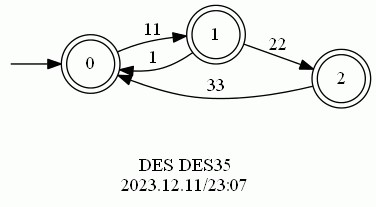
\includegraphics{assets/DES35.jpg}
  \caption{Homework 35}
  \label{fig:des35}
\end{figure}

\section{Review the notion of equivalence relation and propose 2-3 examples of equivalence relations in our daily life.}

\paragraph{Answer}:
%36
\begin{enumerate}
  \item Friendship: Consider a group of friends. We can define an equivalence relation on this group based on friendship. Two individuals are related if they are friends with each other. This relation is reflexive (everyone is a friend of themselves), symmetric (if person A is a friend of person B, then person B is a friend of person A), and transitive (if person A is a friend of person B, and person B is a friend of person C, then person A is a friend of person C).
  \item Equality: In mathematics, the relation of equality is an equivalence relation. Two numbers are related if they are equal to each other. This relation is reflexive (every number is equal to itself), symmetric (if a = b, then b = a), and transitive (if a = b and b = c, then a = c).
  \item Language: In linguistics, we can define an equivalence relation based on language dialects. Two individuals are related if they speak the same dialect. This relation is reflexive (everyone speaks the dialect they are associated with), symmetric (if person A speaks the same dialect as person B, then person B speaks the same dialect as person A), and transitive (if person A speaks the same dialect as person B, and person B speaks the same dialect as person C, then person A speaks the same dialect as person C).
\end{enumerate}


\section{Given a plant G with some control specification}
Given a plant $G$ with some control specification, the set of control patterns is $\Gamma=\left\{\gamma \mid \Sigma_u \subseteq \gamma\right\}$, i.e., a control pattern $\gamma$ is usually a super-set of $\Sigma_u$. Suppose that $V$ is a supervisory control function that implements the control specification. Given $s \in L(G), V(s) \in \Gamma$ defines the set of events that are feasible or active after $s$ is generated by $G$. It implies that the events in $\Sigma-V(s)$ should be disabled upon the occurrence of $s$.

Let $f(s)=\Sigma-V(s)$. The generated language $L(f / G)$ and the marked language $L_m(f / G)$ of the controlled system under the supervision of $f$ are respectively defined as
\begin{enumerate}
  \item $\varepsilon \in L(f / G) ;\left(\forall s \in \Sigma^*\right)(\forall \sigma \in \Sigma)[s \in L(f / G)] \&[s \sigma \in L(G)] \&[\sigma \notin f(s)] \Rightarrow s \sigma \in L(f / G)$.
  \item $L_m(f / G)=L(f / G) \cap L_m(G)$
\end{enumerate}

\paragraph{Answer}:
%37
\begin{enumerate}
  \item Obviously, $L(f/ G) \subseteq \overline{L(f/ G)}$
  \item To show $\overline{L(f/ G)} \subseteq L(f/ G)$, let $s \in \overline{L(f/ G)}$.
\end{enumerate}
Then, $\left(\exists t \in \Sigma^*\right)$ st $\in L(f/ G)$.
By induction, let $t=\varepsilon$ or $t=\sigma \in \Sigma$.
Then $s \in L(f/ G)$ (by definition of $L(f/ G)$ ).
(continued) Suppose that $s \in L(f/ G), t=\sigma_1 \sigma_2 \cdots \sigma_k$, and $s t \in L(f/ G)$, where $\sigma_i \in \Sigma, i \in \mathbb{N}_k$.

We will show $s \in L(f/ G)$ if $t=\sigma_1 \sigma_2 \cdots \sigma_k \sigma_k+1$ and $s t \in L(f/ G)$. Then,
$$
\sigma_{k+1} \in V\left(s \sigma_1 \sigma_2 \cdots \sigma_k\right)
$$
and
$$
s \sigma_1 \sigma_2 \cdots \sigma_k \sigma_{k+1} \in L(G)
$$
By $s \sigma_1 \sigma_2 \cdots \sigma_k \in L(f/ G)$ (by assumption) and $s \sigma_1 \sigma_2 \cdots \sigma_k \in L(G)[$ since $\mathrm{L}(\mathrm{G})$ is closed],
$$
\sigma_k \in V\left(s \sigma_1 \sigma_2 \cdots \sigma_{k-1}\right)
$$
Thus, $s \sigma_1 \sigma_2 \cdots \sigma_{k-1} \in L(f/ G)$. By induction, we reach $s \sigma_1 \in L(f/ G)$, implying that $s \in L(f/ G), \sigma_1 \in V(s), s \sigma_1 \in L(G)$. Thus it holds $s \in L(f/ G)$.



\section{Given $K \subseteq \Sigma^*$, prove that there exists a $\Sigma_u$-enabling, non-marking, and non-blocking supervisor such that $L(G||S) = K$ if and only if $\emptyset \neq  K = \overline{K} = \overline{L_m(G) \cap K} $ and $K$ is controllable.}

%38

\section{Let $G$ be a plant and $K_1,K_2 \subseteq \Sigma^*$ be the desired and generated language under supervision, respectively. Prove that there exists a $\Sigma_u$-enabling, non-marking, and non-blocking supervisor $S$ such that $L_m(G||S) =K_1$ and $L(G||S) = K_2$ if and only if.}
\begin{enumerate}
  \item $\overline{K_1}=K_2 \neq \emptyset$
  \item $K_1$ is relative closed with respect to $L_m(G)$, and
  \item $K_2$ is controllable.
\end{enumerate}

\paragraph{Answer}:
%39

$K_1$ is $L_m(G)$-closed, then $K_1=K_1 \cap L_m(G) K_2$ is $L_m(G)$-closed, then

\begin{equation*}
  \begin{aligned}
  K_2&=\overline{K_2} \cap L_m(G) \\
   K_1 \cap K_2&=\overline{K_1} \cap L_m(G) \cap \overline{K_2} \cap L_m(G)=\overline{K_1} \cap \overline{K_2} \cap L_m(G)
  \end{aligned}
\end{equation*}

$\text { So, } K_1 \cap K_2 \text { is } L_m(G) \text {-closed and controllable. }$

\section{Let $G$ be a trim automaton with $L_m(G)=\left(\alpha \gamma^* \beta\right)^*$. Let $K=(\alpha \beta)^*$ and $\Sigma_{u c}=\{\alpha, \beta\}$. }

\begin{enumerate}
  \item[(a)] Find a supervisor $S$ such that $L_m(S / G)=K$ and check whether $S$ is nonblocking;
  \item[(b)] If we cannot find a nonblocking supervisor $S$ such that $L_m(S / G)=K$, explain your reasoning;
  \item[(c)] Portray $L_m(G)$ and $K$ and use TCT to verify the reached conclusion.
\end{enumerate}

\paragraph{Answer}:
%40

\begin{figure}[h!]
  \centering
  \begin{subfigure}[b]{0.2\linewidth}
    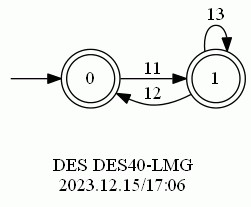
\includegraphics[width=\linewidth]{assets/DES40-LMG.jpg}
     \caption{$L_m(G)$.}
  \end{subfigure}
  \begin{subfigure}[b]{0.2\linewidth}
    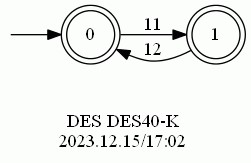
\includegraphics[width=\linewidth]{assets/DES40-K.jpg}
    \caption{$K$.}
  \end{subfigure}
  \caption{Homework40}
  \label{fig:des40}
\end{figure}

\begin{table}
  \centering
  \begin{tabular}{|c|c|}
    $\alpha$ & 11\\
    $\beta$ & 12\\
    $\gamma$ & 13\\
  \end{tabular}
  \caption{Homework40}
  \label{tab:des40}
\end{table}

Figure \ref{fig:des40}, Events in Table \ref{tab:des40}

\section{Let $L(G)=\overline{\left\{u_1 \alpha \gamma, u_1 \alpha \beta, u_2 \alpha \gamma\right\}}$, where $\Sigma=\Sigma_c$ and $E_{u o}=\left\{u_1, u_2\right\}$ (an event is controllable even if it is unobservable). (a) Let $K_1=\overline{\left\{u_1 \alpha \gamma, u_1 \alpha \beta\right\}}$. Find, if possible, a (partially observable) supervisor $S_P$ such that $L\left(S_P / G\right)=K_1 ;$ (b) Let $K_2=\overline{\left\{u_1 \alpha \gamma, u_1 \alpha \beta, u_2 \alpha\right\}}$. Find, if possible, a (partially observable) supervisor $S_P$ such that $L\left(S_P / G\right)=K_2$. Use TCT to verify the obtained results.}

\paragraph{Answer}:
%41
wait

\section{Consider $\sigma=\left\{\alpha_1, \beta_1, \gamma_1, \alpha_2, \beta_2, \gamma_2\right\}$ and a string $s=\alpha_1 \gamma_1 \alpha_2 \gamma_1$. Build an automaton $G$ such that $L(G)=$ $\Sigma^* \backslash \Sigma^*\{s\} \Sigma^*$. Analyze the reason why $G$ satisfies the requirement.}

\paragraph{Answer}:
%42
wait

\begin{table}
  \centering
  \begin{tabular}{|c|c|}
    $\alpha_1$ & 11\\
    $\alpha_2$ & 12\\
    \hline
    $\beta_1$ & 21\\
    $\beta_2$ & 22\\
    \hline
    $\gamma_1$ & 31\\
    $\gamma_2$ & 32\\
  \end{tabular}
  \caption{Homework42}
  \label{tab:des42}
\end{table}

\begin{figure}
  \centering
  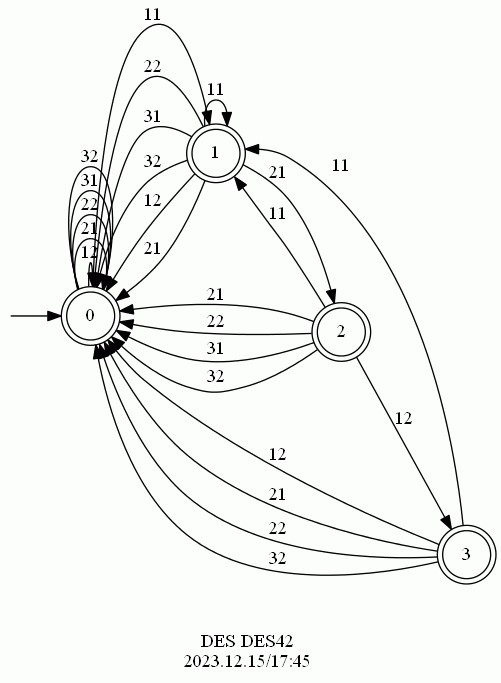
\includegraphics[width=0.6\linewidth]{assets/DES42.jpg}
  \caption{Homework42}
  \label{fig:des42}
\end{figure}

Figure \ref{fig:des42}, Evnets in the table \ref{tab:des42}

\section{Suppose that a plant $G$ has its alphabet $\Sigma=\left\{a_1, a_2, b_1, b_2, g_1, g_2\right\}$. Build another automaton that will generate the sublanguage of $L(G)$ where all the strings in $L(G)$ that contains the substrings $a_1 a_2 b_2$ or $a_1 a_2 g_2$ are removed.}

\paragraph{Answer}:
%43
wait

\begin{table}
  \centering
  \begin{tabular}{|c|c|}
    $a_1$ & 11\\
    $a_2$ & 12\\
    \hline
    $b_1$ & 21\\
    $b_2$ & 22\\
    \hline
    $g_1$ & 31\\
    $g_2$ & 32\\
  \end{tabular}
  \caption{Homework43}
  \label{tab:des43}
\end{table}

\begin{figure}
  \centering
  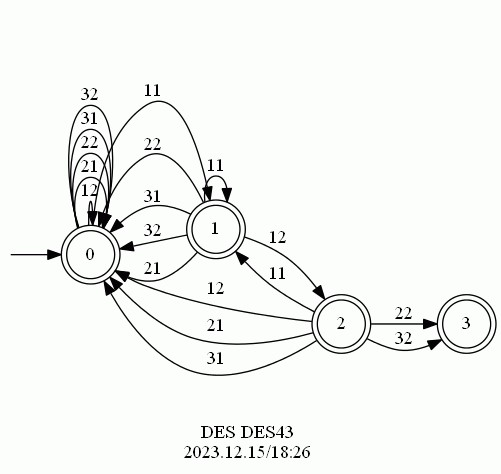
\includegraphics[width=0.6\linewidth]{assets/DES43.jpg}
  \caption{Homework43}
  \label{fig:des43}
\end{figure}

Figure \ref{fig:des43}, Evnets in the table \ref{tab:des43}


\section{Consider a plant $G$ with $L(G)=a^* b^*$ and the prefix-closed admissible language}

Consider a plant $G$ with $L(G)=a^* b^*$ and the prefix-closed admissible language is
$$
L_a=\left\{a^n b^m \mid n \geq m \geq 0\right\}
$$
Let the set of uncontrollable events be $E_{u c}=\{a\}$. Check if $L_a$ is controllable and if it is a regular language.

\paragraph{Answer}:
%44

Take into account any finite length string $s \in \bar{L_a}\Sigma_{uc} \cap L(G)$. String s takes the form of $s = a^n$ for some $n \in \mathbb{N}$ sine any string of the form $a^jb^k(j \in \mathbb{N}, k \geq 1)$ does not belong to $\bar{L_a}\Sigma_{uc}$. This means that $s^n$ belongs to $\bar{L_a}$. That is, $L_a$ is controllable.

$L_a$ requires to memorize how many times event $a$ happens to decide the number of allowed events of $b$ after a substring of $a\prime s$. Due to this required counting, $L_a$ is not regular (recall the definition of regular languages).

\section{Given a plant $G$ with $\Sigma_{u c} \subseteq \Sigma$ being the set of uncontrollable events and $K \subseteq \Sigma^*$.}
 
Given a plant $G$ with $\Sigma_{u c} \subseteq \Sigma$ being the set of uncontrollable events and $K \subseteq \Sigma^*$.Show the definition of controllability is equivalent to
$$
\bar{K} \Sigma_{u c}^* \cap L(G) \subseteq \bar{K}
$$

\paragraph{Answer}:
%45
We know the defination of controllable Let $K \subseteq \Sigma^*(K=\emptyset)$. K is controllable with respect to $\mathrm{G}$ if
$$
\begin{array}{r}
\bar{K} \Sigma_u \cap L(G) \subseteq \bar{K} \\
\bar{K} \Sigma_u=\left\{s \in \Sigma^* \mid s=s^{\prime} \sigma, \sigma \in \Sigma_u, s^{\prime} \in K\right\}
\end{array}
$$
Equivalently, $\left(\forall s \in \Sigma^*\right)(\forall \sigma \in \Sigma) s \in K$ and $\sigma \in \Sigma_u$ and $s \sigma \in L(G) \Rightarrow s \sigma \in$
$K$
For exmple $L_1=\{\alpha \lambda \mu\}$ and $\overline{L_1}=\{\varepsilon, \alpha, \alpha \lambda, \alpha \lambda \mu\}$. $L_1$ is uncontrollable since $s=\alpha \in \bar{K}, \beta \in \Sigma_u, \alpha \beta \in L(G)[\alpha \beta \notin \bar{K}]$. For $s=\alpha, \sigma=\beta$ or $\lambda$
Test $\lambda: \lambda \alpha \in K\left(\lambda \in \Sigma_u\right)$ controllable
Test $\beta: \alpha \beta \notin L_1$ uncontrollable. Thus $L_1$ is uncontrollable.


\section{Check the possibility that we can always construct a supervisor $S$ for a plant $G$ such that}
(a) $L(S / G)=L(G)$,(b) $L(S / G)=L_m(G)$, (c) $L(S / G)=\emptyset$, (d) $L(S / G)=\{\varepsilon\}$, and (e) $L_m(S / G)=\emptyset$.


\paragraph{Answer}:
%46
\begin{itemize}
  \item[(a)] True, taking $S(s) = \Sigma$ for any $s \in L(G)$.
  \item[(b)] False, we need that $L_m(G)$ is prefix-closed and controllable. 
  \item[(c)] False, as $L(S|G)$ is not empty.
  \item[(d)] False, $\{\epsilon\}$ needs to be controllable.
  \item[(e)] False, we need to have K such that $K \subseteq L(G)$, $K$ is controllable, and $K \cap L_m(G) = \emptyset$. 
\end{itemize}

\section{Consider the automata $G$ and $H$ as shown. Let $\Sigma_{uc} = \{d\}$.}
(a) Find all the controllable sublanguage of $L(H)$ with respect to $G$ and $\Sigma_{u c}$.

(b) Find all the controllable sublanguage of $L_m(H)$ with respect to $G$ and $\Sigma_{u c}$.

\paragraph{Answer}:
%47

$L(H)=\{ \epsilon, a(bcb)*, bc, ba(cbb)* \}$



\section{(Controllability test of language) There is a procedure to test the controllability of a language.}
\begin{enumerate}
  \item Suppose that $K$ and $L(G)$ are regular.
  \item Let $H$ be an automaton that generates $K$ and $G$ be an automaton that generates $L(G)$. Controllability can be checked by comparing the active event set of each state of $H \times G$ with the feasible event set of the corresponding state of $G$ (given by the second component of the state of $H \times G$ ).
  \item If there is an uncontrollable event in the latter that does not appear in the former, then $K$ is not controllable.
  \item The worst-case computational complexity of this test is $\mathcal{O}(|E| m n)$, where $m$ is the number of states of $H$ and $n$ is the number of states of $G$.
\end{enumerate}


\paragraph{Answer}:
%48
Proof We know the defination of controllable Let $K \subseteq \Sigma^*(K=\emptyset)$. $K$ is controllable with respect to $\mathrm{G}$ if
$$
\begin{array}{r}
\bar{K} \Sigma_u \cap L(G) \subseteq \bar{K} \\
\bar{K} \Sigma_u=\left\{s \in \Sigma^* \mid s=s^{\prime} \sigma, \sigma \in \Sigma_u, s^{\prime} \in K\right\}
\end{array}
$$
Equivalently, $\left(\forall s \in \Sigma^*\right)(\forall \sigma \in \Sigma) s \in K$ and $\sigma \in \Sigma_u$ and $s \sigma \in L(G) \Rightarrow s \sigma \in$
$K$
For exmple $L_1=\{\alpha \lambda \mu\}$ and $\overline{L_1}=\{\varepsilon, \alpha, \alpha \lambda, \alpha \lambda \mu\}$. $L_1$ is uncontrollable since $s=\alpha \in \bar{K}, \beta \in \Sigma_u, \alpha \beta \in L(G)[\alpha \beta \notin \bar{K}]$. For $s=\alpha, \sigma=\beta$ or $\lambda$
Test $\lambda: \lambda \alpha \in K\left(\lambda \in \Sigma_u\right)$ controllable
Test $\beta: \alpha \beta \notin L_1$ uncontrollable. Thus $L_1$ is uncontrollable.


\section{(Supervisor realization for a controllable language) Supervisor realization involves the computation of an automaton (generator) to represent a controllable language. Typically and conventionally, we consider two cases: $K=\bar{K} \subseteq L(G)$ and $K \subseteq L_m(G)$ with $K \neq \emptyset$}
\paragraph{Question} Propose a controllable language $K$ for a plant $G$ with $K = \bar{K} \subseteq L(G)$ and $K \neq  \emptyset$ and find its realization. Repeat the above for a plant and a non-empty language $K \subseteq L_m(G)$

\paragraph{Answer}:
%49


Let $G$ be a DES with $\Sigma=\{\alpha, \beta, \mu, \lambda\}$, where $\alpha:=11, \beta:=22, \mu:=$ $33, \lambda:=44 . \Sigma_o=\{\mu\}$, and $K=\{\alpha \mu, \beta \alpha\} \subseteq L_m(G)$. Naturally, we have $B=\{(1,1),(2,2)\}$. For For boundary state $(1,1), T(1,1)=\{b\}$ and $\Sigma(1,1)=$ $\{\mu\}$. Then $P^{-1} P[T(1,1)] \Sigma(1,1) \cap \bar{K}=\{\alpha, \beta, \lambda\}^*\{\mu\} \cap\{\alpha \mu, \beta \alpha\}=\{\alpha \mu, \beta \mu\} \cap$ $\{\alpha \mu, \beta \alpha\}=\{\alpha \mu\} \neq \emptyset . G=\operatorname{Meet}\{G 1, G 2\}$

\section{A cat and a mouse are placed in a maze with five rooms. Each door in a room is exclusively for either the cat or the mouse and can be used only in the direction indicated. Initially, the cat is in Room 3 and the mouse in Room 5. To help us understand the behavior of cat and mouse, we propose here their models by Petri nets. Actually, a transition (graphically represented by a bar) between two places (pictorially visualized by cycles) denotes a transition of an automaton. Specifically, in a Petri net model, a place can be regarded as a state of an automaton. The movement of the cat or mouse is done along the directed arrows in its Petri net model. Accordingly its automaton model can be constructed by treating a place (cycle) of the Petri net as a state while a related transition is treated as an event. Then, the model of cat has five states and that of mouse has the same number of states. With the help of these hints, try to solve the following questions (hint: TCT procedure mutex($q_1$, $q_2$) will be used).}

\begin{enumerate}
  \item Model the cat $(C)$ and mouse $(M)$ as finite state automata and compute the plant $G=C \| M$.
  \item It is required that the cat and mouse can never share a room and the cat and the mouse can return to their initial rooms. From plant $G$, identify the an automaton that satisfies the requirements.
  \item Find a supervisor using TCT assuming that all the events are controllable.
  \item Propose a number of different pairs of $\left(\Sigma_c, \Sigma_u\right)$ and find their corresponding supremal controllable sublanguages using TCT.
  \item Suppose that there are two cats. Repeat (1)-(4) as above (note that the Petri net modeling philosophy remains helpful to create the automaton model of multiple cats or mouses).
\end{enumerate}

\paragraph{Answer}:
%50


%...
\begin{figure}[h!]
  \centering
  \begin{subfigure}[b]{0.4\linewidth}
    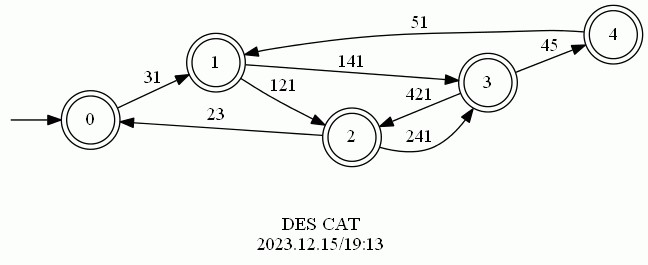
\includegraphics[width=\linewidth]{assets/CAT.jpg}
     \caption{Cat.}
  \end{subfigure}
  \begin{subfigure}[b]{0.4\linewidth}
    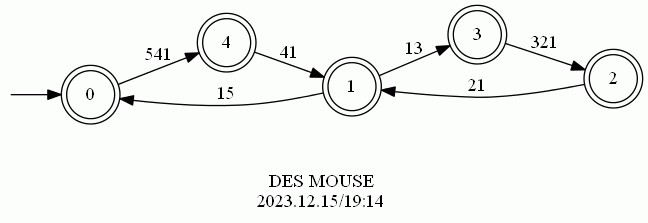
\includegraphics[width=\linewidth]{assets/MOUSE.jpg}
    \caption{Mouse.}
  \end{subfigure}
  \begin{subfigure}[b]{\linewidth}
    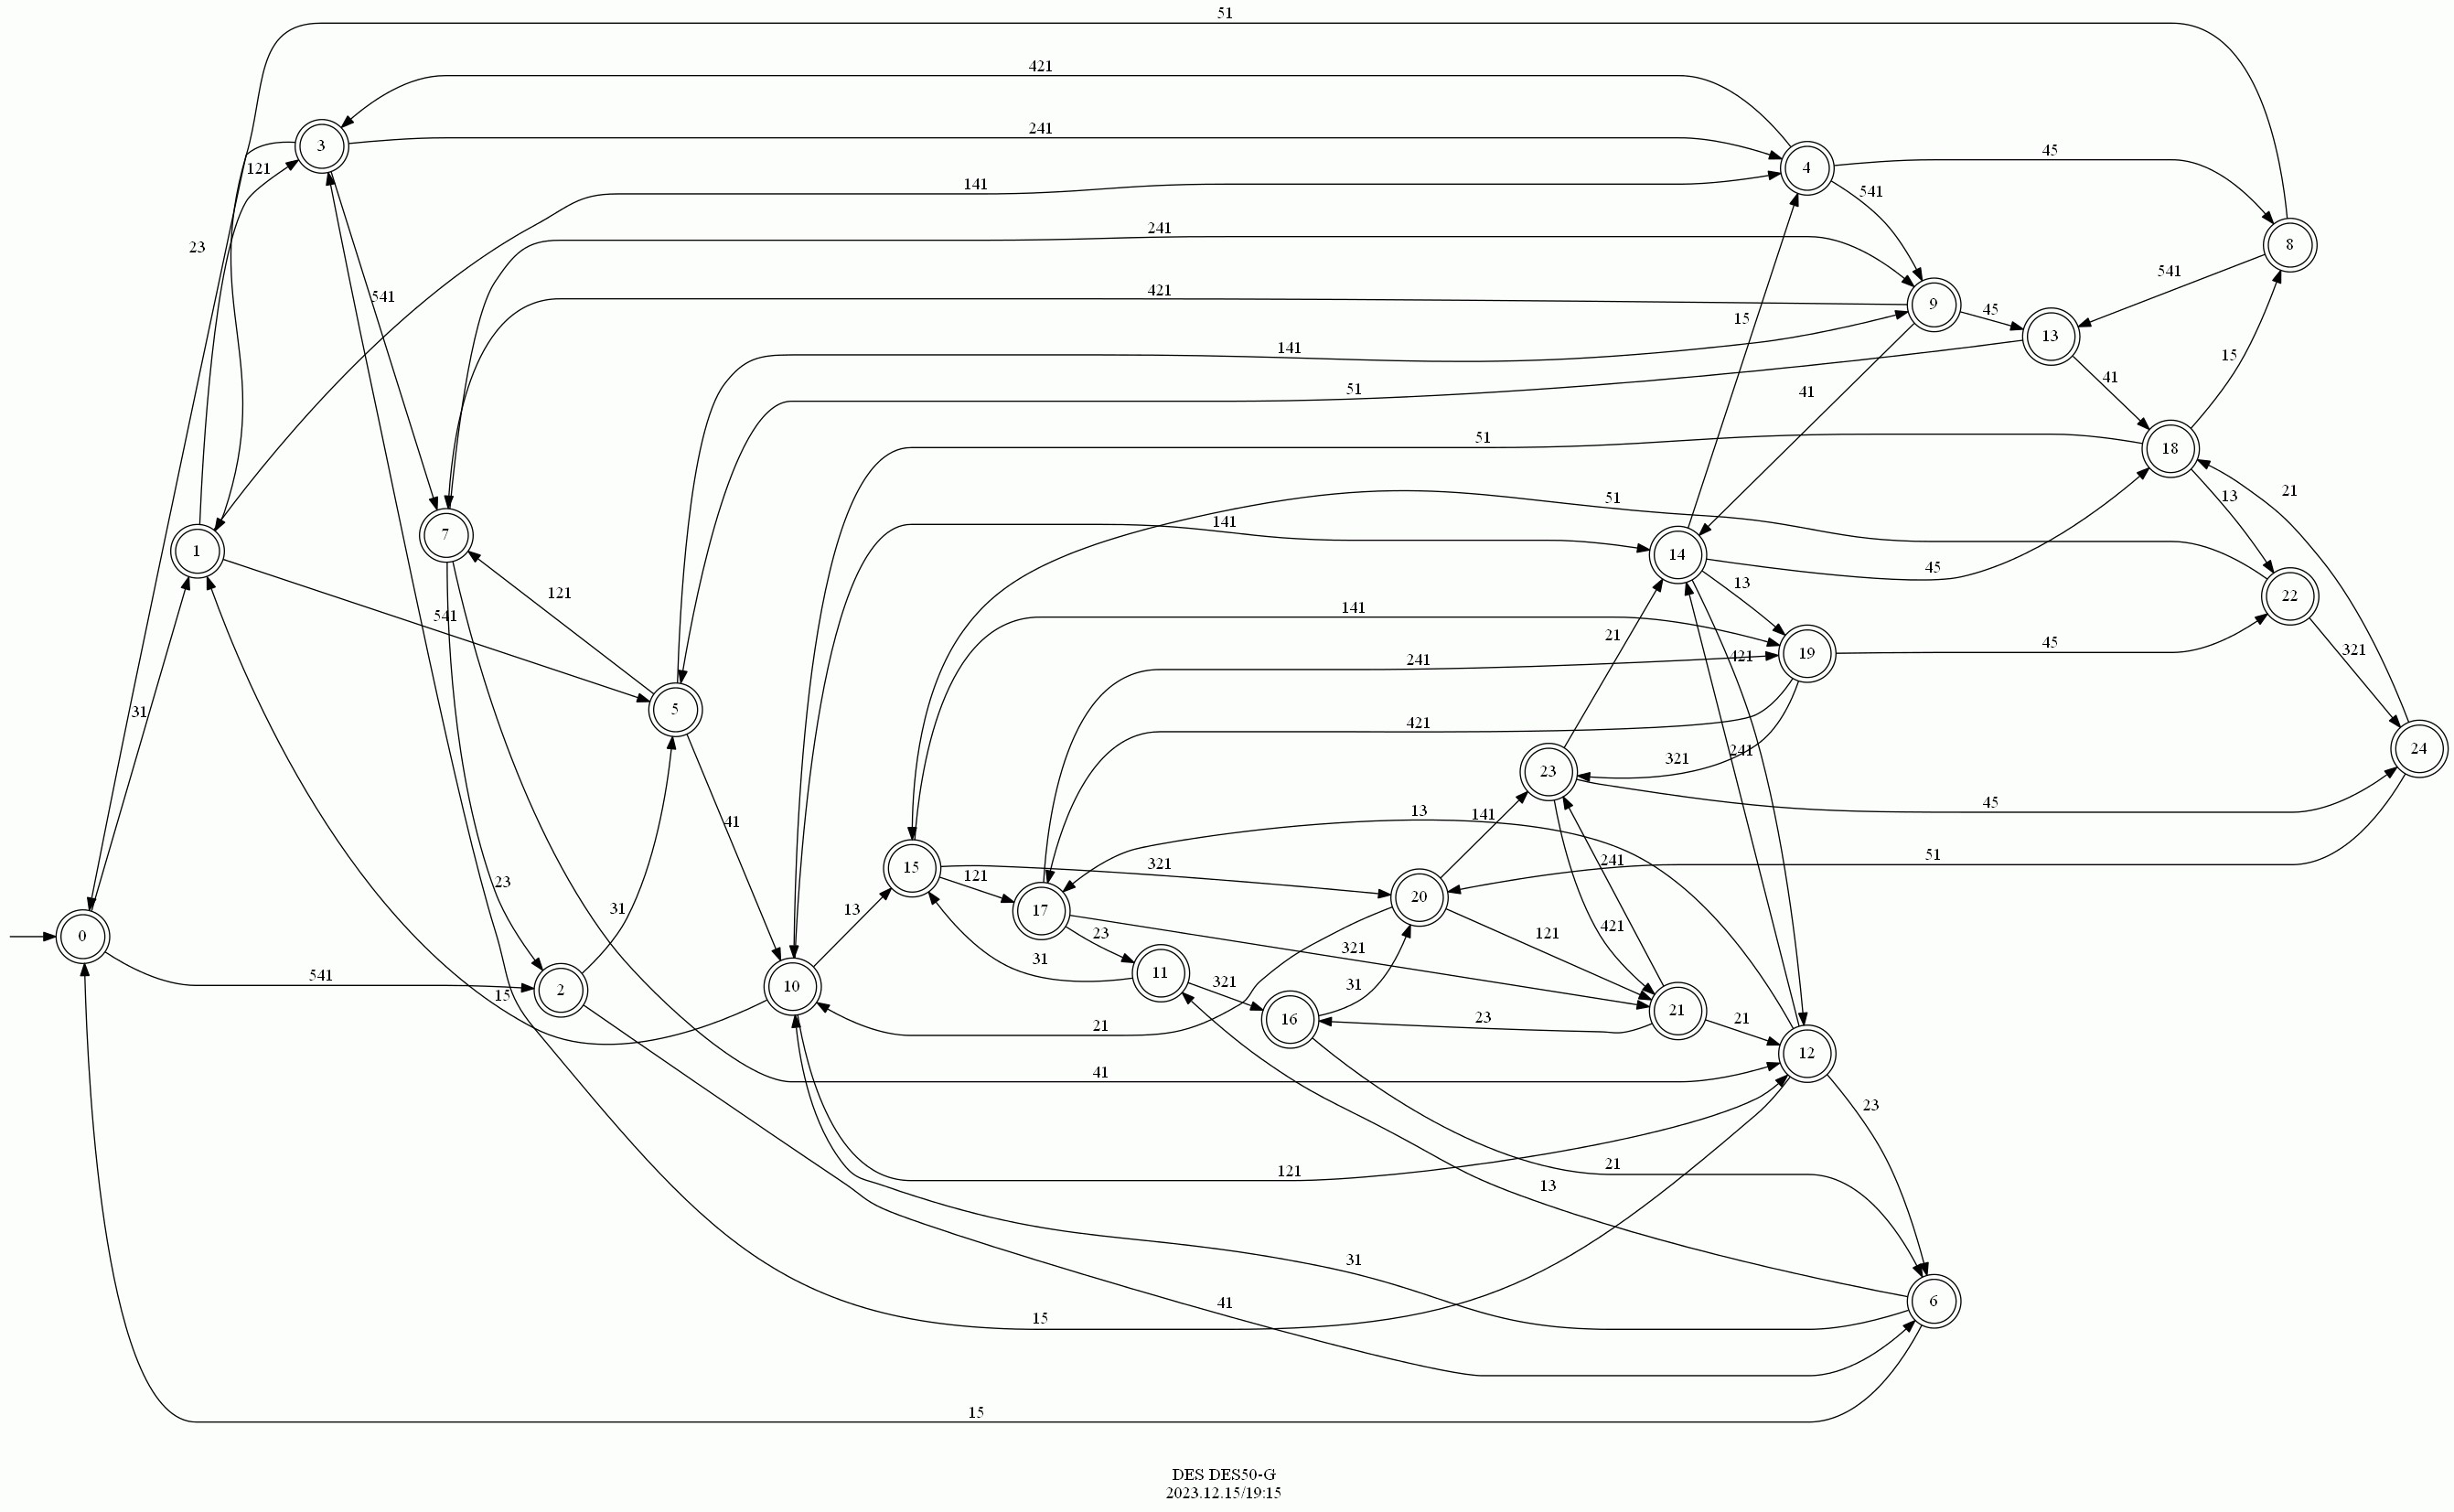
\includegraphics[width=\linewidth]{assets/DES50-G.jpg}
    \caption{G.}
  \end{subfigure}
  \begin{subfigure}[b]{0.8\linewidth}
    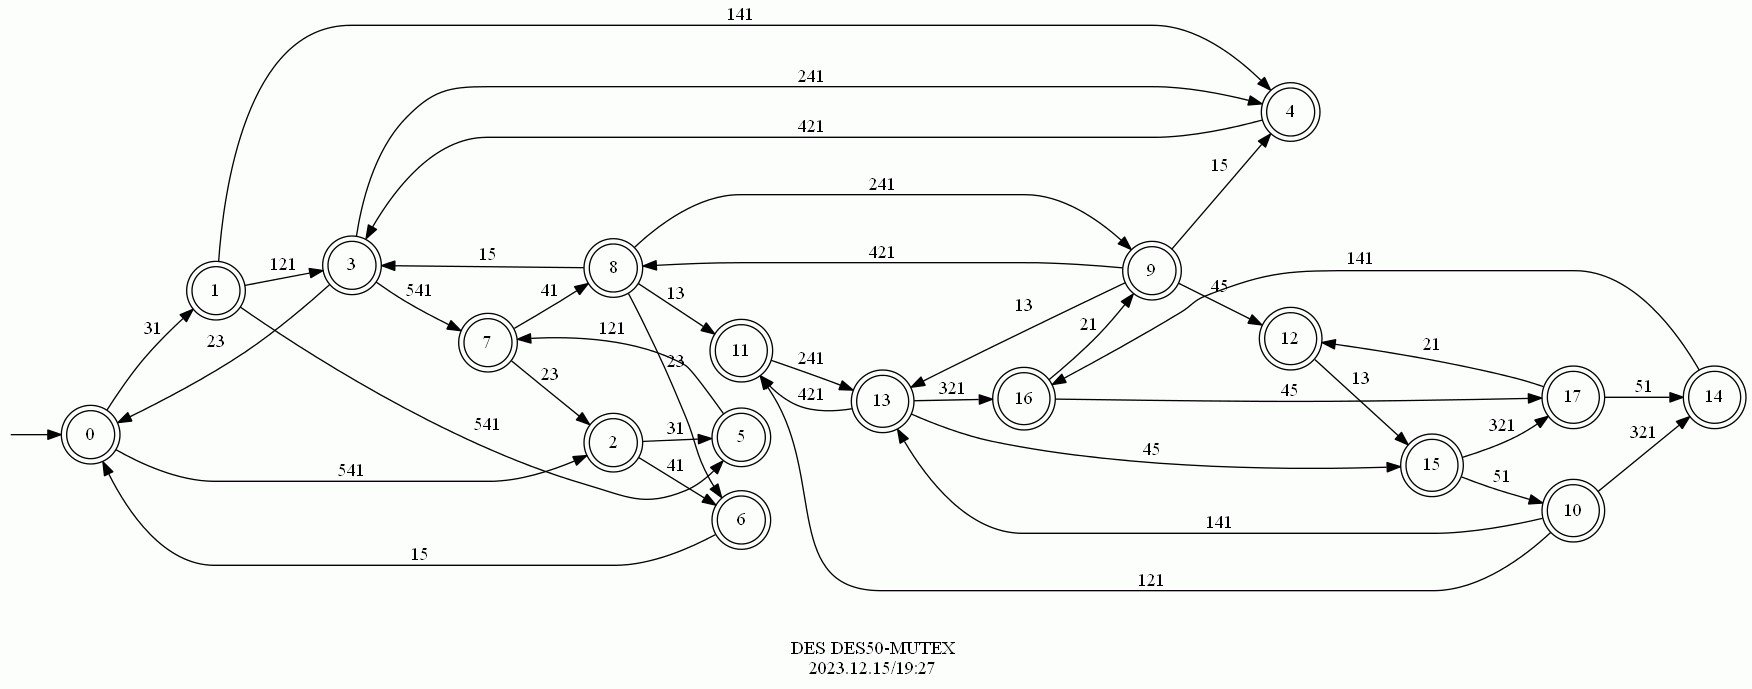
\includegraphics[width=\linewidth]{assets/DES50-MUTEX.jpg}
    \caption{Mutex.}
  \end{subfigure}
  \caption{homework50.}
  \label{fig:des50}
\end{figure}

Figure \ref{fig:des50}


\section{Consider the Small Factory consisting of two machines M1 and M2 and a buffer with capacity}

\paragraph{Question} Let us now consider another control specification. Let K2 be the admissible language corresponding to the specification that if both machines break down, M2 should be repaired first. Find K2 using TCT and check its controllability.

\paragraph{Answer}:
%51
wait

\section{Given a plant $G$ with alphabet $\Sigma^*$ and a control specification (language) $E$, sup($E$) is the supremal controllable language with respect to $G$ and $E$}

\paragraph{Question 6.} Show $\sup \left(E_1\right) \subseteq \sup \left(E_2\right)$ if $E_1 \subseteq E_2$ (monotonicity of supremal controllable sublanguages).
\paragraph{question 7.} Show sup($E$) is prefix-closed if $E$ is prefix-closed.
\paragraph{question 8.} Show the following properties pertaining to the supremal controllable sublanguage.
\paragraph{Proposition 1} (Properties of supremal controllable sublanguage).
\begin{enumerate}
  \item $sup(E_1 \cap E_2) \subseteq sup(E_1) \cap sup(E_2)$;
  \item $sup(E_1 \cap E_2) = sup(sup(E_1) \cap sup(E_2))$;
  \item $sup(E_1 \cap E_2) = sup(E_1) \cap sup(E_2)$ if $E_1$ and $E_2$ are not conflicting (trivially true if $E_1$ and $E_2$ are prefix-closed).
  \item $sup(E_1 \cup E_2) \subseteq sup(E_1 \cup E_2)$
\end{enumerate}


\paragraph{Answer}:
%52

wait


\section{Given a control specification $E \subseteq L(G)$ for some $G$ with $L(G) \subseteq \Sigma^*$, we define the class of prefix-closed and controllable superlanguages of $E$}

\paragraph{Question 9.} Question 9. Show that $\inf (E) \in \arg (E)$ and $\inf (E)$ is controllable.

In the worst case, $\inf (E)=L(G)$ since $L(G) \in \arg (E)$. If $E$ is controllable, $\inf (E)=\bar{E}$.

\paragraph{Question 10.} Show the following properties.

\begin{enumerate}
  \item  $E_1 \subseteq E_2 \Longrightarrow \inf \left(E_1\right) \subseteq \inf \left(E_2\right)$;
  \item $\inf \left(E_1 \cap E_2\right) \subseteq \inf \left(E_1\right) \cap \inf \left(E_2\right)$;
  \item $\inf \left(E_1 \cup E_2\right)=\inf \left(E_1\right) \cup \inf \left(E_2\right)$.
\end{enumerate}

\paragraph{Answer}:
%53

wait

\section{Let $\Sigma=\{\alpha, \beta, \lambda, \mu\}, \Sigma_o=\{\alpha, \beta\}, L(G)=\overline{\{\alpha, \beta, \lambda \alpha, \mu \alpha\}}, K=\overline{\{\alpha, \lambda \alpha\}}$. Verify that $K$ is observable with respect to $L(G), \Sigma_o$, and $\Sigma_c=\Sigma$}

\paragraph{Answer}:
%54

Proof $\Sigma=\{\alpha, \beta, \lambda, \mu\}, \Sigma_o=\{\alpha, \beta\}$ $L(G)=\overline{\lambda \alpha+\mu(\alpha+\beta)}$. Let $K=\overline{\lambda \alpha+\mu \beta} . \quad K=\{\varepsilon, \lambda, \mu, \lambda \alpha, \mu \beta\}=\bar{K}$ (prefix-closed). Check $(\varepsilon, \lambda),(\varepsilon, \mu)$, and $(\lambda, \mu) . K$ is closed, so condition (2) is dropped.

\begin{enumerate}
  \item  $s=\varepsilon, s^{\prime}=\lambda$. Check $\sigma=\lambda$ or $\mu(\varepsilon \alpha, \varepsilon \beta \notin \bar{K})$. Note that $s^{\prime} \sigma=\lambda \lambda \notin L(G)$ and $s^{\prime} \sigma=\lambda \mu \notin L(G)$. Thus, $(\varepsilon, \lambda) \in a^{\prime c} t_K$.
  \item $s=\varepsilon, s^{\prime}=\mu$. Check $\sigma=\lambda$ or $\mu(\varepsilon \alpha, \varepsilon \beta \notin \bar{K})$. Note that $s^{\prime} \sigma=\mu \lambda \notin L(G)$ and $s^{\prime} \sigma=\mu \mu \notin L(G)$. Thus, $(\varepsilon, \mu) \in a^{\prime} t_K$.
  \item $s=\lambda, s^{\prime}=\mu$. Check $\sigma=\alpha(\lambda \mu, \lambda \lambda, \lambda \beta \notin \bar{K})$. Note that $s \sigma=\lambda \alpha \in K$, $s^{\prime} \sigma=\mu \alpha \in L(G)$ but $s^{\prime} \sigma=\mu \alpha \notin \bar{K}$. Thus, $(\lambda, \mu) \notin$ act ${ }_K$.
\end{enumerate}

Suppose $L_m(G)=\varepsilon+\lambda(\varepsilon+\alpha)+\mu(\alpha+\beta), J=\varepsilon+\lambda \alpha+\mu \beta$ Then $J=K$ but $J$ is not even $L_m(G)$-closed, since $\lambda \in \bar{J} \cap L_m(G), \lambda \notin J$ Now $\varepsilon \in J \cap L_m(G)$ and $\lambda \in J \cap L_m(G)$, but $\lambda \notin J$. so in this case $(\varepsilon, \lambda) \notin a c t_J$.

\section{Give an example of fixed $L(G), K, \Sigma_o$, and two different $\Sigma_c$ 's such that $K$ is observable with respect to the first choice of $\Sigma_c$ but not with respect to the second one.}

\paragraph{Answer}:
%55
The DES $G$ is following picture, where $a:=11, b:=22, c:=33, d:=44$ $\Sigma=\{a, b, c, d\}, \Sigma_o=\{a, c\}, \Sigma_c=\{a, c\}, \Sigma_u=\{b, d\}, L(G)=\{\varepsilon, a, a b, a b c, a d\}$. Let $K=\{a d, a b\}, \bar{K}=\{\varepsilon, a, a d, a b\}$.
Then $P^{-1} P \bar{K}=\{\varepsilon, a, a b, a d\}, L(G) \cap P^{-1} P \bar{K}=\{\varepsilon, a, a b, a d\}$
$\Longrightarrow \bar{K}=L(G) \cap P^{-1} P \bar{K}$
$\Longrightarrow \bar{K}$ is $(L(G), P)$-normal.
And we have $\bar{K} \Sigma_u \cap L(G) \subseteq \bar{K}, K$ is controllable. Let $s:=a b \in \bar{K}$ for $\sigma:=c \in \Sigma$, then $s \sigma:=a b c \in L(G)-\bar{K} \Longrightarrow \sigma \in \Sigma_o \cap \Sigma_c$.

\section{ Let $L(G)=\overline{\left\{u_1 a b, u_1 a g, u_2 a g\right\}}$ with  $\Sigma_c=\Sigma $ and $ \Sigma_{u o}=\left\{u_1, u_2\right\} $.}

\paragraph{Proof}:
%56 review
We know the defination of controllable Let $K \subseteq \Sigma^*(K=\emptyset)$. $\mathrm{K}$ is controllable with respect to $\mathrm{G}$ if
$$
\begin{array}{r}
\bar{K} \Sigma_u \cap L(G) \subseteq \bar{K} \\
\bar{K} \Sigma_u=\left\{s \in \Sigma^* \mid s=s^{\prime} \sigma, \sigma \in \Sigma_u, s^{\prime} \in K\right\}
\end{array}
$$
Equivalently, $\left(\forall s \in \Sigma^*\right)(\forall \sigma \in \Sigma) s \in K$ and $\sigma \in \Sigma_u$ and $s \sigma \in L(G) \Rightarrow s \sigma \in$
$K$
For exmple $L_1=\{\alpha \lambda \mu\}$ and $\overline{L_1}=\{\varepsilon, \alpha, \alpha \lambda, \alpha \lambda \mu\}$. $L_1$ is uncontrollable since $s=\alpha \in \bar{K}, \beta \in \Sigma_u, \alpha \beta \in L(G)[\alpha \beta \notin \bar{K}]$. For $s=\alpha, \sigma=\beta$ or $\lambda$
Test $\lambda: \lambda \alpha \in K\left(\lambda \in \Sigma_u\right)$ controllable
Test $\beta: \alpha \beta \notin L_1$ uncontrollable. Thus $L_1$ is uncontrollable.

\section{Consider the languages $L(G)=\overline{L(G)} \subseteq \Sigma^*$ and $L=\bar{L} \subseteq \Sigma_o^*$, where $P: \Sigma \rightarrow \Sigma_o$ is a natural projection. Let $\Sigma_{u c} \subseteq \Sigma$ be the set of uncontrollable events. Assume that $L \subseteq P[L(G)]$. Define the language}

$$
K=P^{-1}(L) \cap L(G)
$$

\begin{enumerate}
  \item Prove that $K$ is observable with respect to $L(G), \Sigma_o$, and $\Sigma$.
  \item Show that " $K$ is controllable with respect to $L(G)$ and $\Sigma_{u c}$ " if and only if " $L$ is controllable with respect to $P[L(G)]$ and $\Sigma_{u c} \cap \Sigma_o$."
\end{enumerate}

\paragraph{Answer}:
%57

The DES $G$ is following picture, where $a:=11, b:=22, c:=33, d:=44$ $\Sigma=\{a, b, c, d\}, \Sigma_o=\{a, c\}, \Sigma_c=\{a, c\}, \Sigma_u=\{b, d\}, L(G)=\{\varepsilon, a, a b, a b c, a d\}$. Let $K=\{a d, a b\}, \bar{K}=\{\varepsilon, a, a d, a b\}$.
Then $P^{-1} P \bar{K}=\{\varepsilon, a, a b, a d\}, L(G) \cap P^{-1} P \bar{K}=\{\varepsilon, a, a b, a d\}$
$\Longrightarrow \bar{K}=L(G) \cap P^{-1} P \bar{K}$
$\Longrightarrow \bar{K}$ is $(L(G), P)$-normal.
And we have $\bar{K} \Sigma_u \cap L(G) \subseteq \bar{K}, K$ is controllable. Let $s:=a b \in \bar{K}$ for $\sigma:=c \in \Sigma$, then $s \sigma:=a b c \in L(G)-\bar{K} \Longrightarrow \sigma \in \Sigma_o \cap \Sigma_c$.

\section{Consider the languages $K \subseteq L(G)=\overline{L(G)} \subseteq \Sigma^*$ and the natural projection $P: \Sigma \rightarrow \Sigma_o$. Show that the language
$$
P^{-1}[P(K)] \cap L(G)
$$
is observable with respect to $L(G), \Sigma_o$, and all choices $\Sigma_c \subseteq \Sigma$.}

\paragraph{Answer}:
%58

The DES $G$ is following picture, where $a:=11, b:=22, c:=33, d:=44$ $\Sigma=\{a, b, c, d\}, \Sigma_o=\{a, c\}, \Sigma_c=\{a, c\}, \Sigma_u=\{b, d\}, L(G)=\{\varepsilon, a, a b, a b c, a d\}$. Let $K=\{a d, a b\}, \bar{K}=\{\varepsilon, a, a d, a b\}$.
Then $P^{-1} P \bar{K}=\{\varepsilon, a, a b, a d\}, L(G) \cap P^{-1} P \bar{K}=\{\varepsilon, a, a b, a d\}$
$\Longrightarrow \bar{K}=L(G) \cap P^{-1} P \bar{K}$
$\Longrightarrow \bar{K}$ is $(L(G), P)$-normal.
And we have $\bar{K} \Sigma_u \cap L(G) \subseteq \bar{K}, K$ is controllable. Let $s:=a b \in \bar{K}$ for $\sigma:=c \in \Sigma$, then $s \sigma:=a b c \in L(G)-\bar{K} \Longrightarrow \sigma \in \Sigma_o \cap \Sigma_c$.

\section{Check the observability of a language using observer automata (Refer to Chapter 6B).}

\paragraph{Answer}:
%59

wait

\section{(Observability test) Observability checking using observer automata is subject to the computational complexity problem owing to the construction of an observer.}

\paragraph{Answer}:
%60

wait

\section{(Supervisor implementation under partial observation) We first tautologically present a result regarding the existence of a supervisor for a DES with partial observation.}

\paragraph{Answer}:
%61

wait

\section{Show that the property of normality is preserved under union and intersection.}

\paragraph{Answer}:
%62
MACH $=$ Create(MACH, $[\operatorname{mark} 0],[\operatorname{tran}[0,11,1],[1,10,0],[1,12,2],[2,13,0]])(3,4)$

ALLMACH $=$ allevent(MACH)

Nonconflicting(MACH, ALLMACH $)=$ True $\mathrm{MACH}$ is nonblocking.

\section{(Decentralized control problem) A system is usually subject to a number of control specifications.}

\paragraph{Answer}:
%63


\begin{figure}[h!]
  \centering
  \begin{subfigure}{0.26\linewidth}
    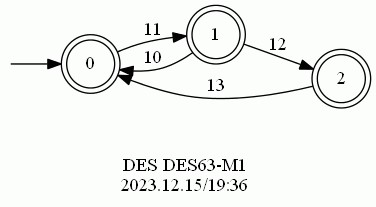
\includegraphics[width=\linewidth]{assets/DES63-M1.jpg}
     \caption{Machine1.}
  \end{subfigure}
  \begin{subfigure}{0.26\linewidth}
    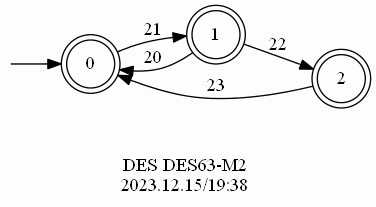
\includegraphics[width=\linewidth]{assets/DES63-M2.jpg}
     \caption{Machine2.}
  \end{subfigure}
  \begin{subfigure}{0.26\linewidth}
    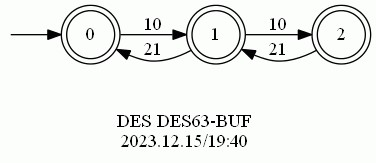
\includegraphics[width=\linewidth]{assets/DES63-BUF.jpg}
    \caption{BUF.}
  \end{subfigure}
  \begin{subfigure}{0.2\linewidth}
    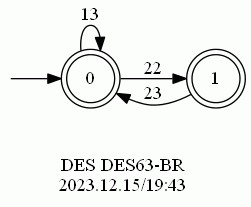
\includegraphics[width=\linewidth]{assets/DES63-BR.jpg}
    \caption{BR.}
  \end{subfigure}
  \begin{subfigure}{\linewidth}
    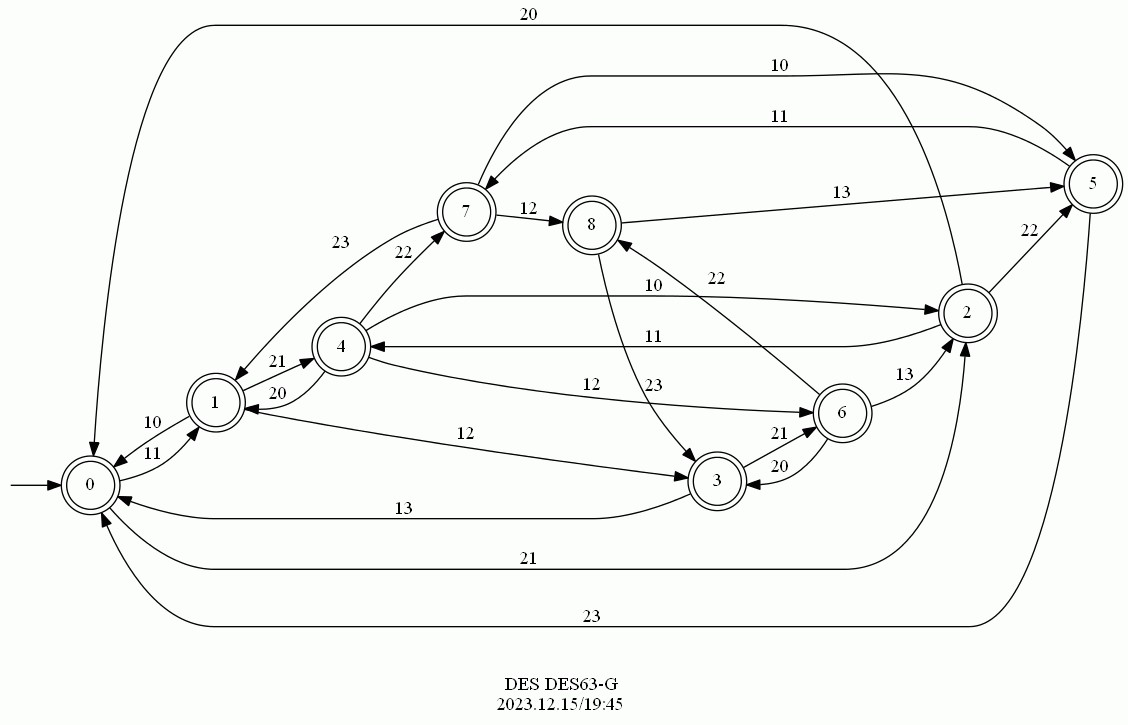
\includegraphics[width=\linewidth]{assets/DES63-G.jpg}
    \caption{G.}
  \end{subfigure}
  \caption{homework63.}
  \label{fig:des63}
\end{figure}

\begin{figure}[h!]
  \centering
  \begin{subfigure}{0.2\linewidth}
    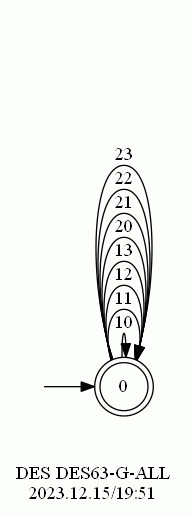
\includegraphics[width=\linewidth]{assets/DES63-G-ALL.jpg}
     \caption{G all.}
  \end{subfigure}
  \begin{subfigure}{0.3\linewidth}
    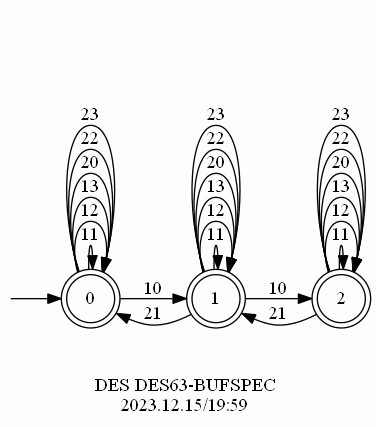
\includegraphics[width=\linewidth]{assets/DES63-BUFSPEC.jpg}
     \caption{BUF.}
  \end{subfigure}
  \begin{subfigure}{0.2\linewidth}
    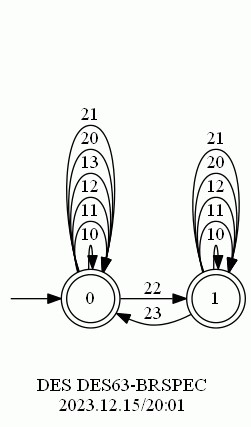
\includegraphics[width=\linewidth]{assets/DES63-BRSPEC.jpg}
    \caption{BR.}
  \end{subfigure}
  \begin{subfigure}{0.6\linewidth}
    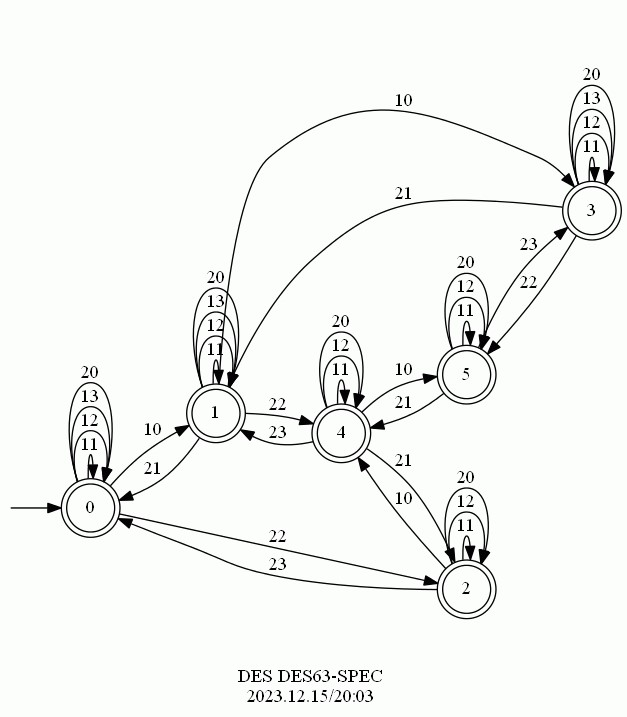
\includegraphics[width=\linewidth]{assets/DES63-SPEC.jpg}
    \caption{Spec.}
  \end{subfigure}
  \caption{homework63-spec.}
  \label{fig:des63-spec}
\end{figure}

\begin{figure}[h!]
  \centering
  \begin{subfigure}{0.6\linewidth}
    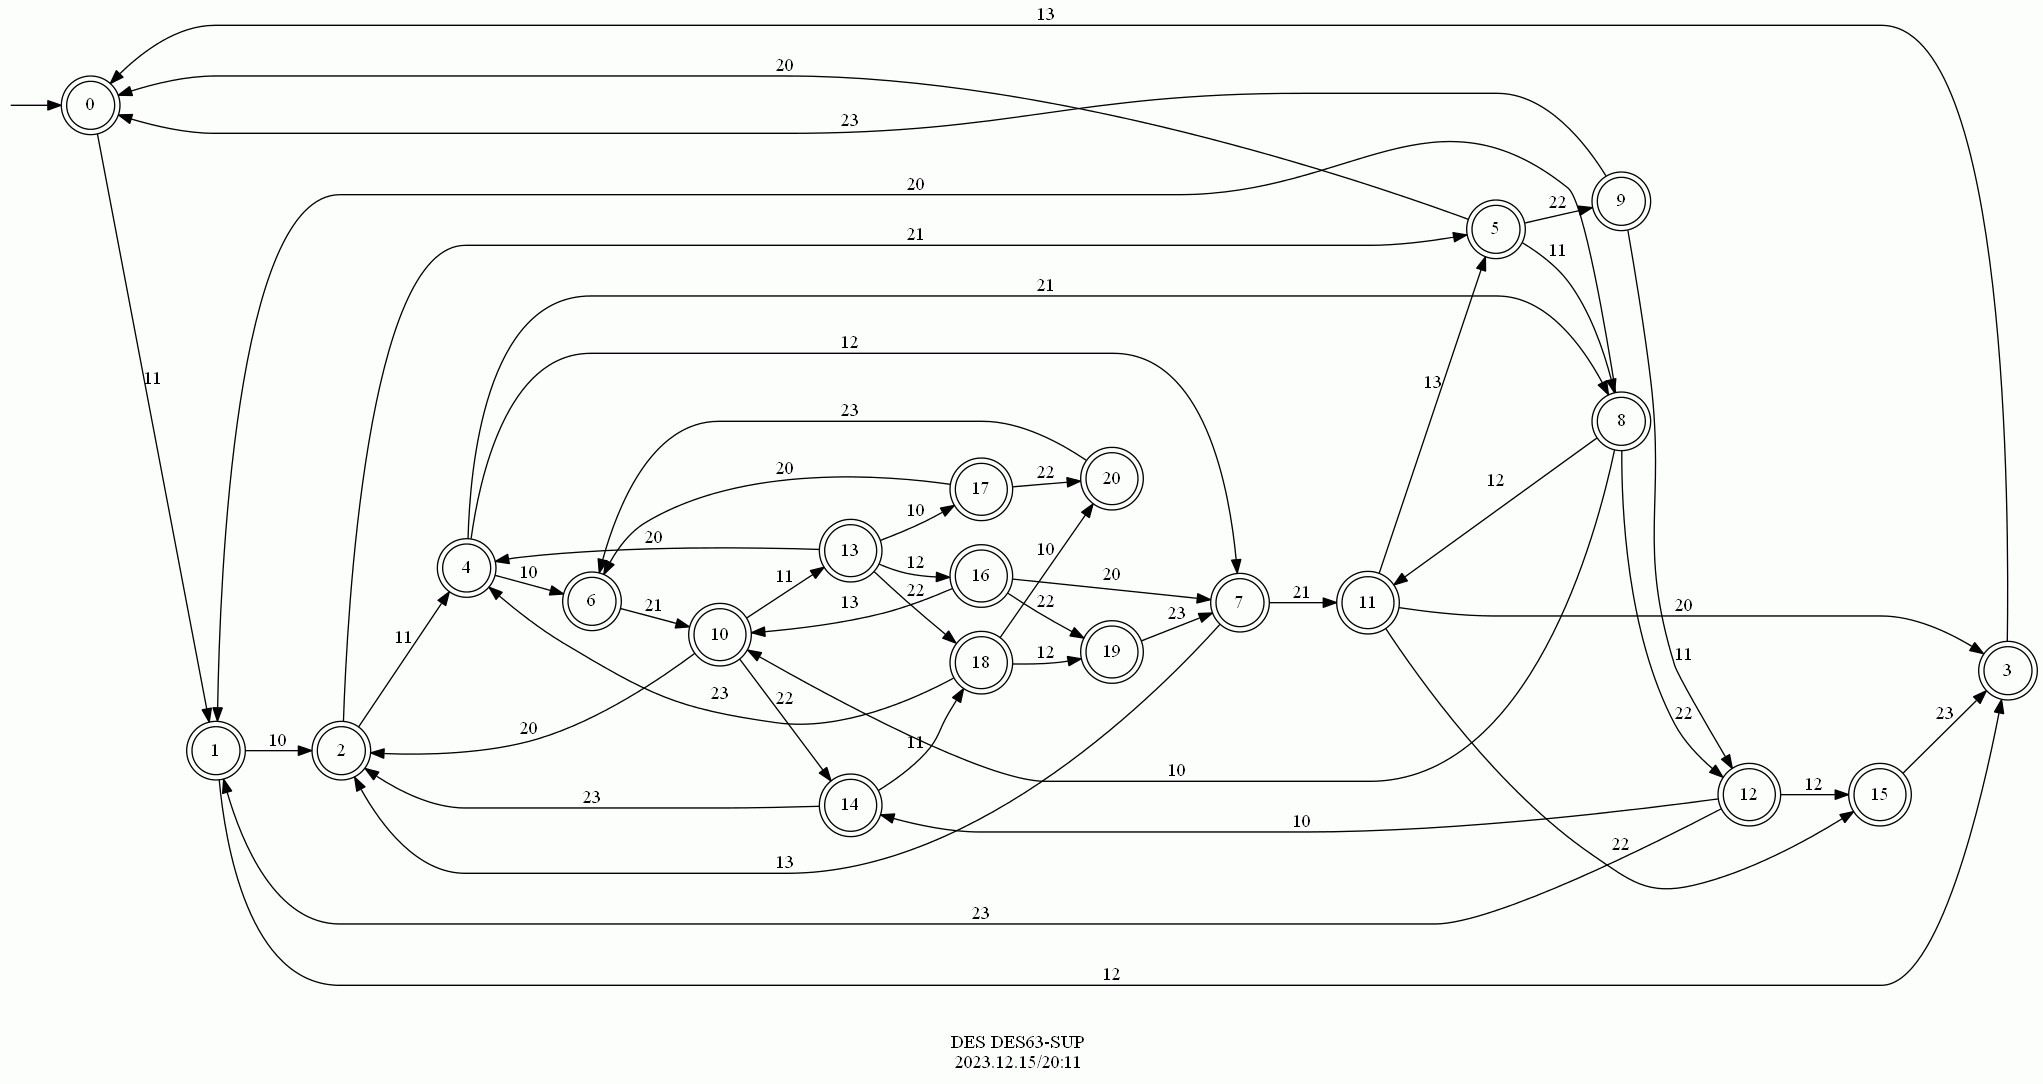
\includegraphics[width=\linewidth]{assets/DES63-SUP.jpg}
     \caption{SUP.}
  \end{subfigure}
  \begin{subfigure}{0.6\linewidth}
    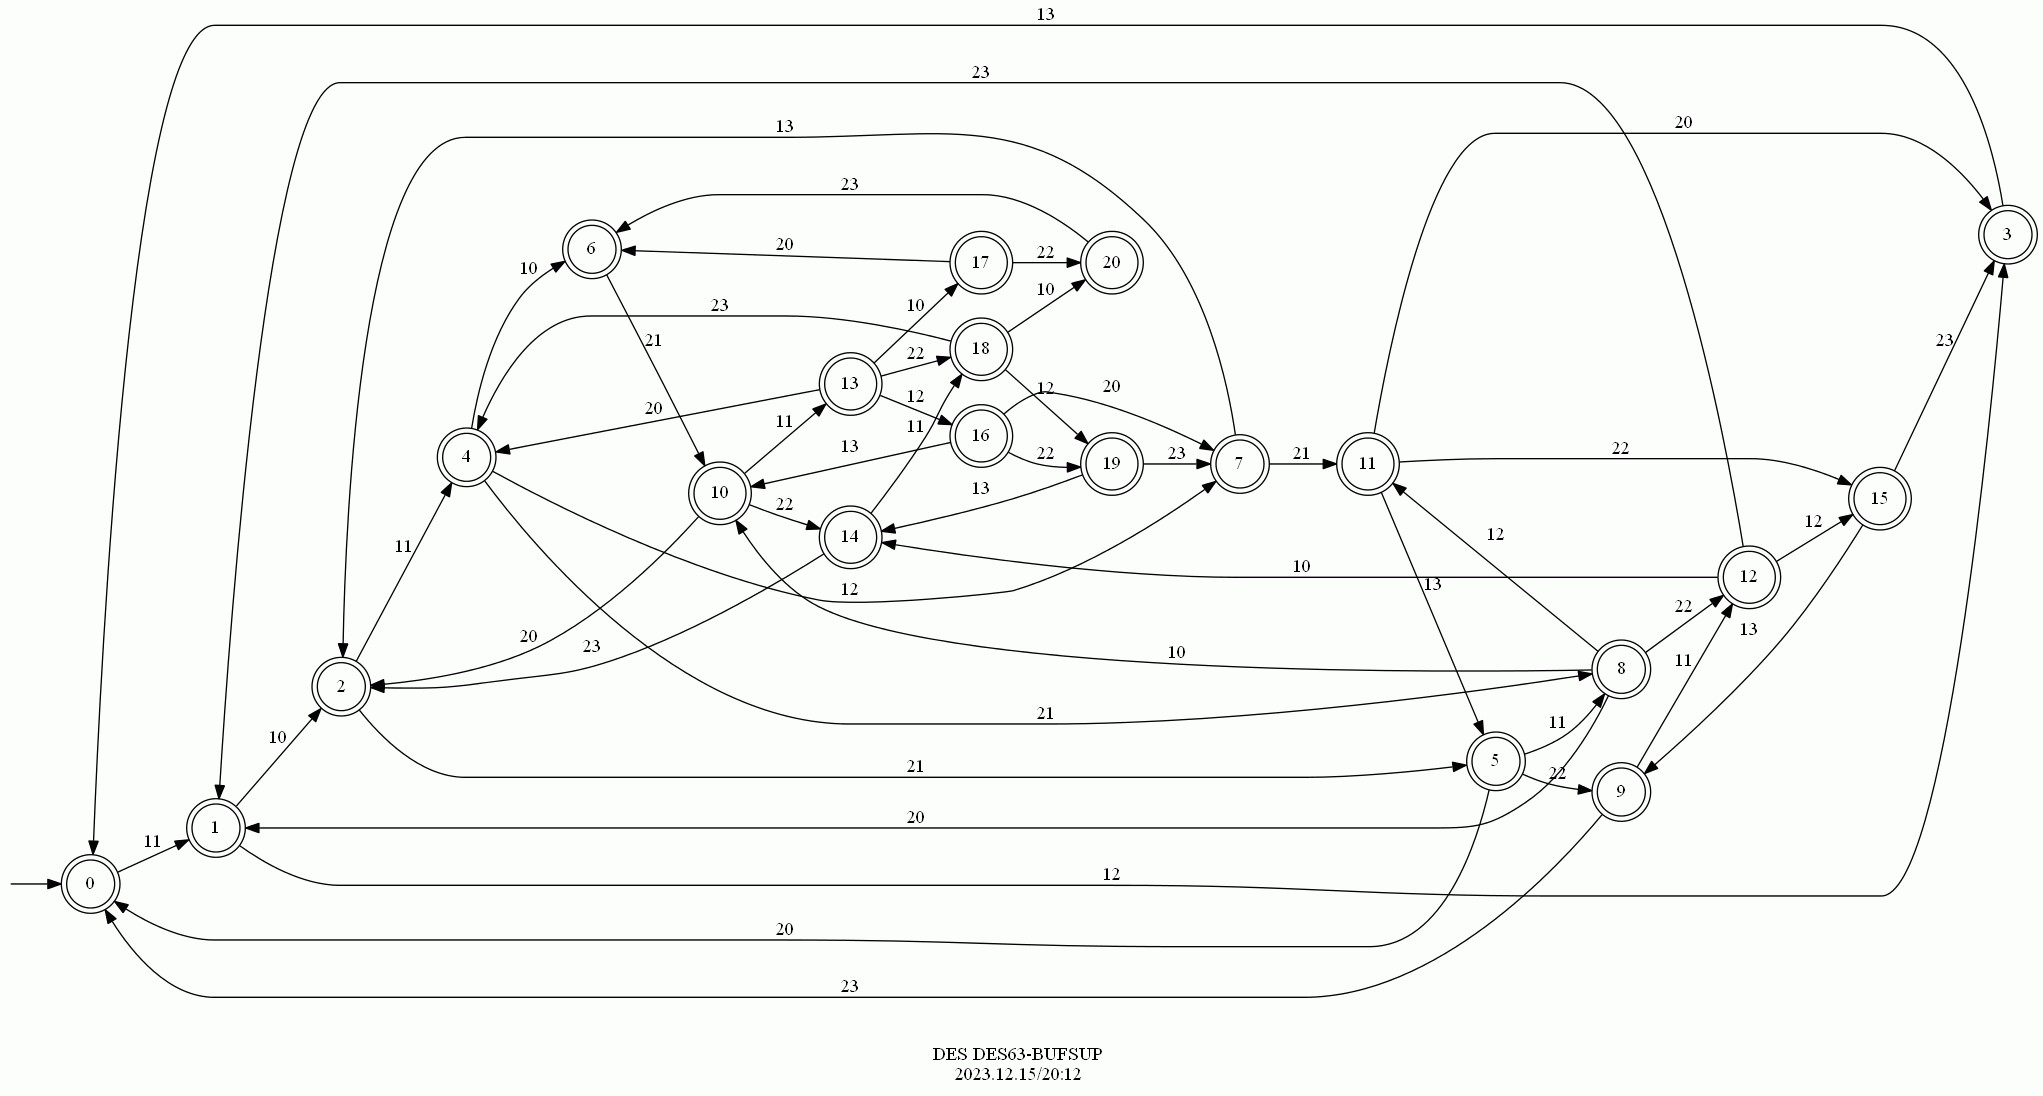
\includegraphics[width=\linewidth]{assets/DES63-BUFSUP.jpg}
     \caption{BUFSUP.}
  \end{subfigure}
  \begin{subfigure}{0.6\linewidth}
    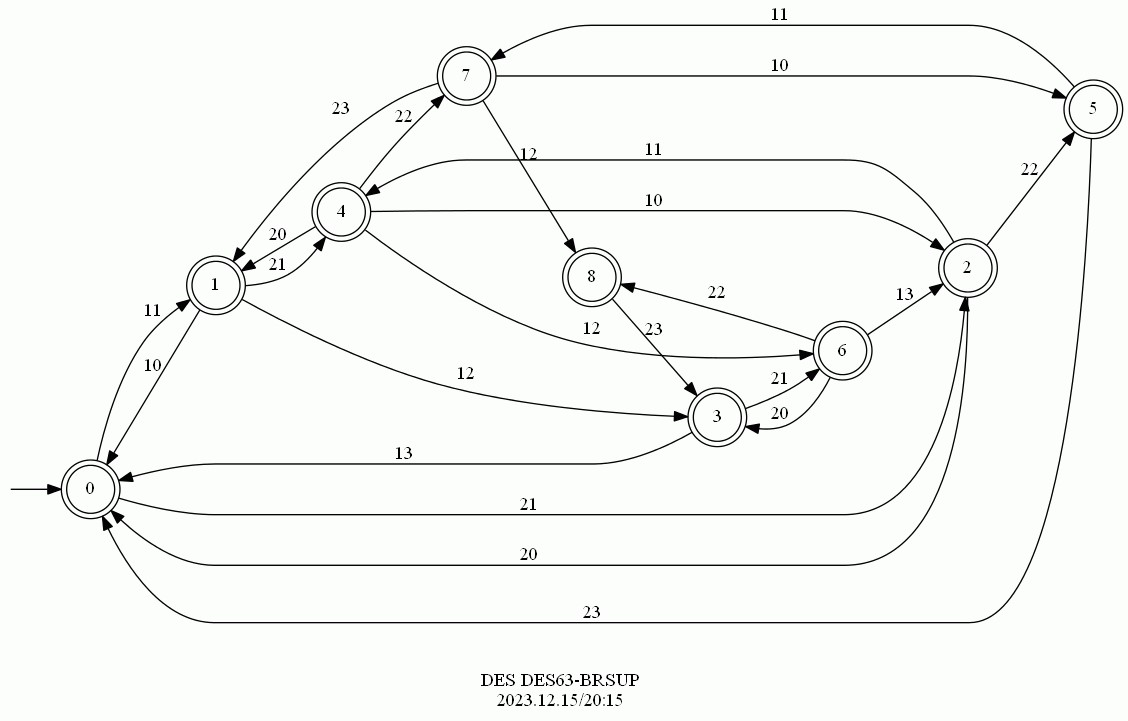
\includegraphics[width=\linewidth]{assets/DES63-BRSUP.jpg}
    \caption{BRSUP.}
  \end{subfigure}
  \caption{homework63-sup.}
  \label{fig:des63-sup}
\end{figure}


Figure \ref{fig:des63} shows G.

Figure \ref{fig:des63-spec} shows Spec.

Figure \ref{fig:des63-sup} shows SUP.





\section{(Decentralized control problem) Now let us consider another plant that is a manufacturing system consisting of two machines namely MACH 1 and MACH2, two buffers B1 and B2 with capacity 3 and 1, respectively, and a testing unit that will check the quality of the final products finished on MACH2.}

\paragraph{Answer}:
%64

repeat

\section{Use TCT to provide a solution to the missionaries and cannibals problem.}

\paragraph{Answer}:
%65

\begin{figure}
  \centering
  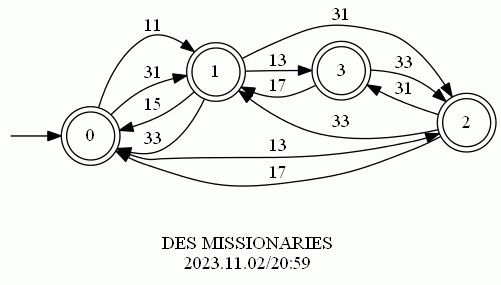
\includegraphics{assets/MISSIONARIES.jpg}
  \caption{Missionaries and Cannibals Problem}
  \label{fig:des65}
\end{figure}

As Figure \ref{fig:des65} shows.

\section{The Tower of Hanoi is a mathematical game or puzzle. It consists of three rods and a number of disks of different sizes, which can slide onto any rod. The puzzle starts with the disks in a neat stack in ascending order of size on one rod, the smallest at the top, thus making a conical shape.}

\paragraph{Answer}:
%66

wait


\section{Once upon a time a farmer went to a market and purchased a wolf, a goat, and a cabbage.}

\paragraph{Answer}:
%67

%...
\begin{figure}[h!]
  \centering
  \begin{subfigure}[b]{0.2\linewidth}
    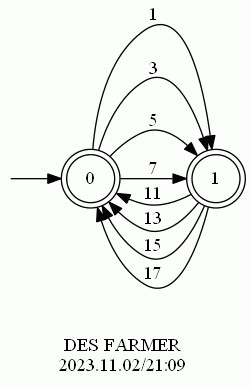
\includegraphics[width=\linewidth]{assets/FARMER.jpg}
     \caption{farmer.}
  \end{subfigure}
  \begin{subfigure}[b]{0.2\linewidth}
    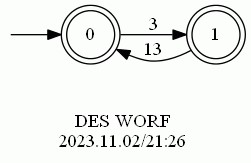
\includegraphics[width=\linewidth]{assets/WORF.jpg}
    \caption{wolf.}
  \end{subfigure}
  \begin{subfigure}[b]{0.2\linewidth}
    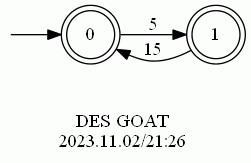
\includegraphics[width=\linewidth]{assets/GOAT.jpg}
    \caption{goat.}
  \end{subfigure}
  \begin{subfigure}[b]{0.2\linewidth}
    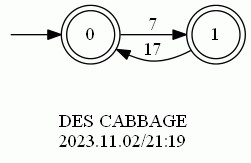
\includegraphics[width=\linewidth]{assets/CABBAGE.jpg}
    \caption{cabbage.}
  \end{subfigure}
  \begin{subfigure}[b]{\linewidth}
    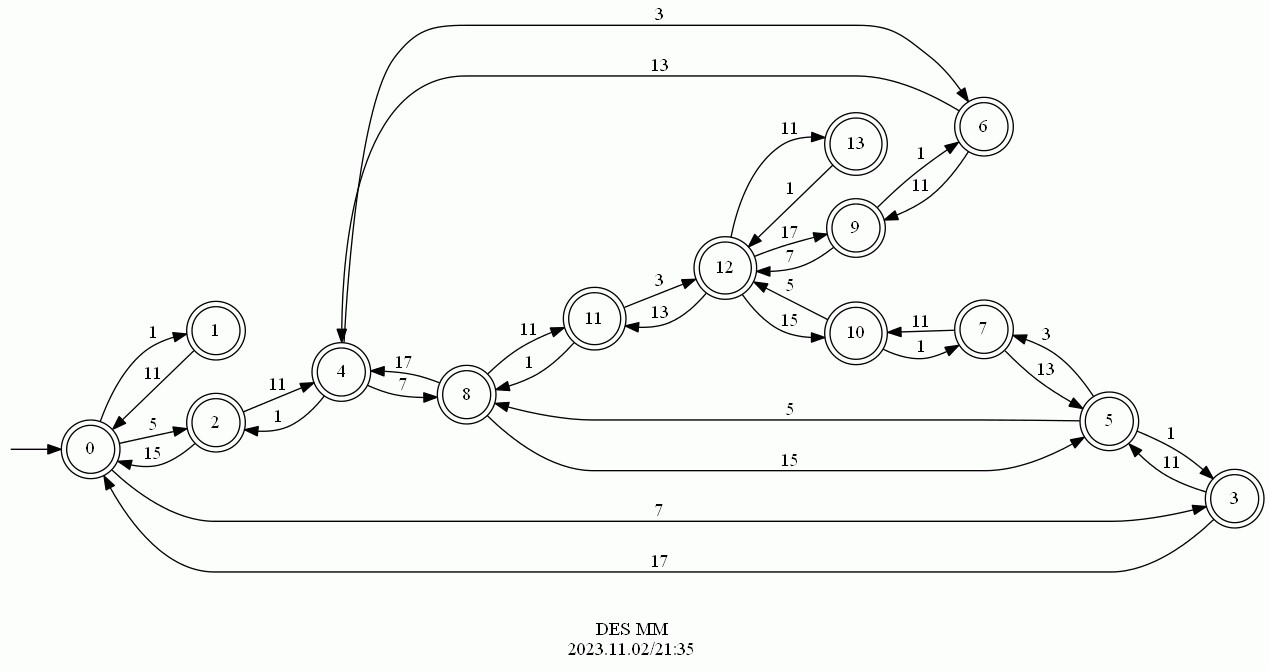
\includegraphics[width=\linewidth]{assets/DES67.jpg}
    \caption{crossing river.}
  \end{subfigure}
  \caption{DES67.}
  \label{fig:des67}
\end{figure}
%...

As Figure \ref{fig:des67} shows.


\section{Theorem: Let $K \subseteq L_m(G), K \neq \emptyset$. There exists a nonblocking feasible supervisory control $V$ for $G$ such that $L_m(V / G)=K$ iff}
\begin{itemize}
  \item $K$ is controllable with respect to $G$,
  \item $K$ is observable with respect to $(G, P)$, and
  \item $K$ is $L_m(G)$-closed.
\end{itemize}

\paragraph{Proof}:
%68

(If) With $V$ defined as in the proof of the nonblocking supervisory control theorem, it can be shown as before that $L(V / G)=K$. Then, $L_m(V / G)=L(V / G) \cap K=K \cap K=K$ such that $L_m(V / G)=K=L(V / G)$, namely $V$ is nonblocking for $G$. (Only if) We have $K=L_m(V / G)=L(V / G)$. Then the proof that $K$ is controllable is unchanged from that of the nonblocking supervisory control theorem.

\section{Corollary: Let $K \subseteq L(G)$ be nonempty and closed. There exists a feasible supervisory control $V$ for $G$ such that $L(V / G)=K$ iff $K$ is controllable with respect to $G$ and observable with respect to $(G, P)$.}


\paragraph{Proof}:
%69

(If) With $V$ defined as in the proof of the nonblocking supervisory control theorem, it can be shown as before that $L(V / G)=K$. Then, $L_m(V / G)=L(V / G) \cap K=K \cap K=K$ such that $L_m(V / G)=K=L(V / G)$, namely $V$ is nonblocking for $G$.
(Only if) We have $K=\operatorname{Lm}(V / G)=L(V / G)$. Then the proof that $K$ is controllable is unchanged from that of the nonblocking supervisory control theorem.

\section{Propose a plant $G$  and two observable languages  $K_1$  and  $K_2$  such that  $K_1 \cap K_2$  is not observable. }


\paragraph{Answer}:
%70
We prpose a plant $G$, such as the folowing picture, we denote $a:=11, b:=22$. Then $\Sigma=\{a, b\}, \Sigma_o=\{b\}, L(G)=\{\varepsilon, a, b, a b\}$. We let $K_1=\{a, b, a b\}, K_2=\{a, b, a b a\}$, where $K_1$ and $K_2$ are observable languages. $\mathrm{T}$ hen $K_1 \cap K_2=\{a, b\}$ is not observable.

\section{In the slides of Chapter 6B, there is a procedure of observability test. Propose a plant G and a language K.
Check the observability of K using the procedure.}

\paragraph{Answer}:
%71

Let $G$ be a DES with $\Sigma=\{\alpha, \beta, \mu, \lambda\}$, where $\alpha:=11, \beta:=22, \mu:=$ $33, \lambda:=44$. $\Sigma_o=\{\mu\}$, and $K=\{\alpha \mu, \beta \alpha\} \subseteq L_m(G)$. Naturally, we have $B=\{(1,1),(2,2)\}$. For For boundary state $(1,1), T(1,1)=\{b\}$ and $\Sigma(1,1)=$ $\{\mu\}$. Then $P^{-1} P[T(1,1)] \Sigma(1,1) \cap \bar{K}=\{\alpha, \beta, \lambda\}^*\{\mu\} \cap\{\alpha \mu, \beta \alpha\}=\{\alpha \mu, \beta \mu\} \cap$ $\{\alpha \mu, \beta \alpha\}=\{\alpha \mu\} \neq \emptyset . G=\operatorname{Meet}\{G 1, G 2\}$

\section{Find $\sup \mathcal{N}(E ; M)$  by illustration. }

\paragraph{Answer}:
%72

\begin{figure}[h]
  \centering
  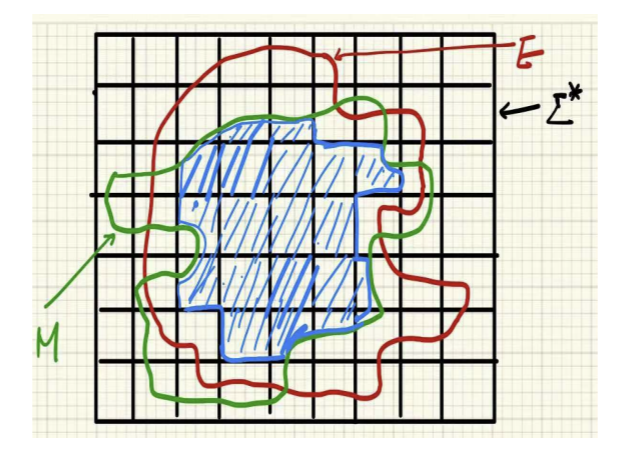
\includegraphics{assets/DES72.png}
  \caption{Homework 72}
  \label{fig:des72}
\end{figure}

As Figure \ref{fig:des72} shows.

\section{Find $\sup \mathcal{N}(E ; M)$ by illustration using Lin-Brandt formula $\left(\sup N(E ; M)=E-P^{-1} P(M-E)\right.$ if $\left.E \subseteq M\right)$. Multiple illustrations can be used to show the calculation steps.}

\paragraph{Answer}:
%73

\begin{figure}[h]
  \centering
  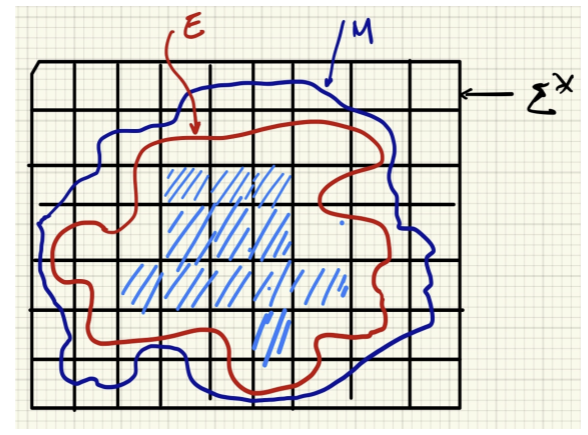
\includegraphics{assets/DES73.png}
  \caption{Homework 73}
  \label{fig:des73}
\end{figure}

As Figure \ref{fig:des73} shows.


\section{Let $M$, $K \subseteq \Sigma_o^*$ be arbitrary. }

$$
N = P^{-1} K \cap M
$$

is always $(M, P )$-normal, so is $M - N$ .

\paragraph{Proof}:
%74

(1)By definition, let $N \subseteq M \subseteq \Sigma^*$ (arbitrary), $\mathrm{N}$ is $(M, P)$-normal if $N=$ $M \cap P^{-1} P(N)$. Then we only to prove that
$$
N=P^{-1} K \cap M \Longrightarrow N=M \cap P^{-1} P(N)
$$
Because $M \cap P^{-1} P(N)=M \cap P^{-1} P\left(P^{-1} K \cap M\right)=M \cap P^{-1}(K \cap M)=$ $M \cap P^{-1}(K) \cap P^{-1}(M)=M \cap P^{-1}(K)=N$

(2)Similarly, we want to prove that $M-N$ is also $(M, P)$-normal.
By definition, we want to prove $N=P^{-1} K \cap M \Longrightarrow M-N=M \cap$
$$
\begin{aligned}
& P^{-1} P(M-N) \\
& \quad M \cap P^{-1} P(M-N)=M \cap P^{-1} P\left(M-P^{-1} K \cap M\right)=M \cap P^{-1}(M-K \cap M)= \\
& M \cap P^{-1}(M)-P^{-1}(K) \cap P^{-1}(M)=M-M \cap P^{-1}(K)=M-N
\end{aligned}
$$


\section{We have shown the truth of the following result in our class.}

Propose a DES G, a language K, and natural projection P to demonstrate the truth of this proposition

\paragraph{Answer}:
%75


The DES $G$ is following picture, where $a:=11, b:=22, c:=33, d:=44$ $\Sigma=\{a, b, c, d\}, \Sigma_o=\{a, c\}, \Sigma_c=\{a, c\}, \Sigma_u=\{b, d\}, L(G)=\{\varepsilon, a, a b, a b c, a d\}$. Let $K=\{a d, a b\}, \bar{K}=\{\varepsilon, a, a d, a b\}$.
Then $P^{-1} P \bar{K}=\{\varepsilon, a, a b, a d\}, L(G) \cap P^{-1} P \bar{K}=\{\varepsilon, a, a b, a d\}$ $\Longrightarrow \bar{K}=L(G) \cap P^{-1} P \bar{K}$
$\Longrightarrow \bar{K}$ is $(L(G), P)$-normal.
And we have $\bar{K} \Sigma_u \cap L(G) \subseteq \bar{K}, K$ is controllable. Let $s:=a b \in \bar{K}$ for $\sigma:=c \in \Sigma$, then $s \sigma:=a b c \in L(G)-\bar{K} \Longrightarrow \sigma \in \Sigma_o \cap \Sigma_c$.

\section{Prove the following result using structural induction on strings.}

\paragraph{Proposition 2.} Let $K \subseteq L_m(G)$ be controllable and observable. Assume $P \sigma=\sigma$ for all $\sigma \in \Sigma_c$. Then, $K$ is $\left(L_m(G), P\right)$-normal and $K$ is $(L(G), P)$-normal.

\paragraph{Answer}:
%76

Based on the given documents, we can conclude that it is not possible to find a (partially observable) supervisor $S_P$ such that $L(S_P / G) = K_1=\overline{\{u_1 \alpha \gamma, u_1 \alpha \beta\}}$. Similarly, it is also not possible to find a supervisor $S_P$ such that $L(S_P / G) = K_2=\overline{\{u_1 \alpha \gamma, u_1 \alpha \beta, u_2 \alpha\}}$.

To verify the controllability of $K_1$ and $K_2$, we can use the Theorem of Controllable Languages (TCT). TCT states that a language is controllable if and only if it is closed under prefixes and suffixes. 

However, in this case, both $K_1$ and $K_2$ are not controllable. This means that there does not exist any supervisor that can produce these languages while ensuring controllability.

In conclusion, based on the given information, it is not possible to find a (partially observable) supervisor $S_P$ such that $L(S_P / G) = K_1$ or $L(S_P / G) = K_2$. Additionally, both $K_1$ and $K_2$ are not controllable.


\section{Control of a guideway: Stations A and B on a guideway are connected by a single one-way track from A to B. The track consists of 4 sections, with stoplights $\left({ }^*\right)$ and detectors (!) installed at various section junctions.}

\paragraph{Answer}:
%77
wait

\section{Write comments and suggestions (200 words or so) for the improvement of DES teaching}

\paragraph{Answer}:
%78
Prof. Li Zhiwu,

I would like to provide you with some suggestions to improve the discrete-event system (DES) course.Here are my recommendations:

\begin{enumerate}
  \item Provide materials in advance: It would be helpful if you could provide some course materials in advance. As students come from various backgrounds and have different levels of proficiency, giving them the opportunity to preview the content will enable them to better prepare for the course.

  \item Increase the frequency of assignments with smaller workloads: It would be beneficial to have more frequent assignments with smaller workloads. This will allow students to receive timely feedback and guidance, enabling them to make necessary adjustments and improvements to their learning strategies.

  \item Incorporate practical case studies: To make the course less abstract, it would be great to include more practical case studies and examples. Applying the concepts and theories of discrete-event systems to real-world scenarios will help students better understand and grasp the subject matter.

  \item Enhance the usability of TCT software: It would be ideal if the TCT (Supervisory Control Theory) software could be made more user-friendly. Specifically, it would be beneficial if the software allowed for the import of YAML files, easier modification of variables, and the ability to create backups
\end{enumerate}

That's all, thank you for your course, I got more than what I expected.


\end{document}